\documentclass[titlepage,11pt]{article}
\usepackage[utf8]{inputenc}  % Load inputenc first
\usepackage{comment}
\usepackage{enumitem}
\usepackage{listings}
\usepackage{amsmath}
\usepackage{graphicx}
\usepackage[font=small,labelfont=bf]{caption}
\usepackage[bahasa]{babel}
\usepackage{float}
\usepackage{verbatim}
\usepackage{graphicx,tabularx,multirow}
\usepackage{xcolor}
\usepackage[onehalfspacing]{setspace}
\usepackage[
	allcolors=visigrey,
	colorlinks=true,
]{hyperref}
\usepackage[a4paper,left=2cm,right=2cm]{geometry}
\usepackage{csquotes}
% Pengaturan kutipan artikel
\usepackage[style=ieee, backend=biber]{biblatex}
% Code listing style pak akok
\definecolor{codegreen}{rgb}{0,0.6,0}
\definecolor{codegray}{rgb}{0.5,0.5,0.5}
\definecolor{codepurple}{rgb}{0.58,0,0.82}
\definecolor{backcolour}{rgb}{0.95,0.95,0.92}

% Ubah sesuai modul
 \addbibresource{P1/pustaka/pustaka.bib}
% \addbibresource{P2/pustaka/pustaka.bib}
% \addbibresource{P3/pustaka/pustaka.bib}
% \addbibresource{P4/pustaka/pustaka.bib}
% \addbibresource{P5/pustaka/pustaka.bib}

\lstdefinestyle{mystyle}{
	backgroundcolor=\color{backcolour}, commentstyle=\color{codegreen},
	keywordstyle=\color{magenta},
	numberstyle=\small\color{codegray},
	stringstyle=\color{codepurple},
	basicstyle=\ttfamily\footnotesize,
	breakatwhitespace=false,         
	breaklines=true,                 
	captionpos=t,                    
	keepspaces=true,                 
	numbers=left,                    
	numbersep=5pt,                  
	showspaces=false,                
	showstringspaces=false,
	showtabs=false,           
	frame = single,
	tabsize=2
}
\lstset{style=mystyle}

\definecolor{visigrey}{rgb}{.1,.15,.15}
\geometry{top=1cm,bottom=.5cm}
\savegeometry{titlepage}
\geometry{top=2cm,bottom=2cm}
\savegeometry{main}

\def\bspace{\(\qquad\qquad\qquad\)}
\usepackage[T1]{fontenc}
\usepackage[utf8]{inputenc}
\usepackage{tgheros}
\renewcommand*\familydefault{\sfdefault}

\setcounter{tocdepth}{6}

\def\autor{Laboratorium }
\def\lab{Multimedia dan Internet of Things}
\def\departemen{Departemen Teknik Komputer}
\def\institut{Institut Teknologi Sepuluh Nopember}
\def\praktikum{Praktikum \\ Pengolahan Sinyal Digital}
% Ubah Judul sesuai dengan modul
 \def\judul{Function Generator dan Osiloskop}
% \def\judul{(ADC) Analog to Digital Converter}
% \def\judul{(DAC) Digital to Analog Converter}
% \def\judul{Digital Filter}
% \def\judul{Fourier Transform}
\def\tahun{2024}

\begin{document}
% Ubah Bahasa sesuai dengan keinginan
\selectlanguage{bahasa}
\input{Cover/Header.tex}
% Pilih Modul yang akan di build
 \section{Pendahuluan}
\subsection{Latar Belakang}

Pada modul pertama, praktikan mempelajari penggunaan osiloskop dan function generator.
Proses pengolahan sinyal digital, peralatan pengukuran dan pengujian sangatlah penting untuk memastikan bahwa sinyal yang diolah telah sesuai dengan spesifikasi yang diinginkan. Dalam konteks ini, osiloskop dan function generator merupakan peralatan yang sangat fundamental.
\\\\
Osiloskop merupakan alat ukur elektronik yang digunakan untuk melakukan visualisasi sinyal listrik dalam bentuk gelombang. Dengan osiloskop, kita dapat mengamati perubahan tegangan seiring waktu, yang sangat berguna untuk menganalisis karakteristik sinyal dalam rangkaian elektronik.
Osiloskop memungkinkan pengguna untuk: mengukur frekuensi dan periode sinyal, mengamati bentuk gelombang dan mendeteksi distorsi atau noise, mengukur tegangan puncak ke puncak (Vpp) dan tegangan rata-rata, dan menganalisis hubungan fasa antara dua sinyal.
\\\\
Function generator adalah alat yang digunakan untuk menghasilkan berbagai bentuk gelombang listrik, seperti gelombang sinus, persegi, segitiga, dan gigi gergaji. 
Function generator sangat berguna dalam pengujian dan pengembangan rangkaian elektronik karena memungkinkan pengguna untuk: menghasilkan sinyal dengan frekuensi dan amplitudo yang dapat diatur, menguji respons rangkaian terhadap berbagai bentuk gelombang, dan mensimulasikan kondisi operasi yang berbeda dalam rangkaian.

\subsection{Maksud dan Tujuan}
Mengetahui dan memahami dasar penggunaan osiloskop dan function generator.

\subsection{Hasil yang diharapkan}
Dapat memahami dasar penggunaan osiloskop dan function generator.

%===========================================================%
\section{Tugas Pendahuluan}
\begin{enumerate}
\item Buatlah
\end{enumerate}

%===========================================================%
\section{Alat dan Bahan}
\begin{itemize}[label=$\bullet$, itemsep=-1pt, leftmargin=*]
	\item Function generator
	\item Osiloskop
	\item Kabel probe
\end{itemize}

%===========================================================%
\section{Jangka Waktu Pelaksanaan}
Pemahaman dan konfigurasi 30 menit.

%===========================================================%

\section{Proses dan Tahapan Konfigurasi}
%======================PERCOBAAN 1==========================%
\subsection{Percobaan 1}
\begin{center}

	\textbf{Konfigurasi Osiloskop}
	\begin{enumerate}
		\item Hubungkan kabel power ke osiloskop, lalu tekan tombol power untuk menyalakan Osiloskop. 
			\begin{figure}[H]
				\centering
				\includegraphics[width=0.8\linewidth]{P1/img/per 1/step 1.png}
				\caption{Step 1}
				\label{fig:Step 1(Group 7)}
			\end{figure}

		\item Hubungkan kabel probe pada channel 1.
			\begin{figure}[H]
				\centering
				\includegraphics[width=0.8\linewidth]{P1/img/per 1/step 2.png}
				\caption{Step 2}
				\label{fig:Step 2(Group 14)}
			\end{figure}

		\item Hubungkan probe pengait pada pengkalibrasi osiloskop.
			\begin{figure}[H]
				\centering
				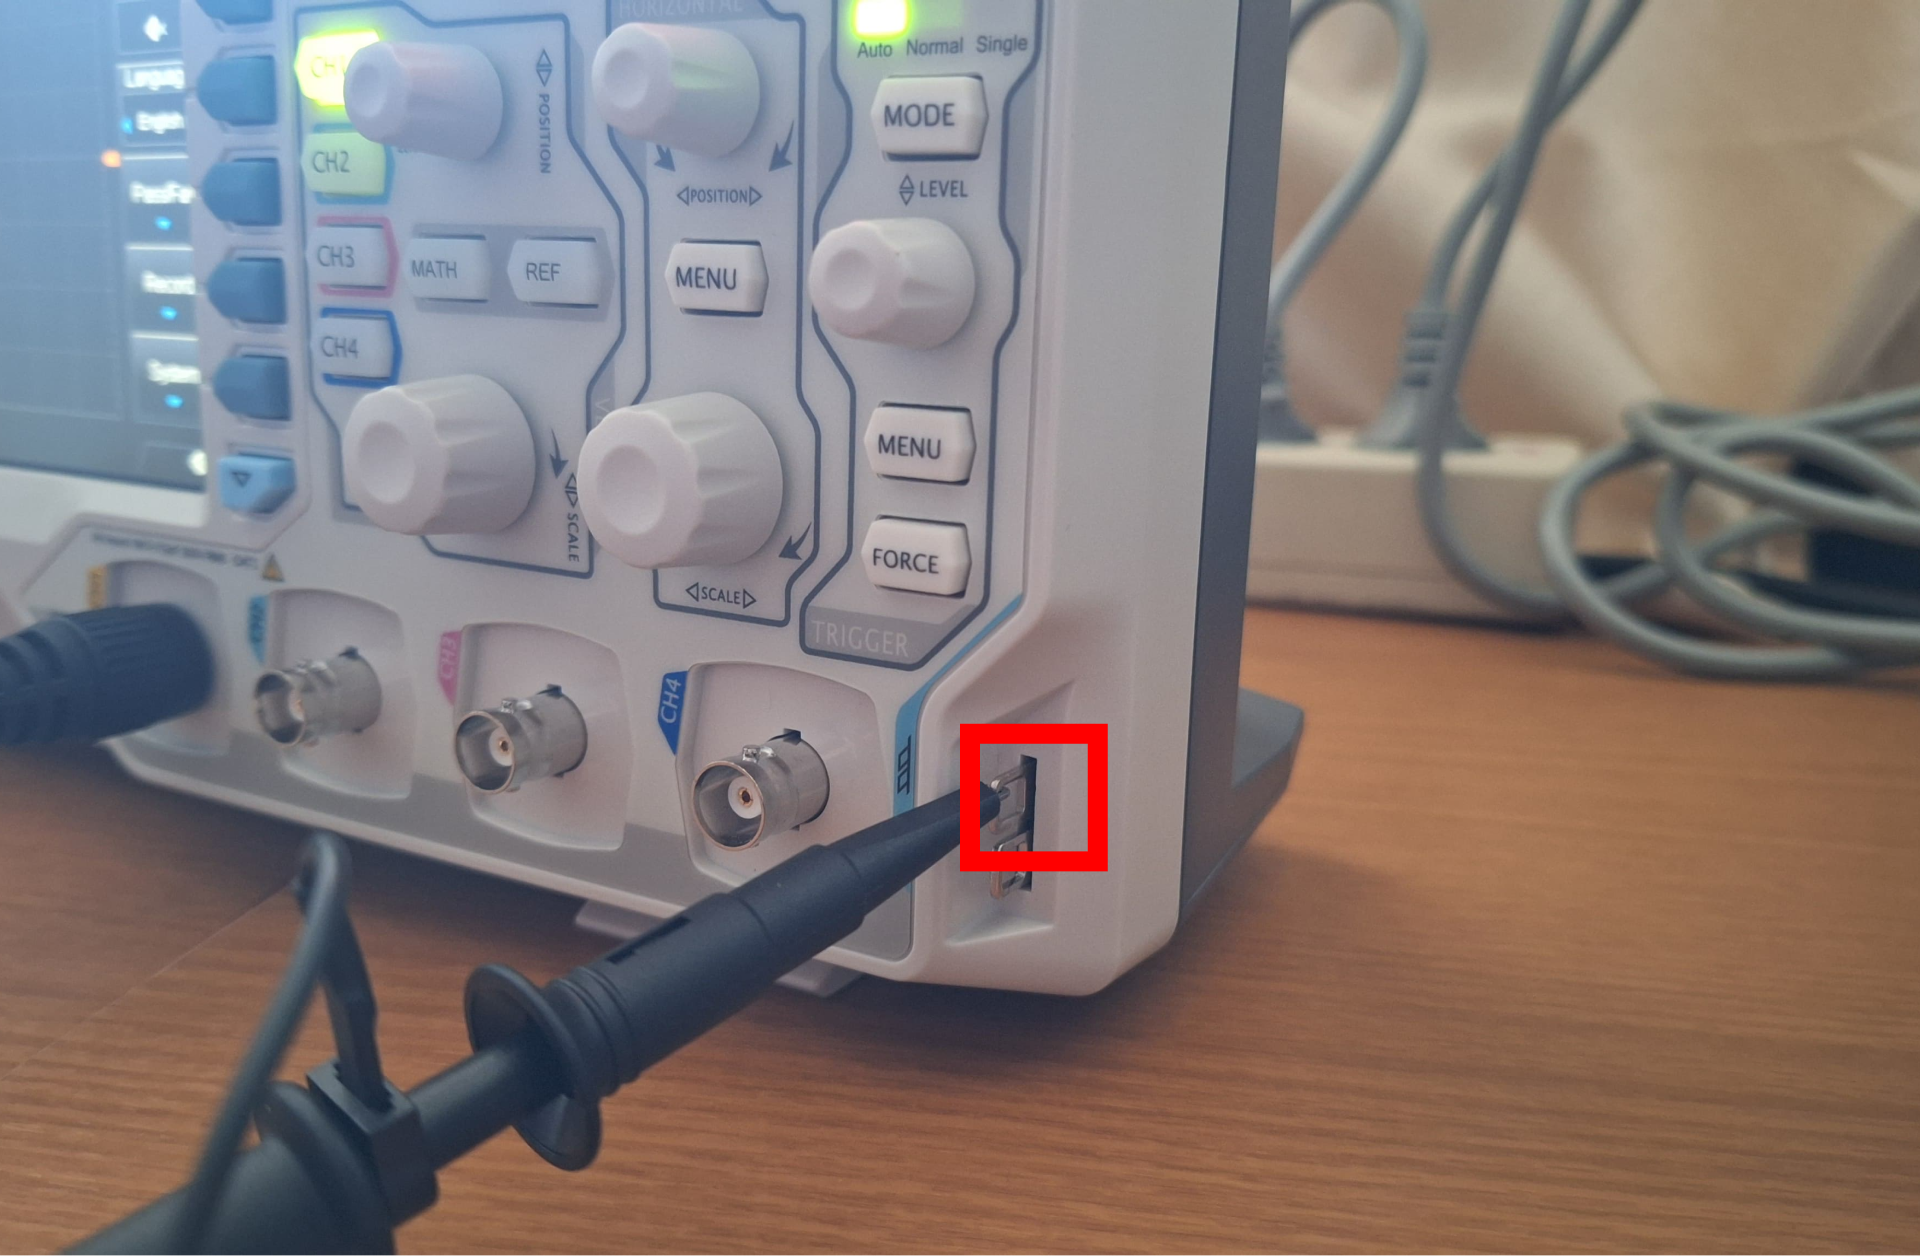
\includegraphics[width=0.8\linewidth]{P1/img/per 1/step 3.png}
				\caption{Step 3}
				\label{fig:Step 3(Group 15)}
			\end{figure}

	\item Tekan tombol AUTO pada osiloskop, lalu sinyal akan muncul setelah kalibrasi.
	\begin{figure}[H]
		\centering
		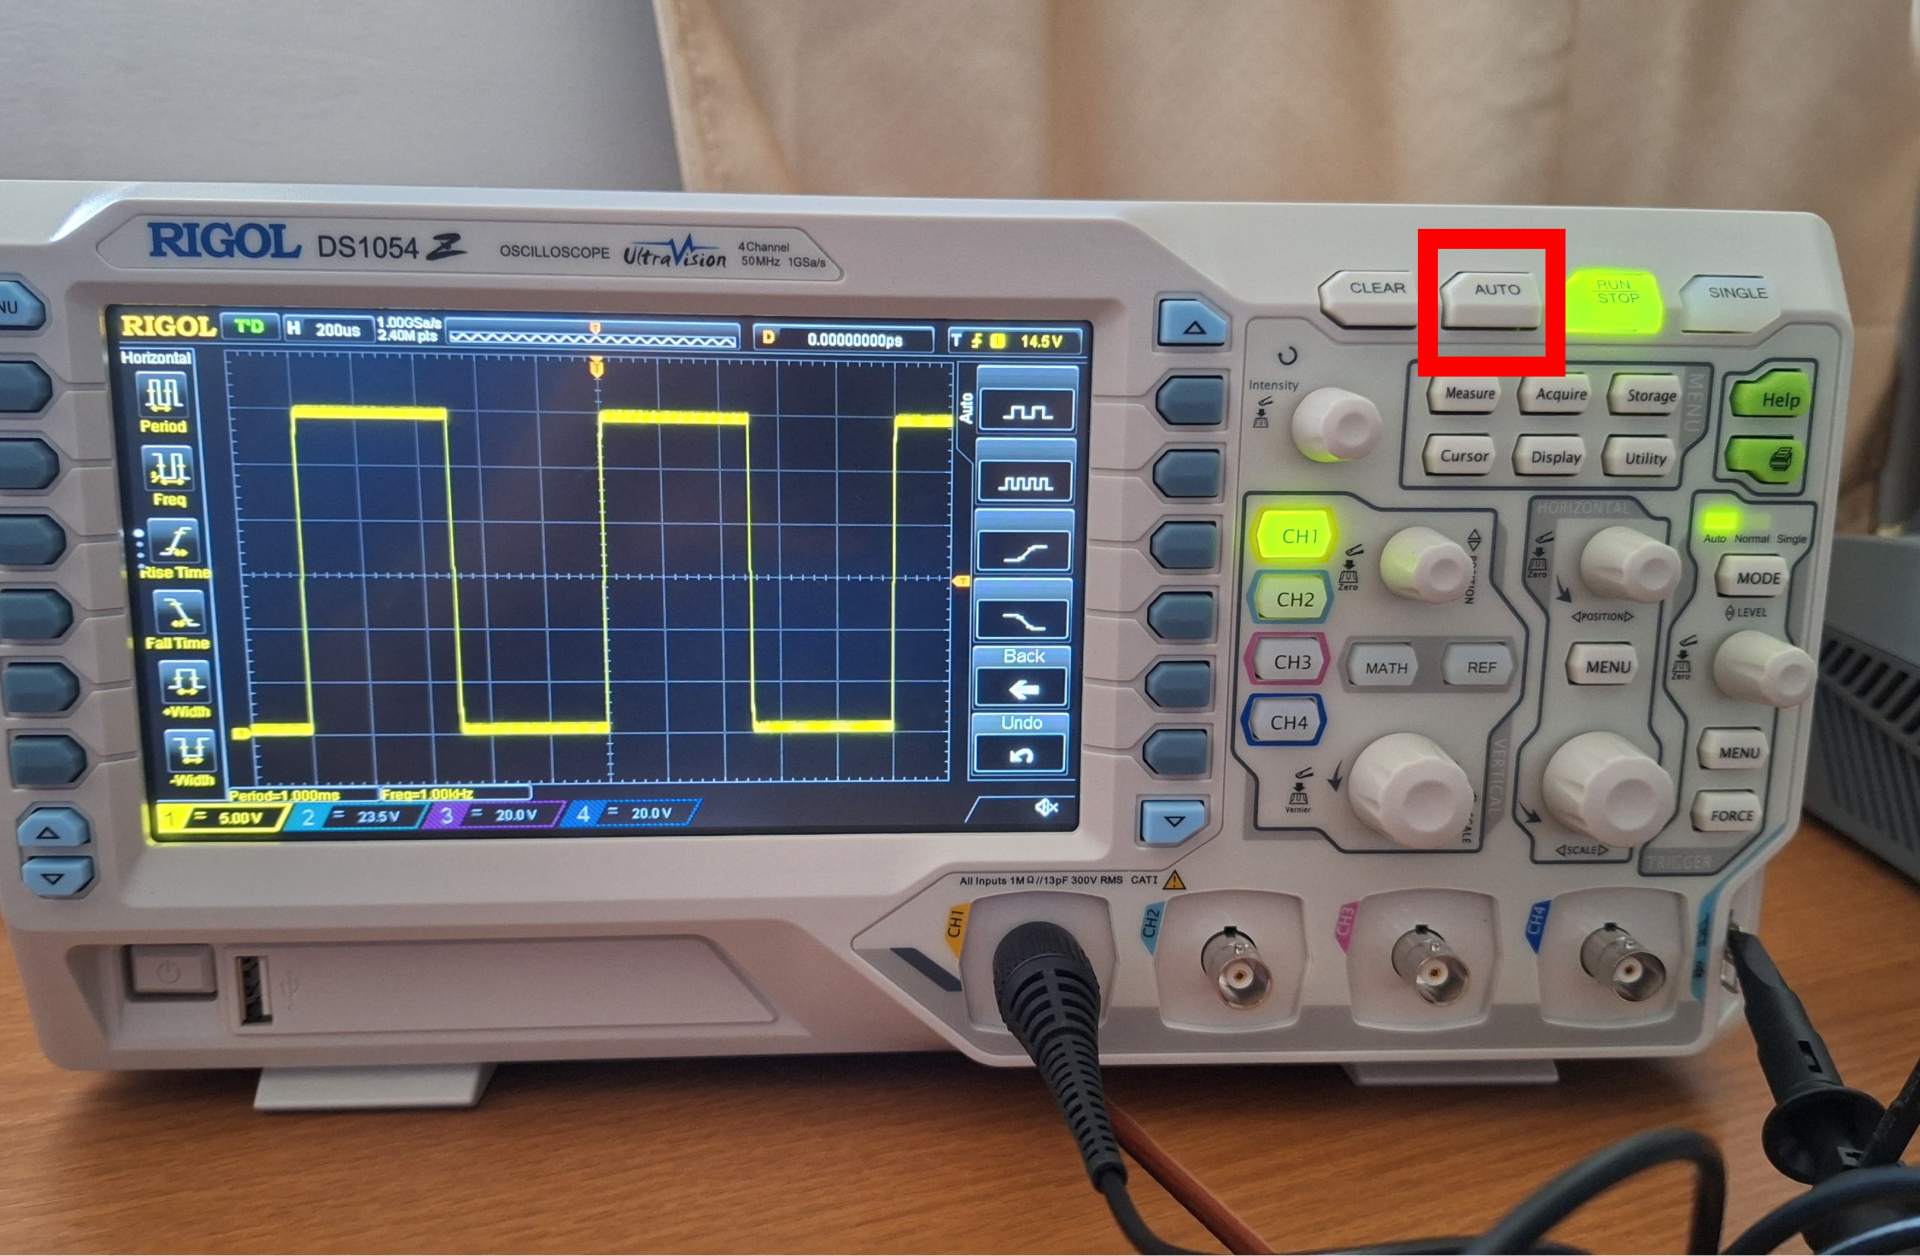
\includegraphics[width=0.8\linewidth]{P1/img/per 1/step 4.png}
		\caption{Step 4}
		\label{fig:Ping Step 4(Group 4)}
	\end{figure}
	\end{enumerate}
\end{center}

%======================PERCOBAAN 2==========================%
\subsection{Percobaan 2}
\begin{center}

	\textbf{Konfigurasi Osiloskop dan Function generator}
	\begin{enumerate}
		\item Hubungkan kabel power ke function generator, lalu tekan tombol power untuk menyalakan Function generator.
		      \begin{figure}[H]
			      \centering
			      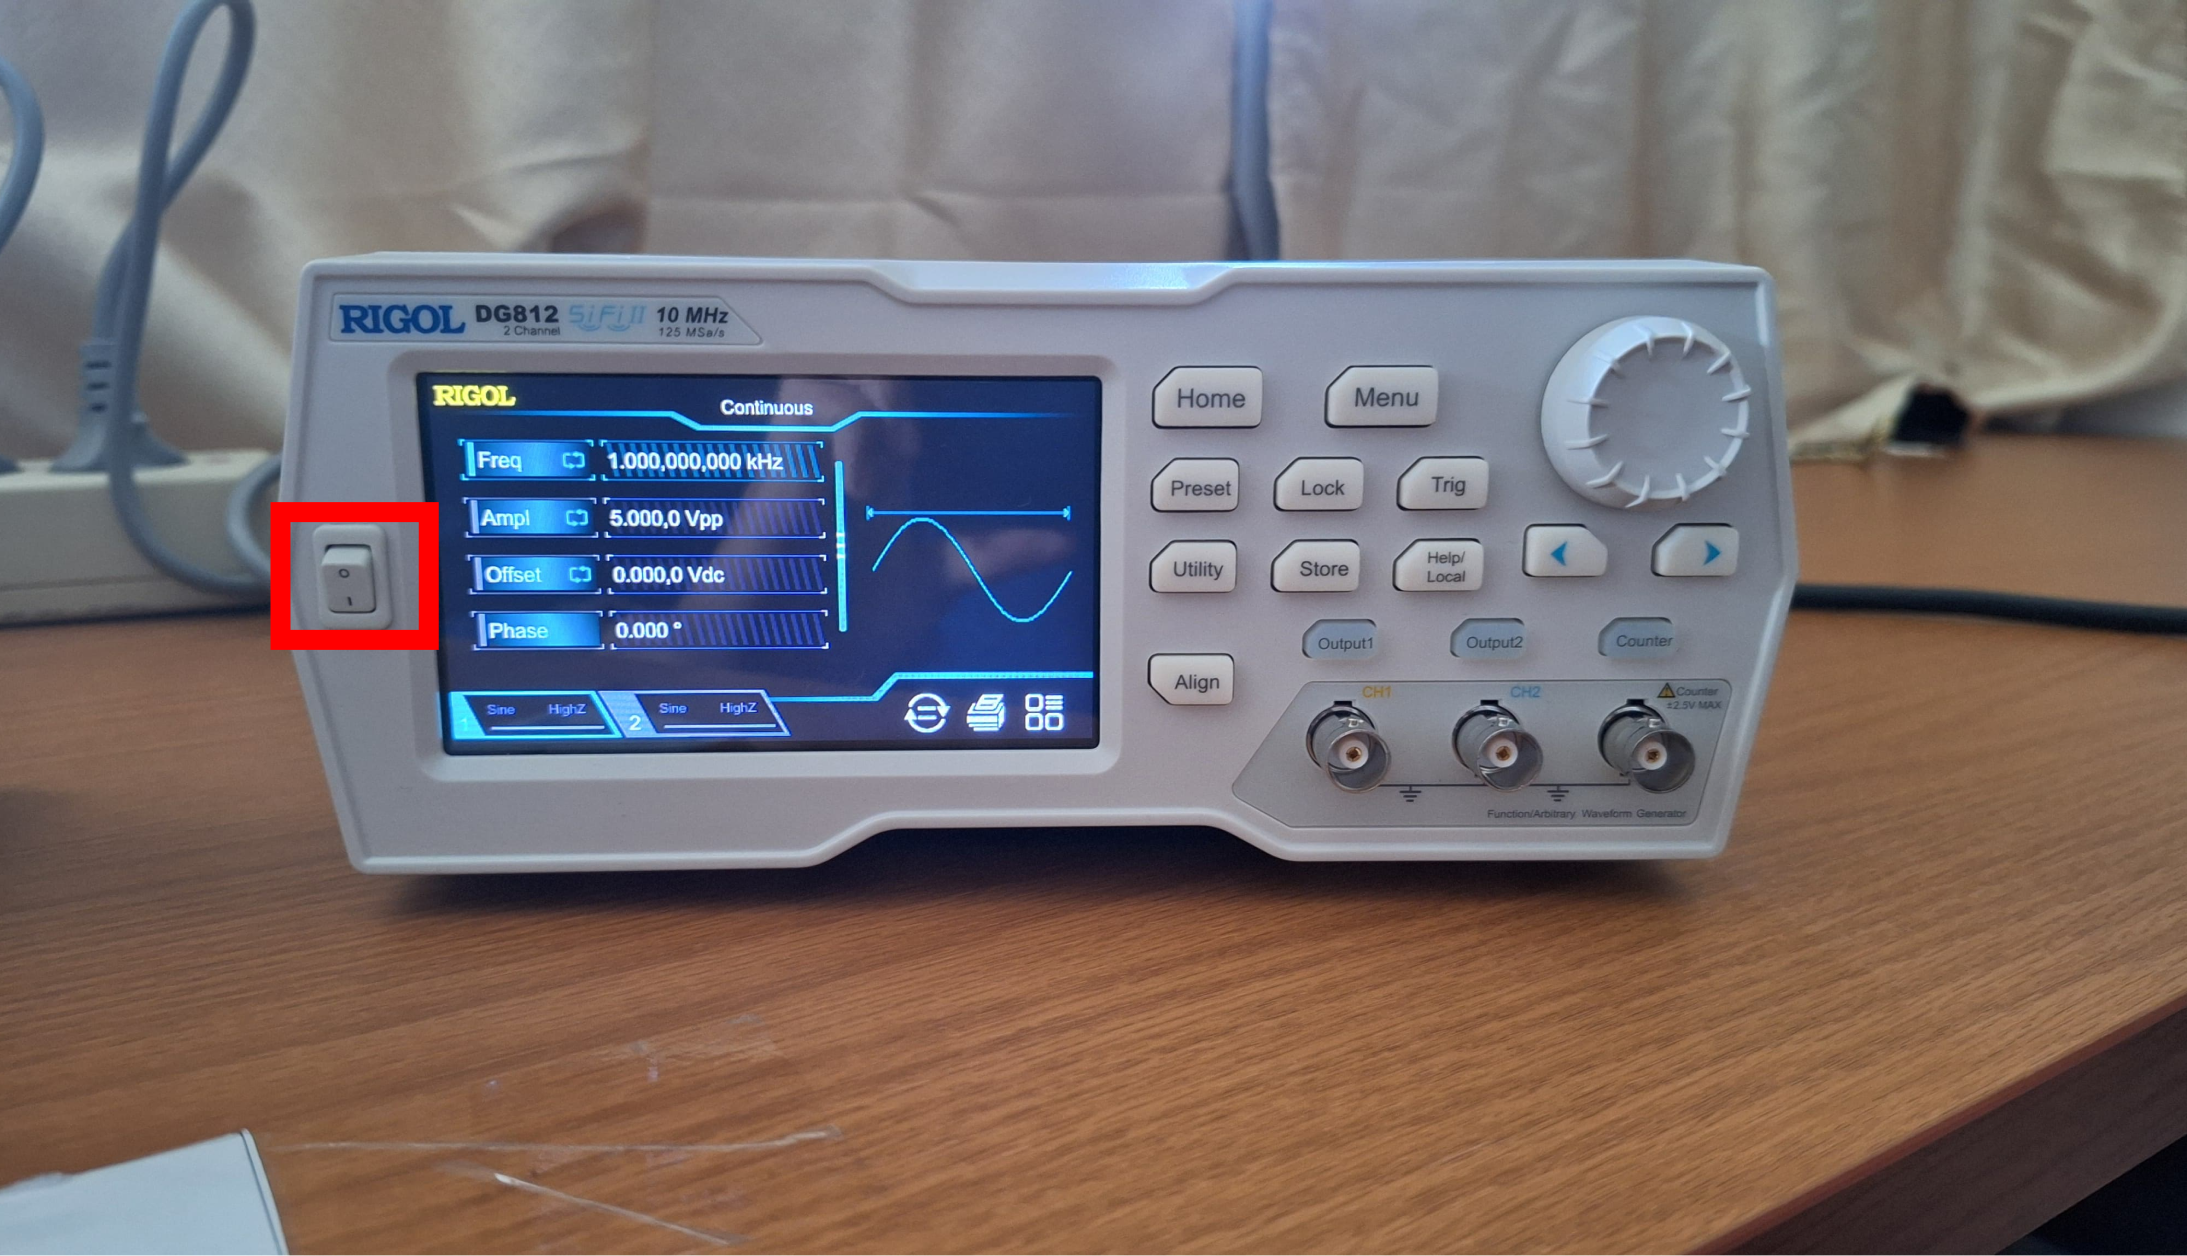
\includegraphics[width=0.8\linewidth]{P1/img/per 2/step 1.png}
			      \caption{Step 1}
			      \label{fig:Step 1(Group 7)}
		      \end{figure}

		\item Hubungkan kabel probe pada channel 1 osiloskop.
		      \begin{figure}[H]
			      \centering
			      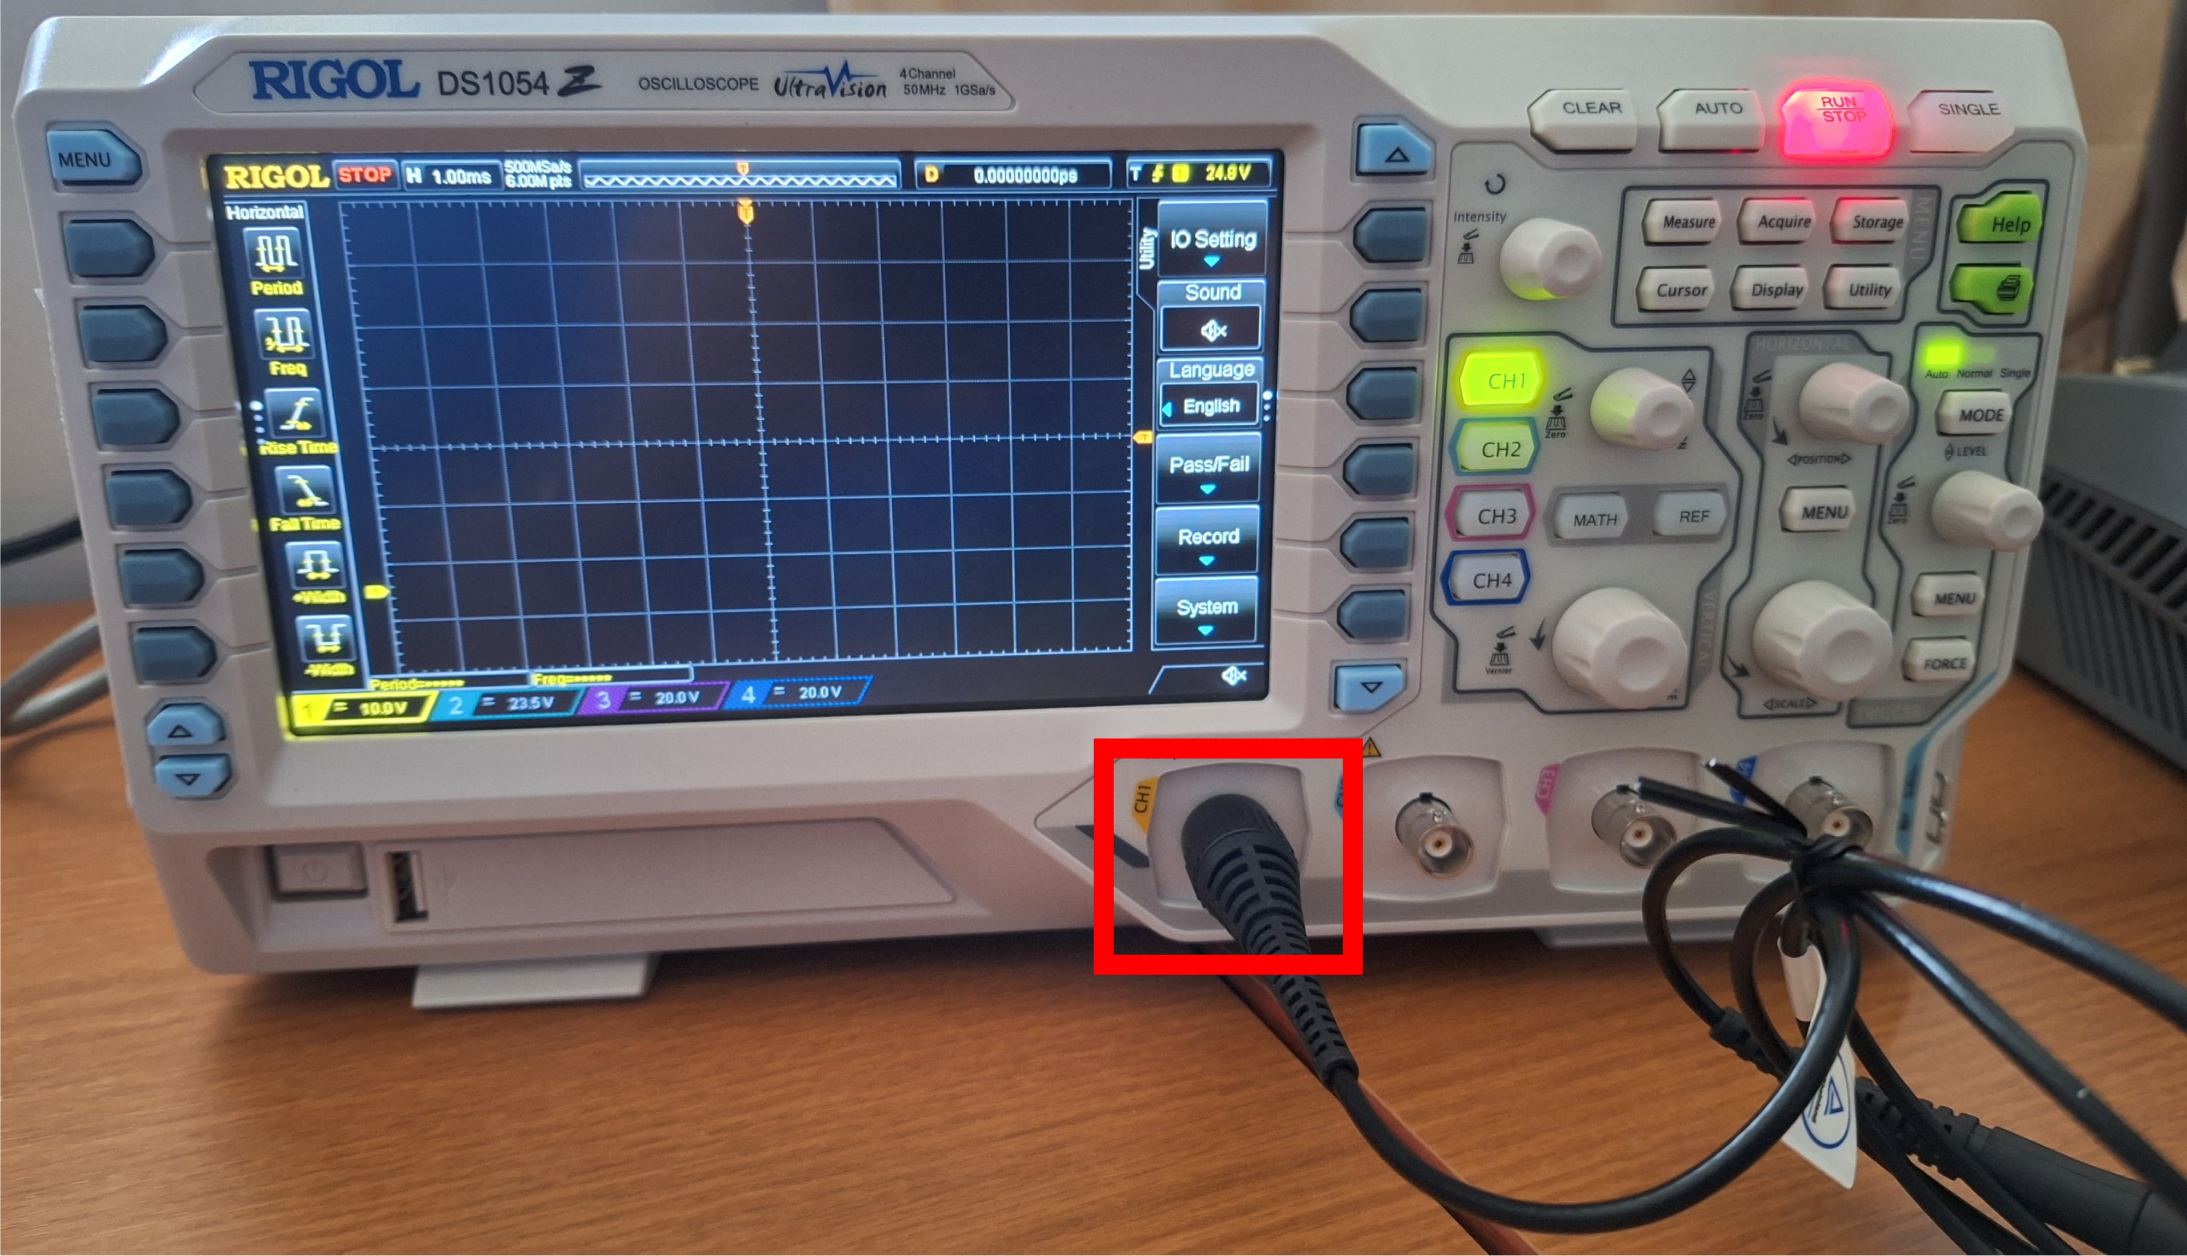
\includegraphics[width=0.8\linewidth]{P1/img/per 2/step 2.png}
			      \caption{Step 2}
			      \label{fig:Step 2(Group 8)}
		      \end{figure}

		\item Hubungkan kabel probe pada output 1 function generator.
		      \begin{figure}[H]
			      \centering
			      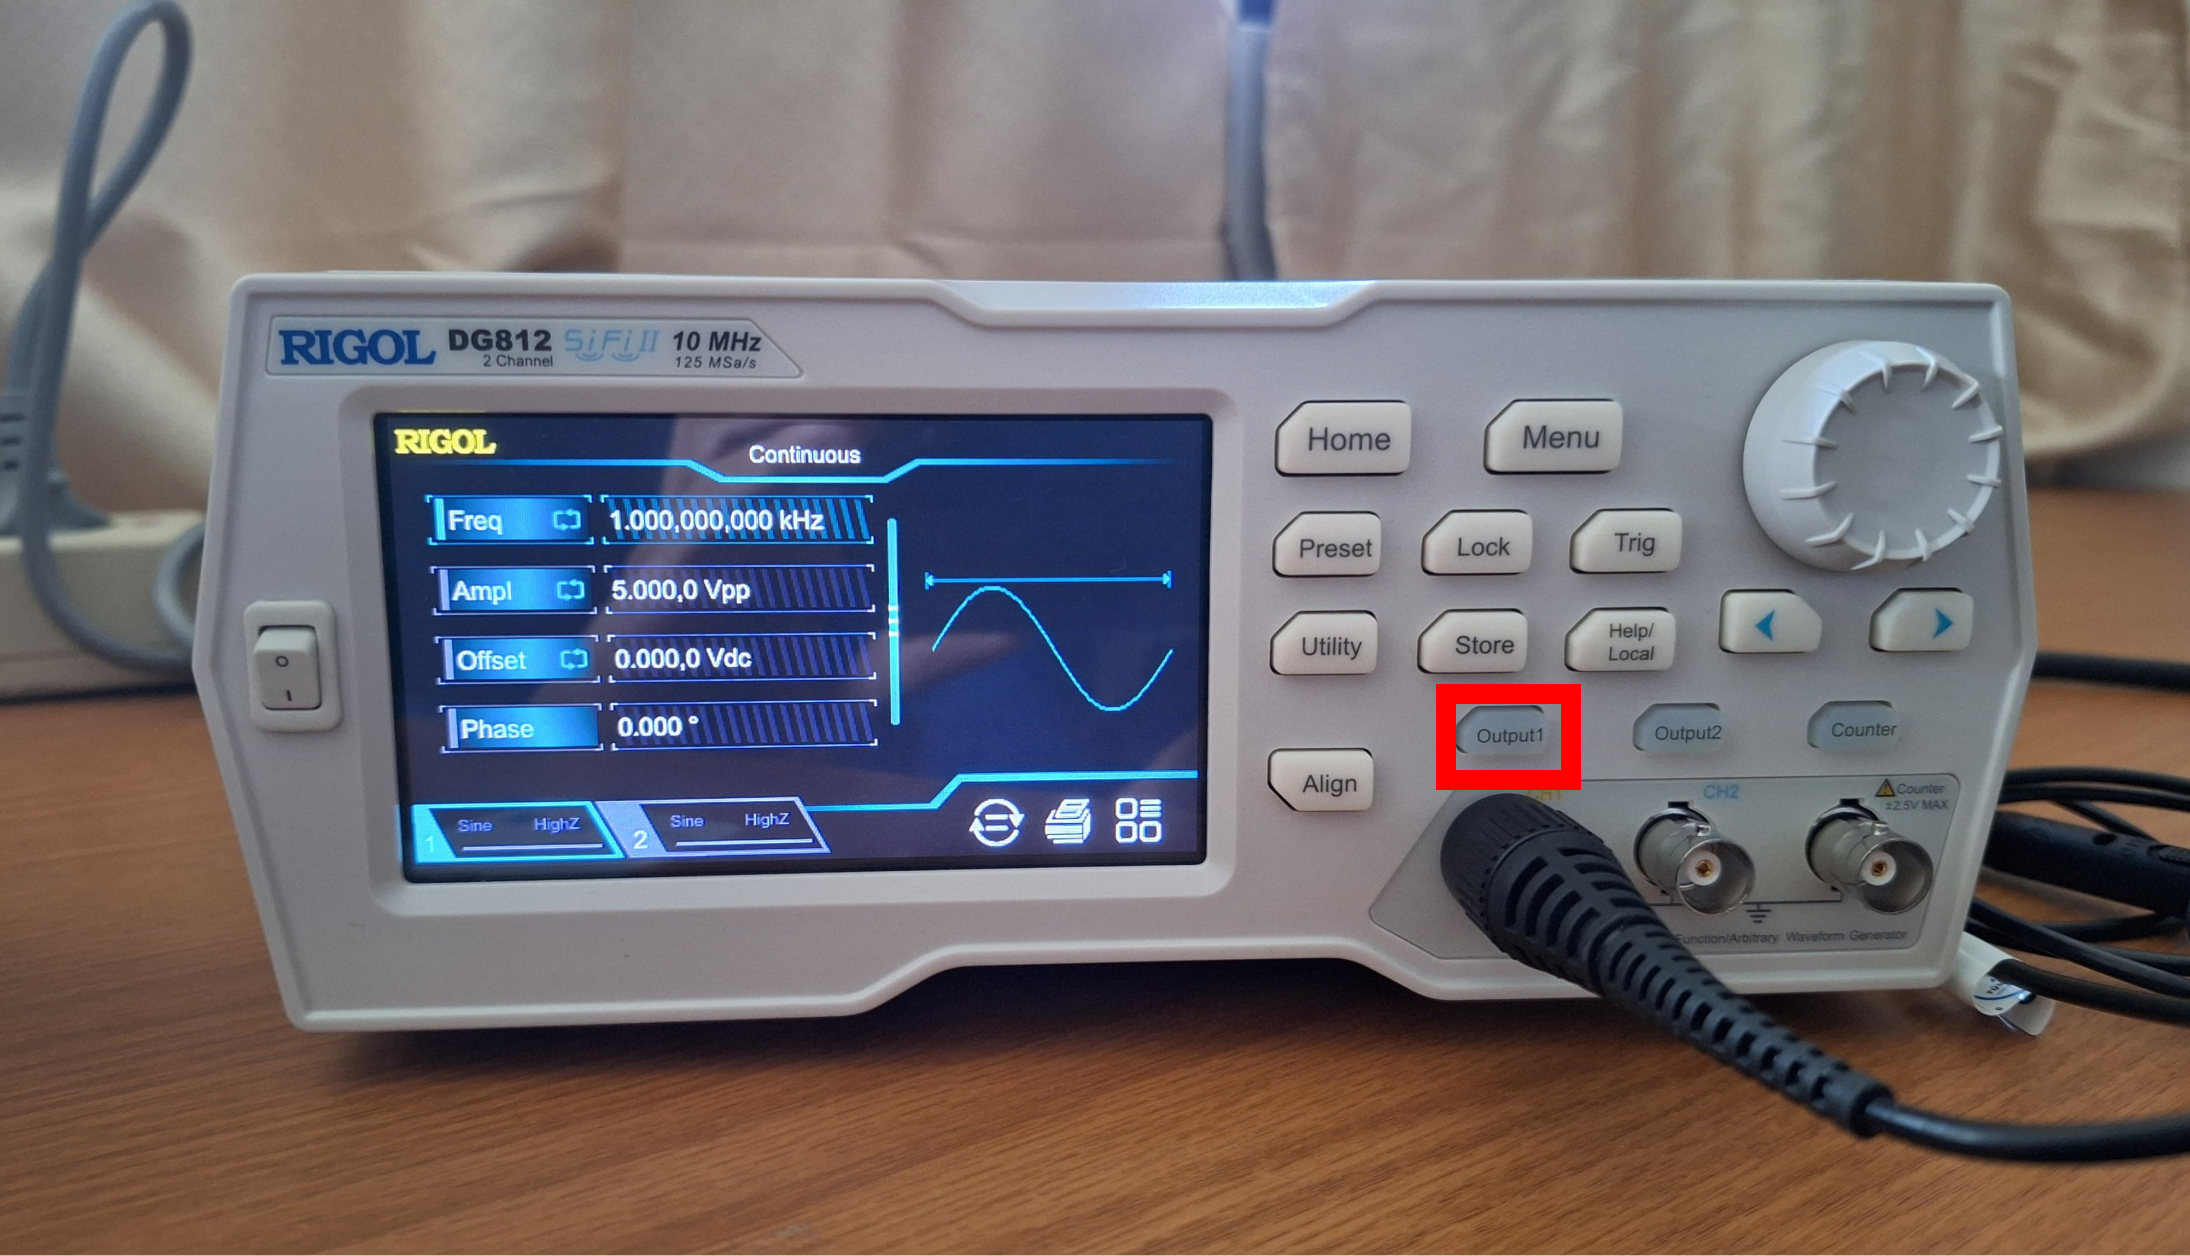
\includegraphics[width=0.8\linewidth]{P1/img/per 2/step 3.png}
			      \caption{Step 3}
			      \label{fig:Step 3(Group 9)}
		      \end{figure}

		\item Hubungkan probe pengait dari osiloskop dan function generator.
		      \begin{figure}[H]
			      \centering
			      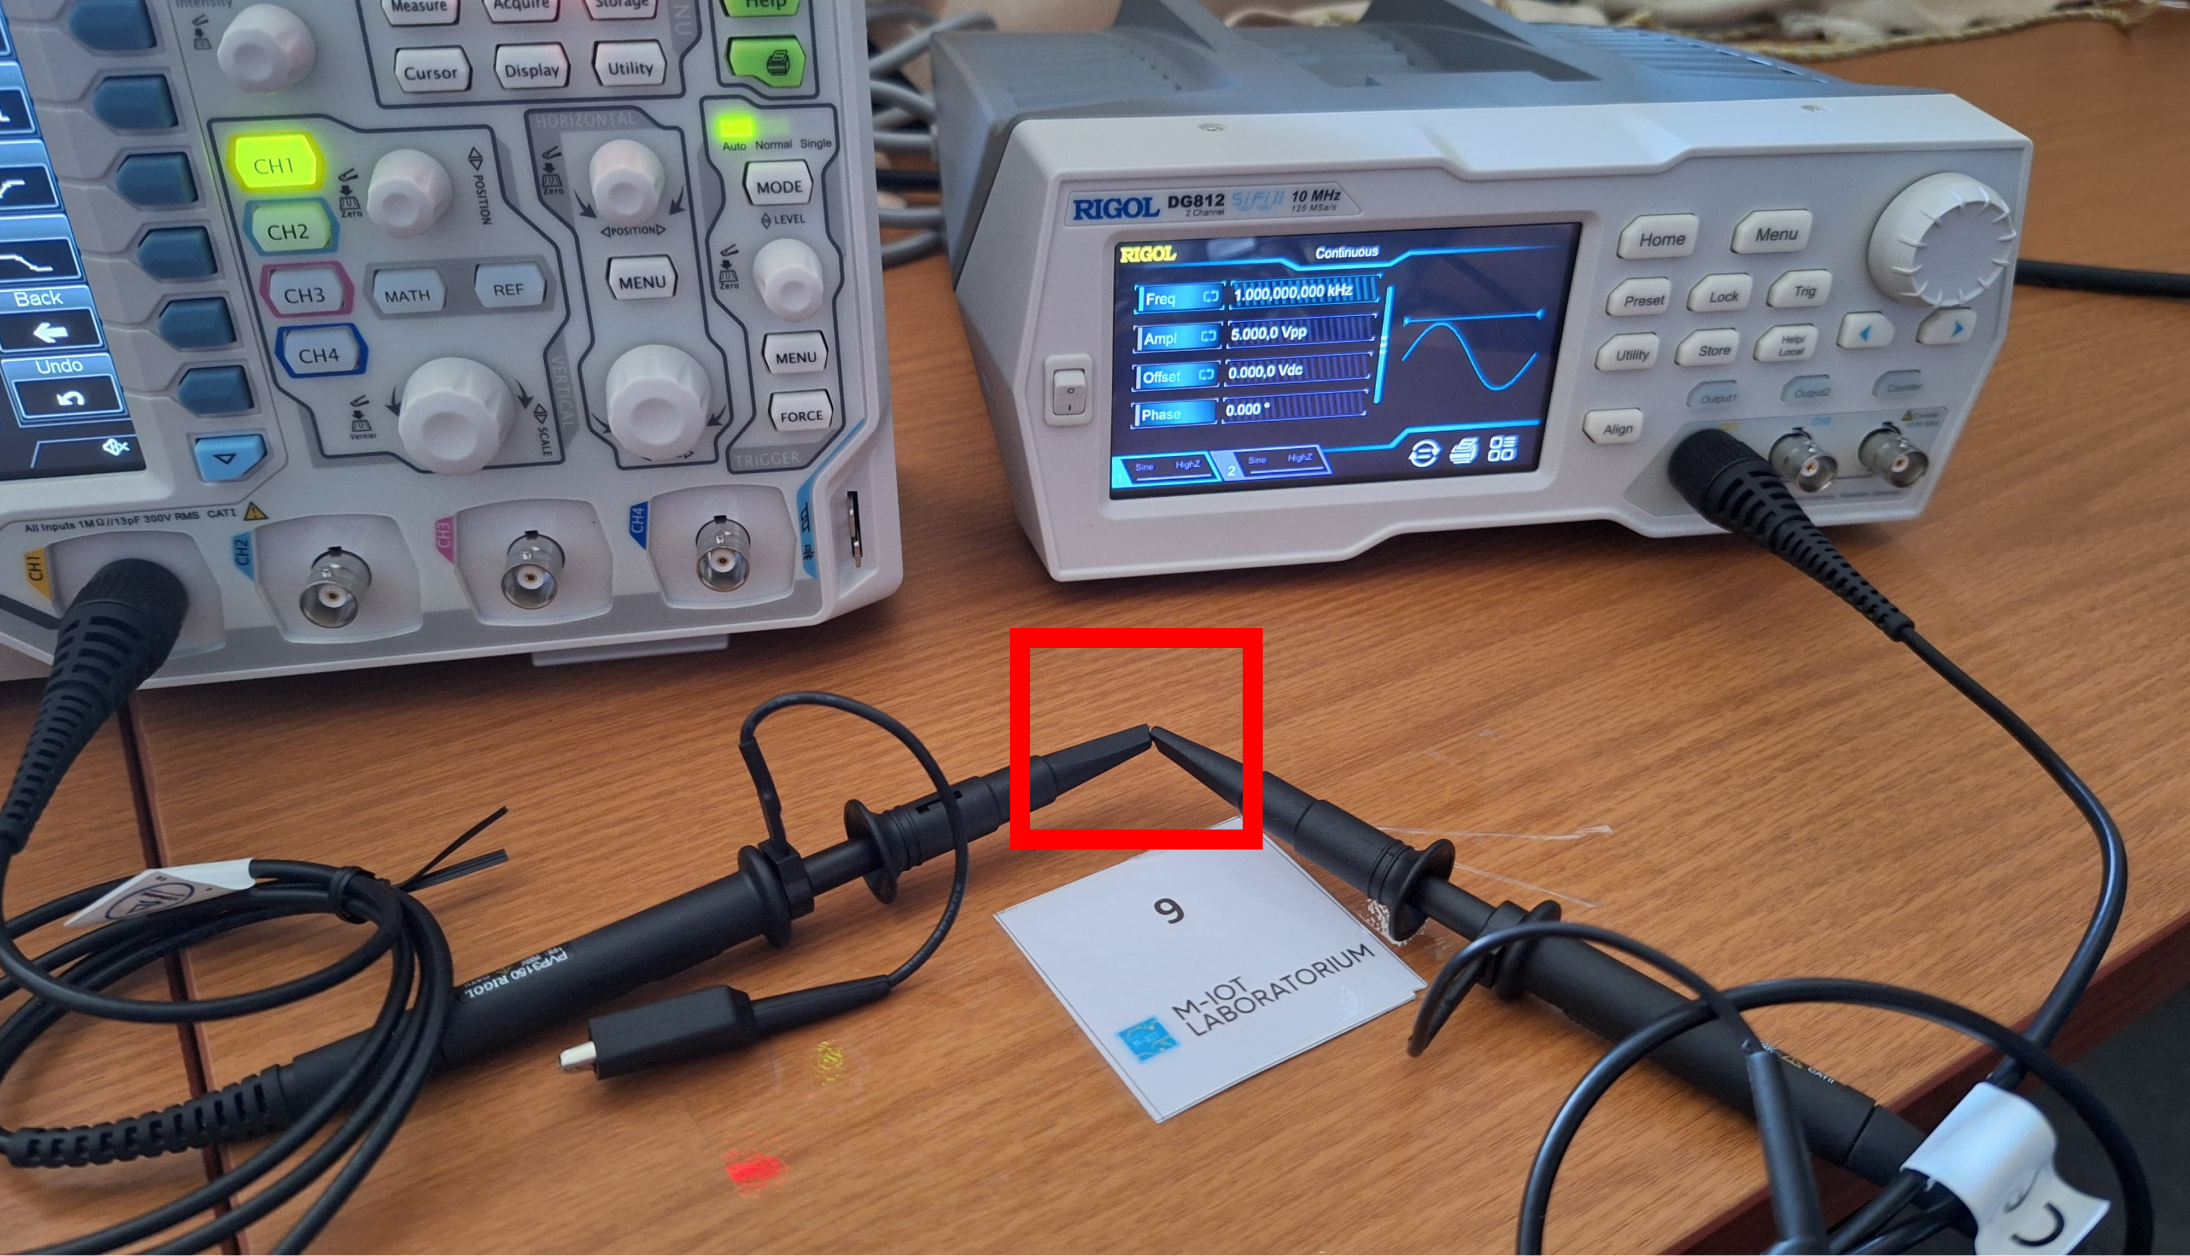
\includegraphics[width=0.8\linewidth]{P1/img/per 2/step 4.png}
			      \caption{Step 4}
			      \label{fig:Step 4(Group 10)}
		      \end{figure}

		\item Tekan tombol output 1 function generator.
		      \begin{figure}[H]
			      \centering
			      \includegraphics[width=0.8\linewidth]{P1/img/per 2/step 5.png}
			      \caption{Step 5}
			      \label{fig:Step 5(Group 11)}
		      \end{figure}

		\item Tekan tombol AUTO pada osiloskop.
		      \begin{figure}[H]
			      \centering
			      \includegraphics[width=0.8\linewidth]{P1/img/per 2/step 6.png}
			      \caption{Step 6}
			      \label{fig:Step 6(Group 12)}
		      \end{figure}

		\item Matikan output terlebih dahulu setiap ingin mengatur function generator.
		      \begin{figure}[H]
			      \centering
			      \includegraphics[width=0.8\linewidth]{P1/img/per 2/step 7.png}
			      \caption{Step 7}
			      \label{fig:Step 7(Group 16)}
		      \end{figure}

		\item Tekan tombol Home kemudian ganti ke bentuk sinyal kotak dengan menggunakan 
		\\analog putarnya dan panah kanan/kiri. Jika sudah, tekan analognya untuk klik.
		      \begin{figure}[H]
			      \centering
			      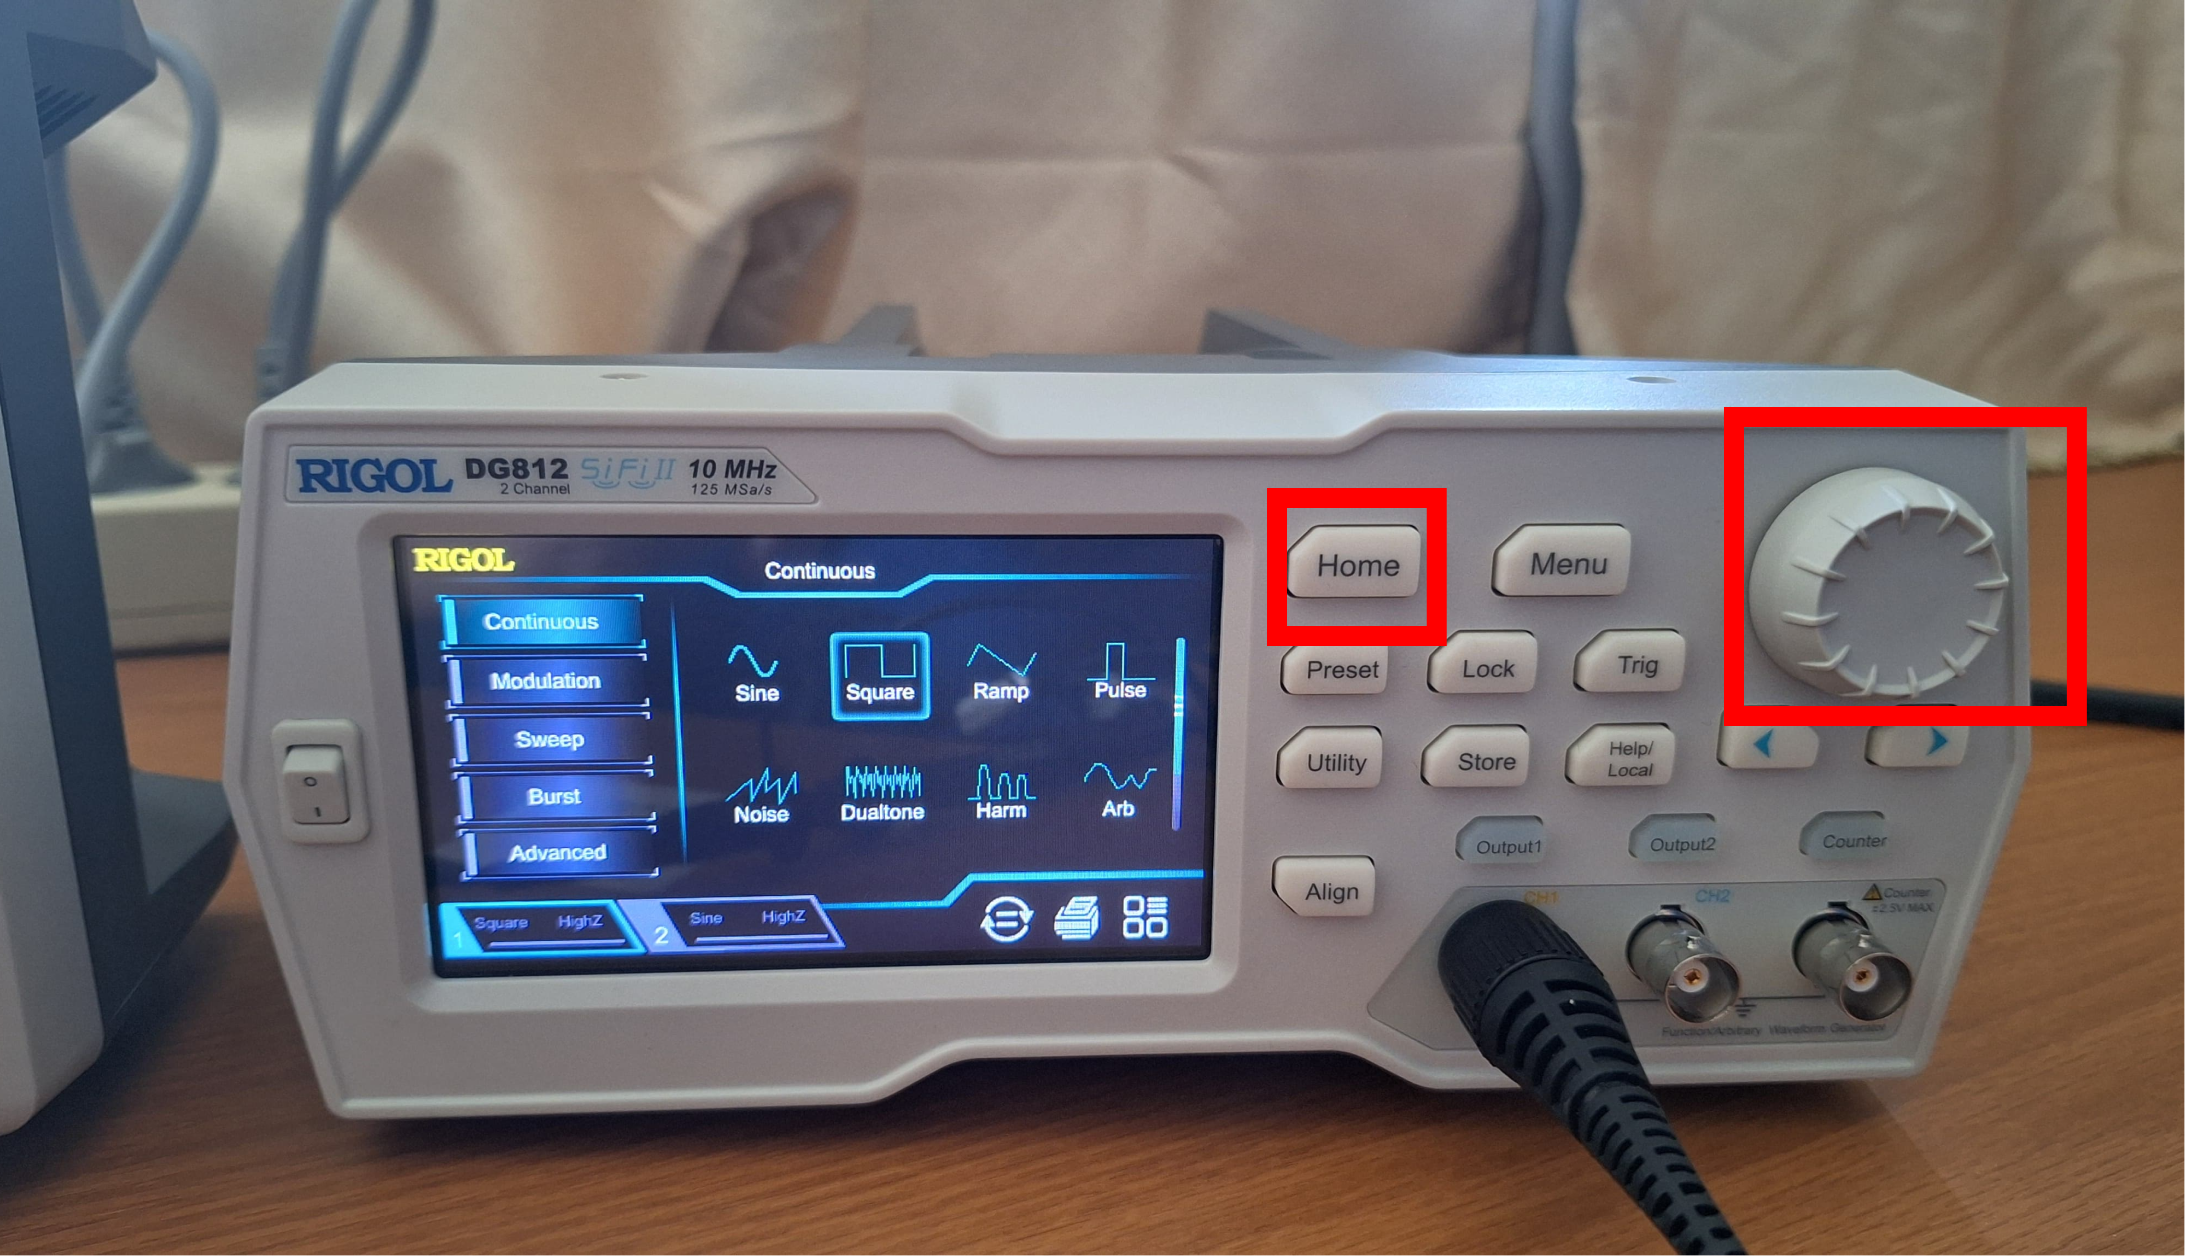
\includegraphics[width=0.7\linewidth]{P1/img/per 2/step 8.png}
			      \caption{Step 8}
			      \label{fig:Step 8(Group 13)}
		      \end{figure}

		\item Tekan Menu untuk kembali, lalu tekan output 1 untuk mengirimkan sinyal ke osiloskop.
		      \begin{figure}[H]
			      \centering
			      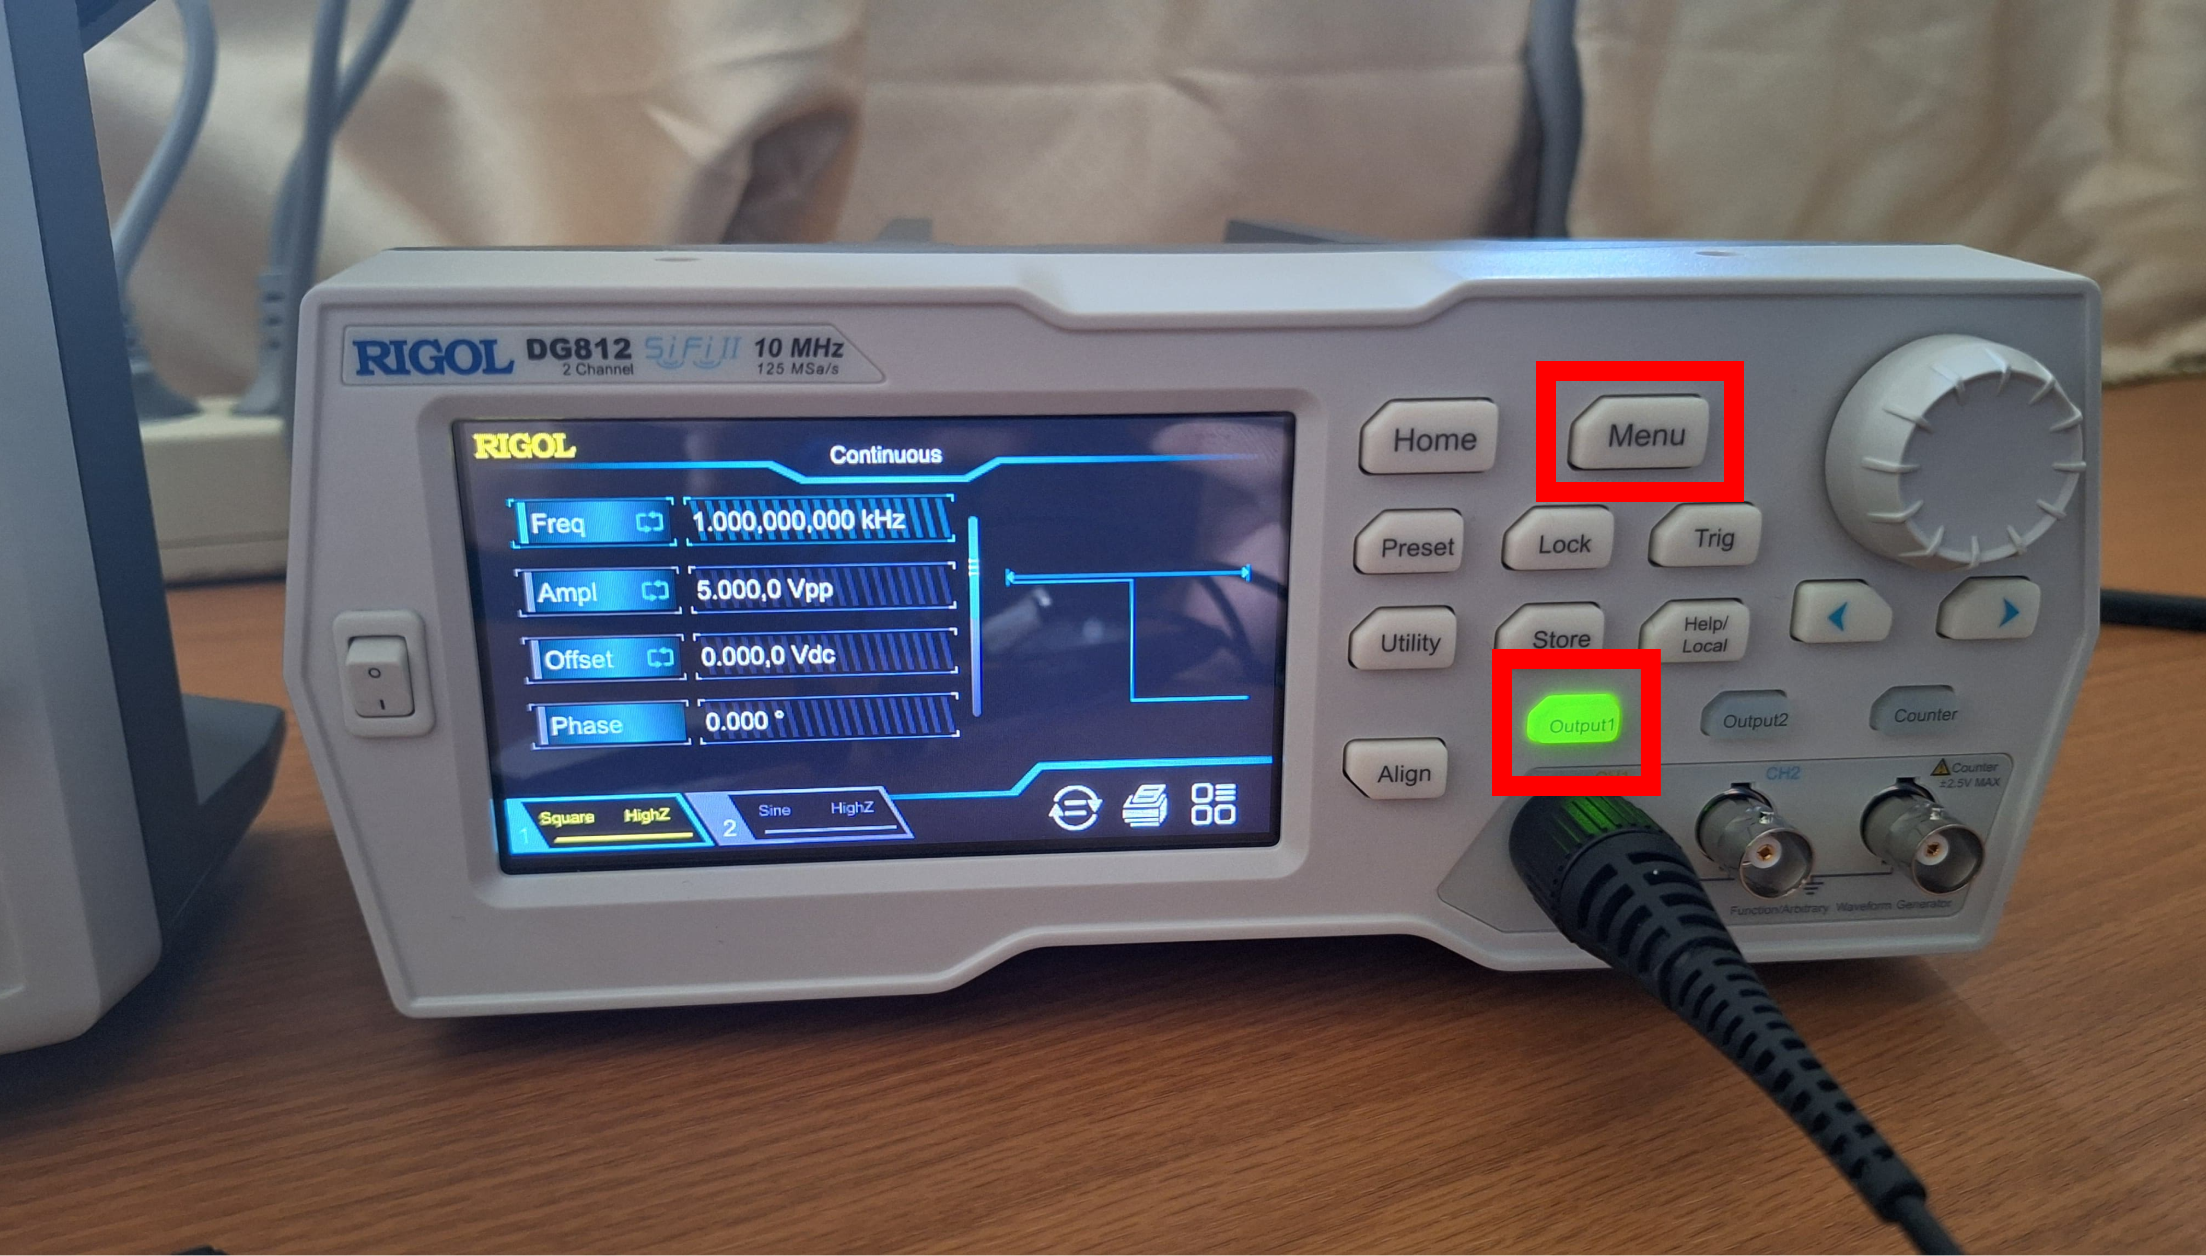
\includegraphics[width=0.7\linewidth]{P1/img/per 2/step 9.png}
			      \caption{Step 9}
			      \label{fig:Step 9(Group 14)}
		      \end{figure}

		\item Tekan AUTO maka sinyal akan ditampilkan melalui osiloskop.
		      \begin{figure}[H]
			      \centering
			      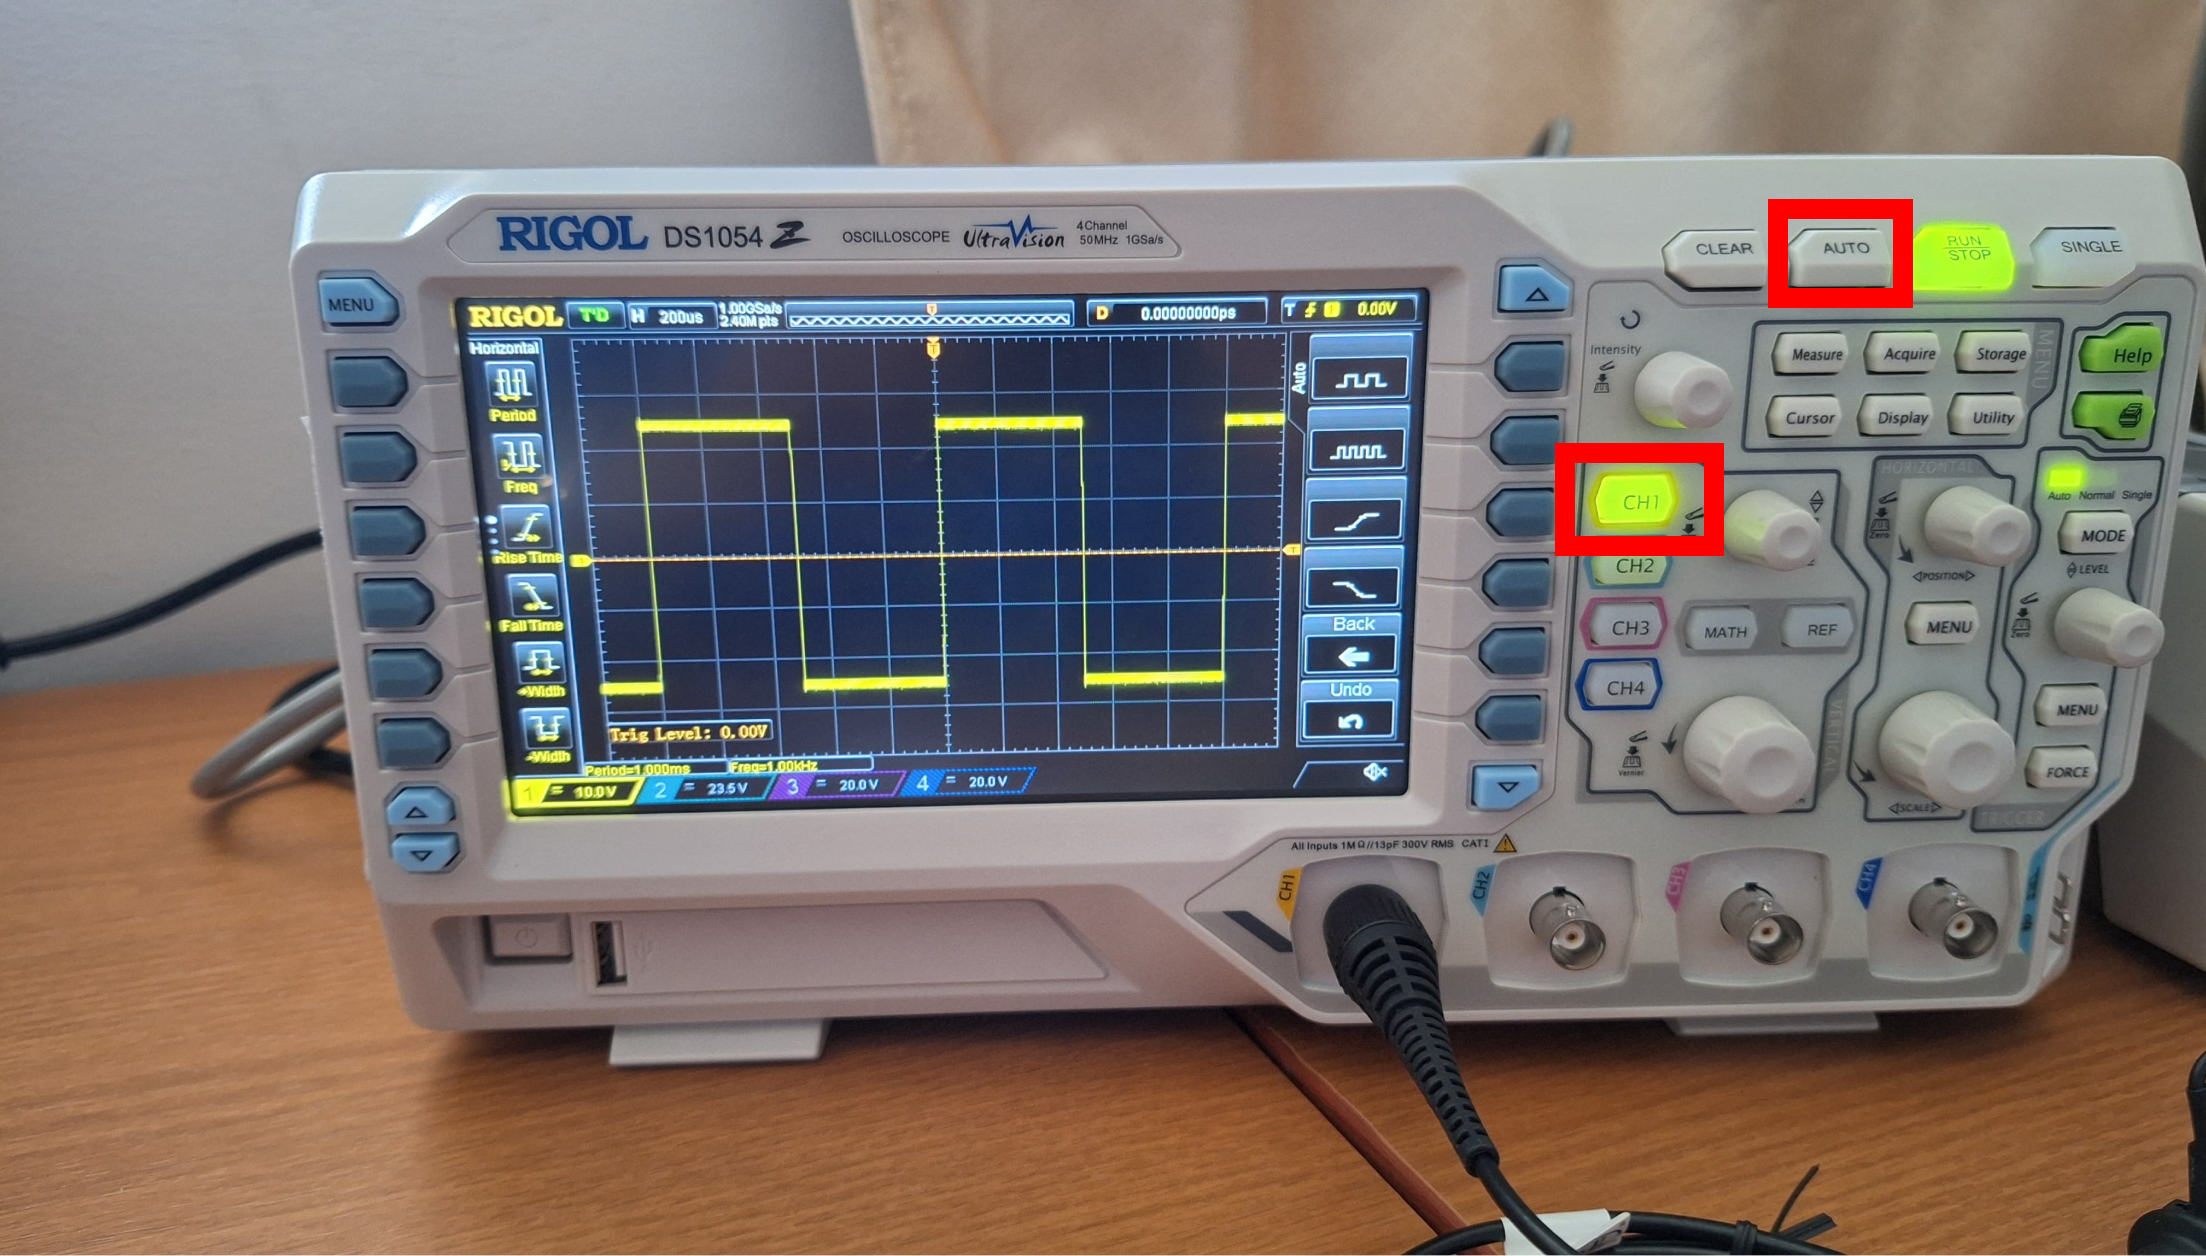
\includegraphics[width=0.7\linewidth]{P1/img/per 2/step 10.png}
			      \caption{Step 10}
			      \label{fig:Step 10(Group 15)}
		      \end{figure}

		\item Lakukanlah kembali untuk menampilkan sinyal arbitary dan sinyal segitiga.
	\end{enumerate}

\end{center}


%===========================================================%
\section{Hasil yang didapat}
Memahami dan mengkonfigurasi Osiloskop dan Function generator dengan tepat.

%===========================================================%
\section{Kesimpulan}
Dengan memahami dan mengkonfigurasi osiloskop dan function generator, kita dapat
\\memahami output sinyal yang ditampilkan oleh osiloskop.

% \section{Pendahuluan}
\subsection{Latar Belakang}
Pada modul kedua ini, kita akan membahas perbandingan hasil (ADC) analog to digital converter pada Arduino dan Osiloskop.Analog to Digital Converter (ADC) adalah perangkat yang berfungsi untuk mengubah sinyal analog menjadi sinyal digital. 
Sinyal analog adalah sinyal yang memiliki nilai yang berubah-ubah dalam waktu, sedangkan sinyal digital adalah sinyal yang memiliki nilai yang berubah-ubah dalam waktu tetapi hanya memiliki dua nilai, yaitu 0 dan 1.
\\\\
ADC umumnya menggunakan metode Successive Approximation Register (SAR) atau metode lainnya untuk mengkonversi sinyal analog menjadi sinyal digital. 
Misalnya, pada Arduino, ADC menggunakan metode SAR untuk mengkonversi tegangan analog menjadi nilai digital yang dapat diproses oleh mikrokontroler.
\\\\
Pada modul praktikum, praktikan menggunakan Arduino untuk membaca tegangan analog dan mengkonversinya menjadi nilai digital menggunakan ADC. 
Sementara itu, osiloskop digunakan untuk memvisualisasikan sinyal listrik dan membandingkan hasil konversi ADC dengan sinyal aslinya.
\\\\

\subsection{Maksud dan Tujuan}
Mengetahui dan membandingkan hasil dari analog to digital converter pada Arduino dan Osiloskop.

\subsection{Hasil yang diharapkan}
Mendapatkan kesimpulan perbandingan hasil analog to digital converter pada Arduino dan Osiloskop.
%===========================================================%
\section{Tugas Pendahuluan}


\begin{center}
	\colorbox{cyan!30}{\parbox{0.8\linewidth}{
		\begin{enumerate}
		\item Buatlah topologi jaringan percobaan 1, 2, dan 3!
		\item Perbedaan Static Routing dan Dynamic Routing.
		\item Keuntungan dan kekurangan Static Routing dan Dynamic Routing
	\end{enumerate}
	}}
\end{center}

%===========================================================%
\section{Alat dan Bahan}
\begin{itemize}[label=$\bullet$, itemsep=-1pt, leftmargin=*]
	\item 1 Perangkat Arduino
	\item 1 Laptop
	\item 1 Osiloskop
	\item 1 Function Generator
	\item Software Arduino IDE
\end{itemize}

%===========================================================%
\section{Jangka Waktu Pelaksanaan}
Pemahaman dan konfigurasi 1 jam.

%===========================================================%
\section{Penjelasan dan Tahapan Konfigurasi}

%======================PERCOBAAN 1==========================%
\subsection{Percobaan 1}
\begin{center}

	\textbf{Memulai Arduino IDE}
	\begin{enumerate}
		\item Hubungkan Arduino Uno dengan laptop.
		\begin{figure}[H]
			\centering
			\includegraphics[width=0.8\linewidth]{P2/img/per1/step 1.png}
			\caption{Step 1}
			\label{fig:Step 1(Step 1)}
		\end{figure}
		\item Buka software Arduino IDE, lalu pilih new sketch.
		\begin{figure}[H]
			\centering
			\includegraphics[width=0.8\linewidth]{P2/img/per1/step 2.png}
			\caption{Step 2}
			\label{fig:Step 2(Step 2)}
		\end{figure}
		\item Buka menu Tools, lalu cek Board dan Port yang terhubung apakah sudah benar
		\\(Port bergantung pada device, jadi bisa berbeda dengan port di Modul).
		\begin{figure}[H]
			\centering
			\includegraphics[width=0.8\linewidth]{P2/img/per1/step 3.png}
			\caption{Step 3}
			\label{fig:Step 3(Step 3)}
		\end{figure}

		\begin{figure}[H]
			\centering
			\includegraphics[width=0.8\linewidth]{P2/img/per1/step 4.png}
			\caption{Step 4}
			\label{fig:Step 4(Step 4)}
		\end{figure}

	\end{enumerate}

	\textbf{Kode Program Arduino}
	\begin{enumerate}
		\item Masukkan kode program dibawah ini untuk menjalankan ADC (Analog to Digital Converter) pada Arduino IDE.
		\begin{figure}[H]
			\centering
			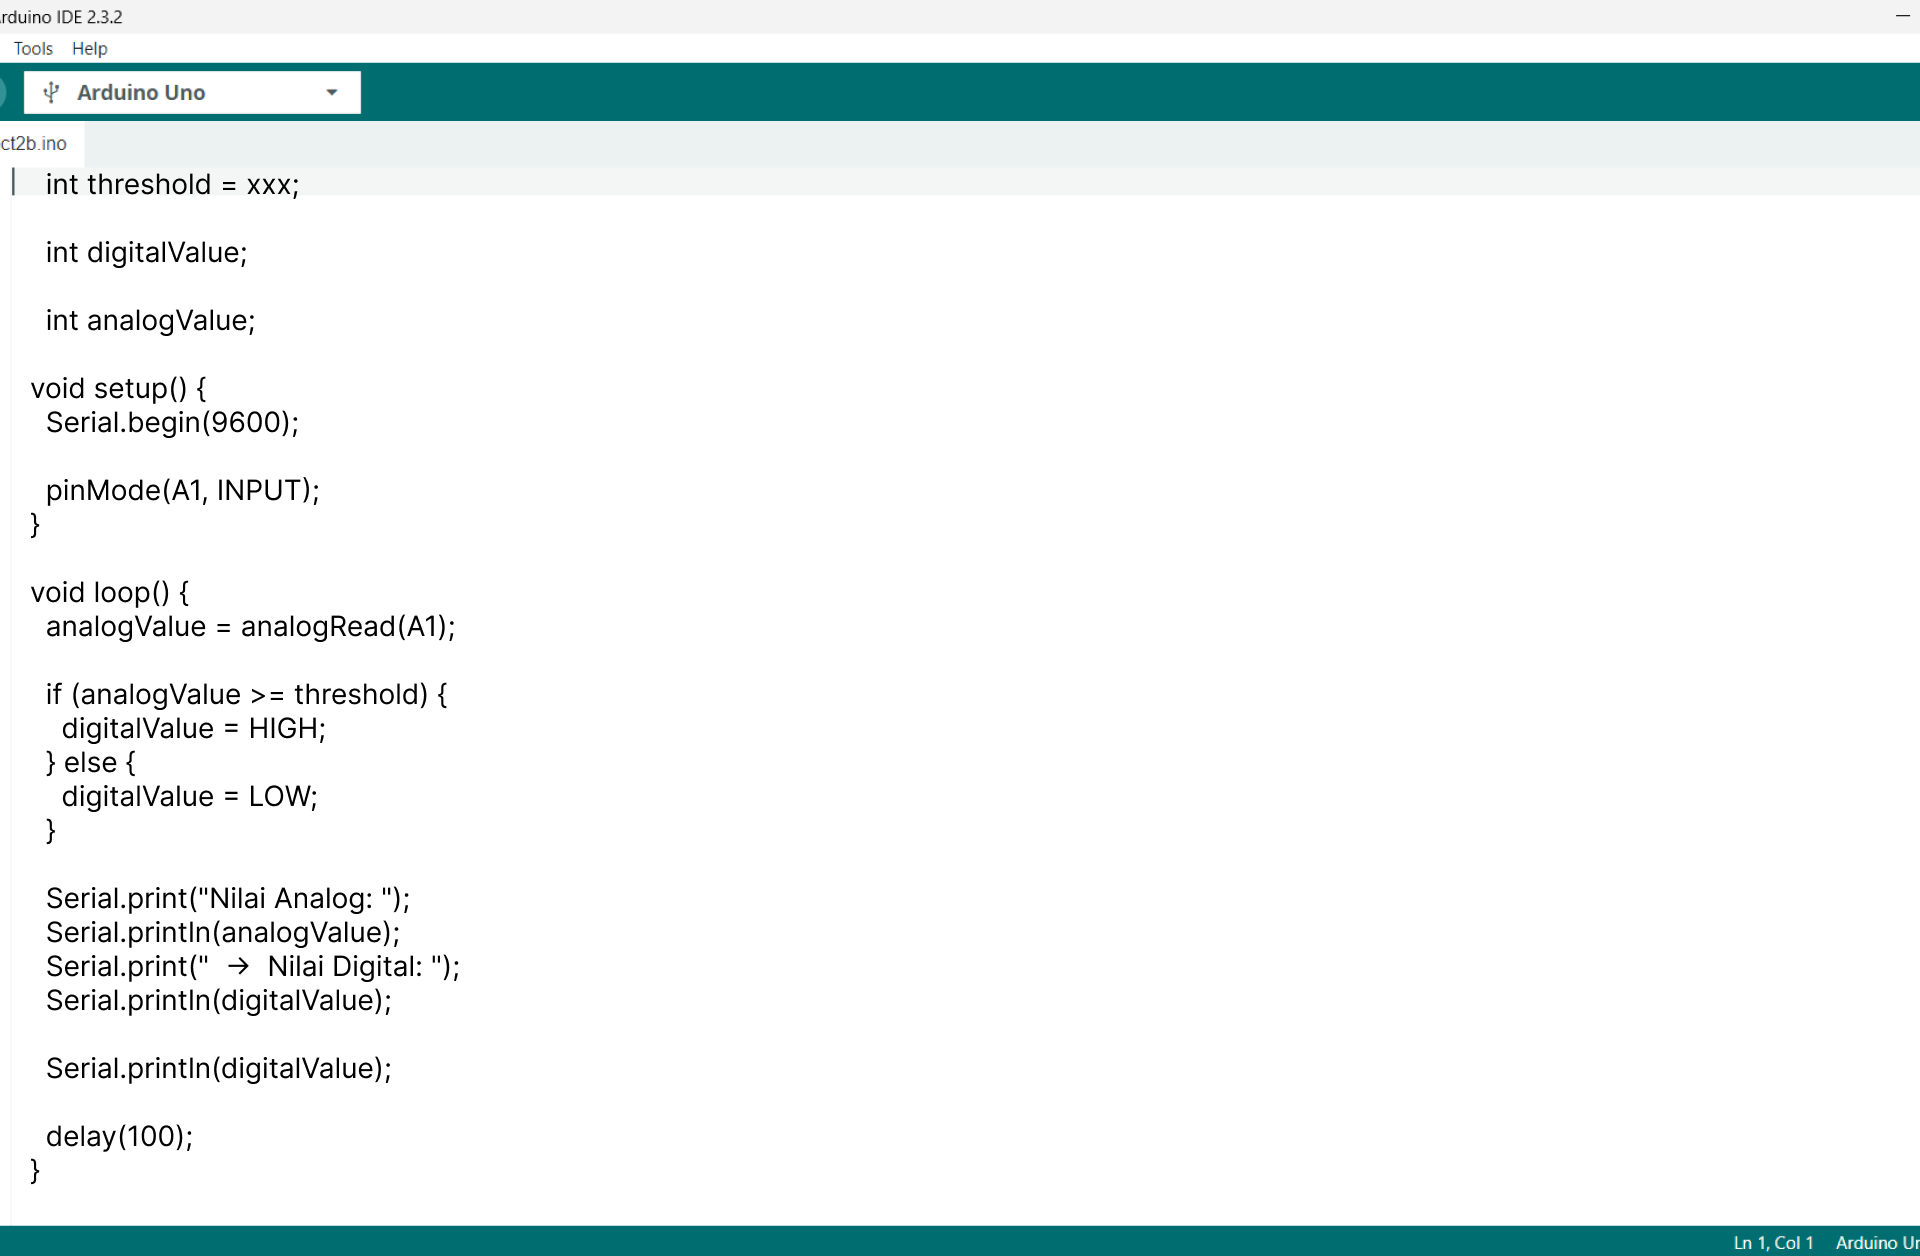
\includegraphics[width=0.8\linewidth]{P2/img/per1/step 5.png}
			\caption{Step 5}
			\label{fig:Step 5(Step 5)}
		\end{figure}

		\item Klik verify, apabila berhasil maka klik upload.
		\begin{figure}[H]
			\centering
			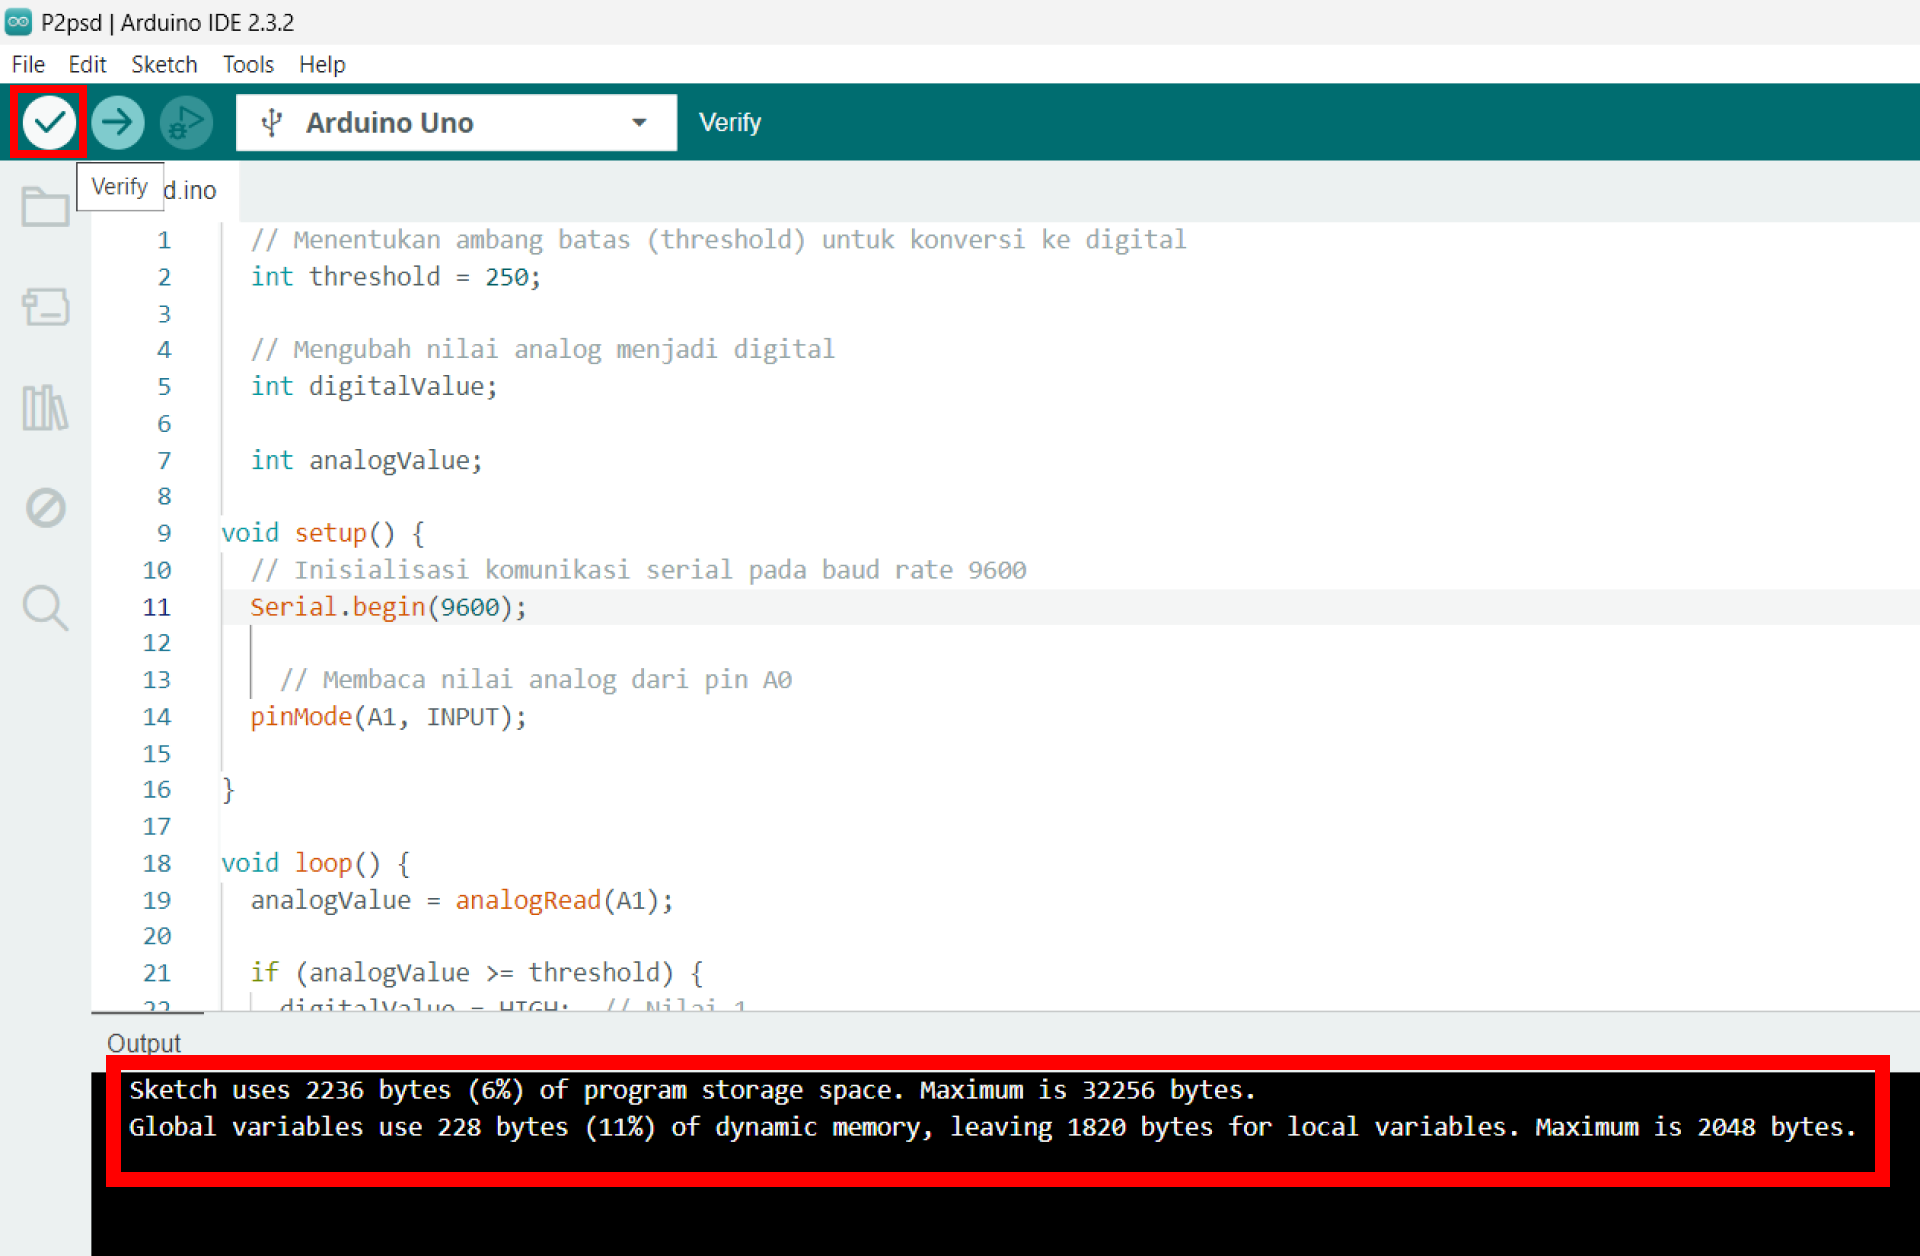
\includegraphics[width=0.8\linewidth]{P2/img/per1/step 6.png}
			\caption{Step 6}
			\label{fig:Step 6(Step 6)} 
		\end{figure}

		\item Klik upload, bisa terlihat done uploading di pojok kanan bawah. 
		\begin{figure}[H]
			\centering
			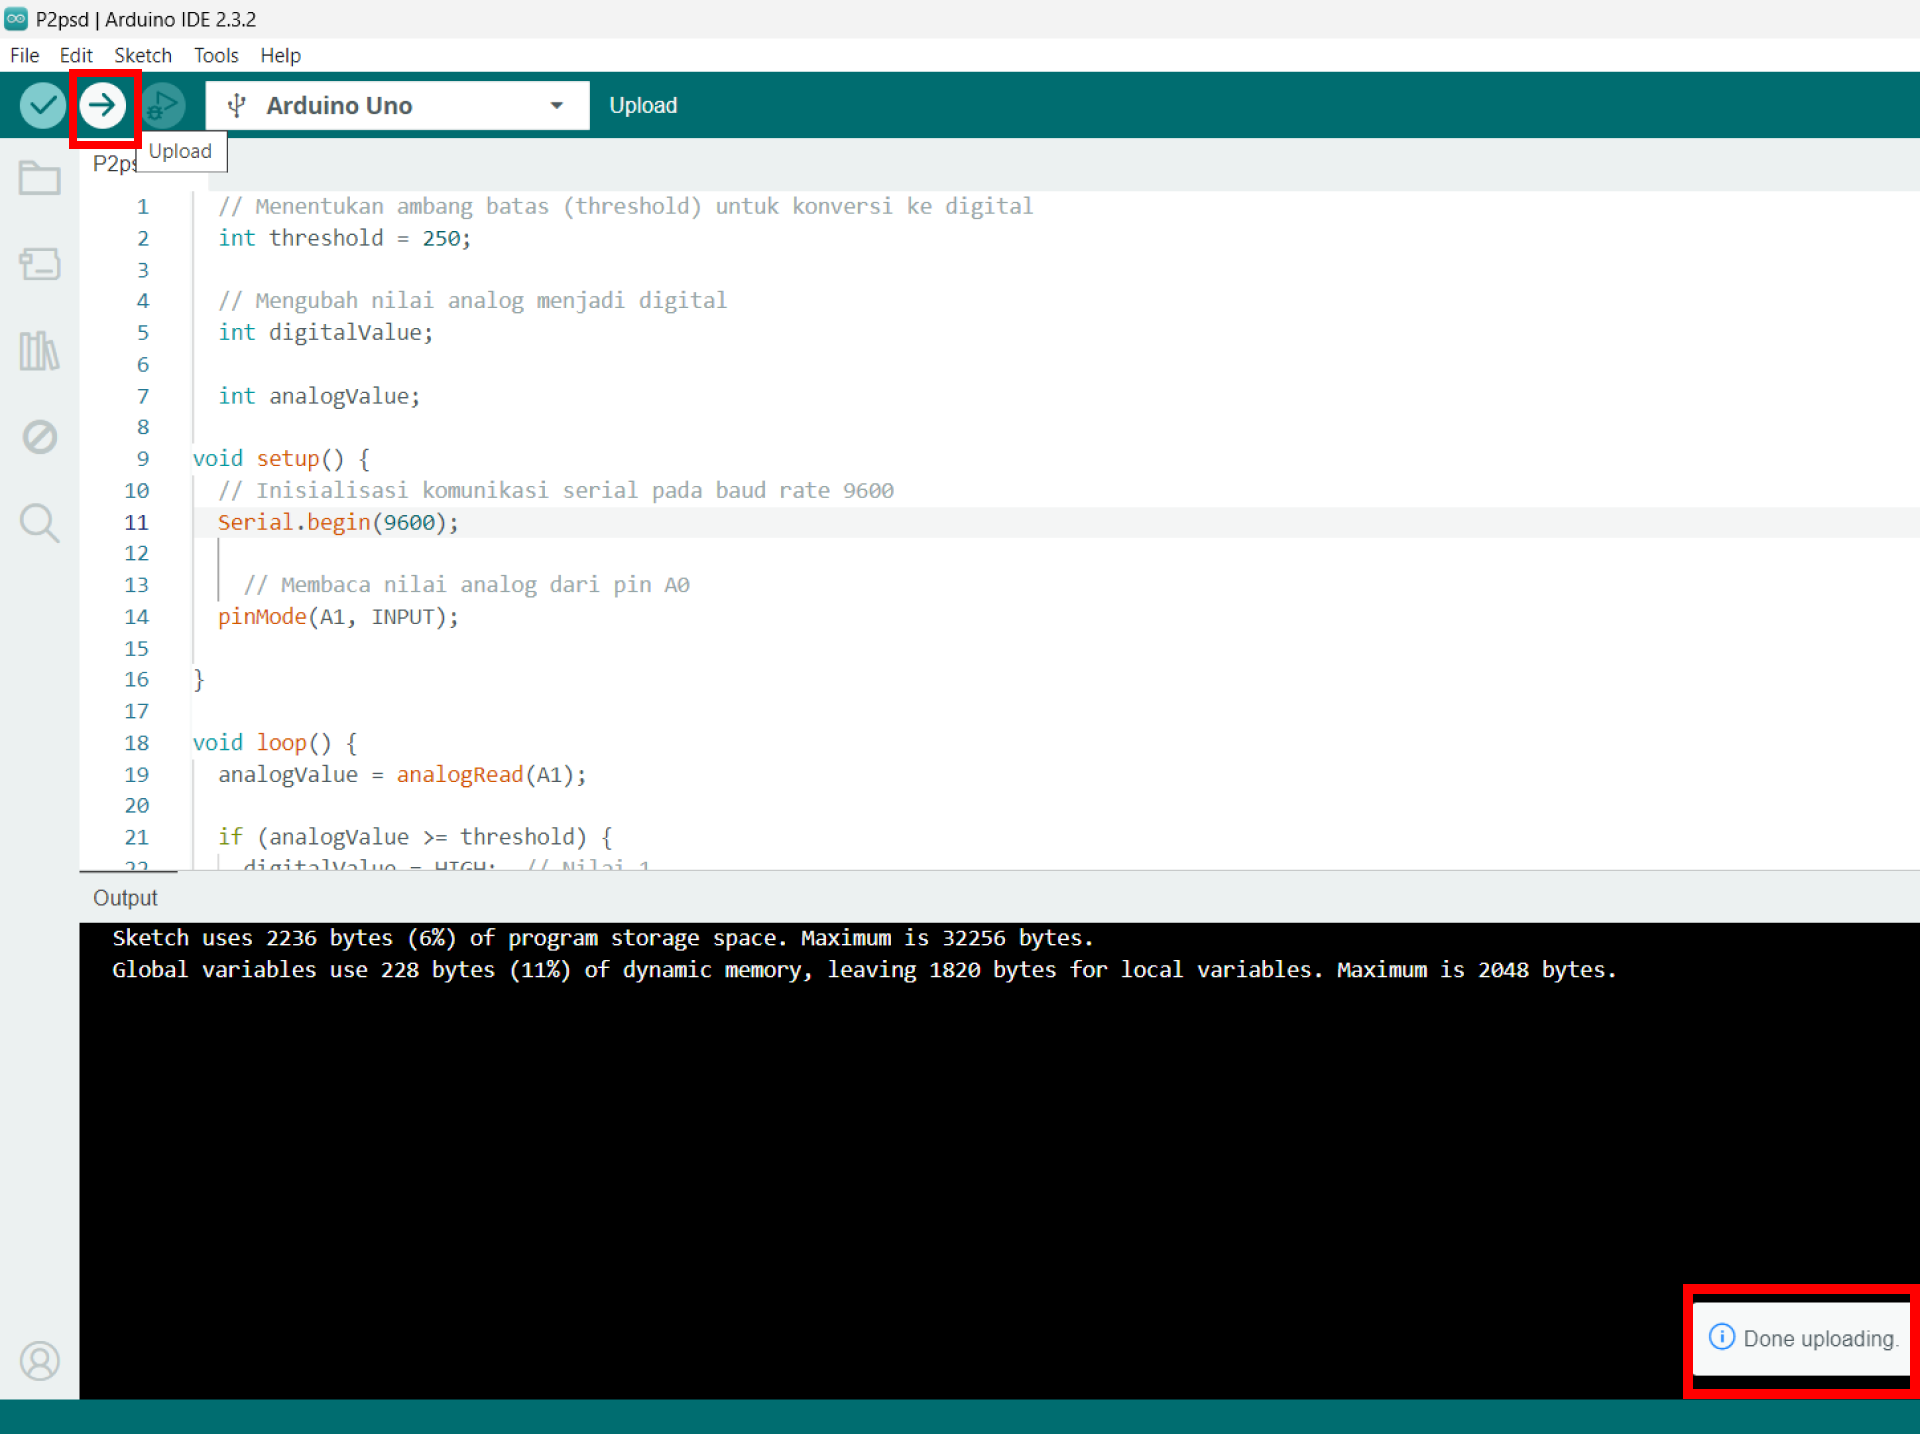
\includegraphics[width=0.8\linewidth]{P2/img/per1/step 7.png}
			\caption{Step 7}
			\label{fig:Step 7(Step 7)} 
		\end{figure}
	\end{enumerate}

	\textbf{Memulai Function Generator}
	\begin{enumerate}
		\item Klik tombol power, untuk menyalakan function generator.
		\begin{figure}[H]
			\centering
			\includegraphics[width=0.8\linewidth]{P2/img/per1/step 8.png}
			\caption{Step 8}
			\label{fig:Step 8(Step 8)}
		\end{figure}

		\item Konfigurasi sinyal input pada Function generator.
		\begin{figure}[H]
			\centering
			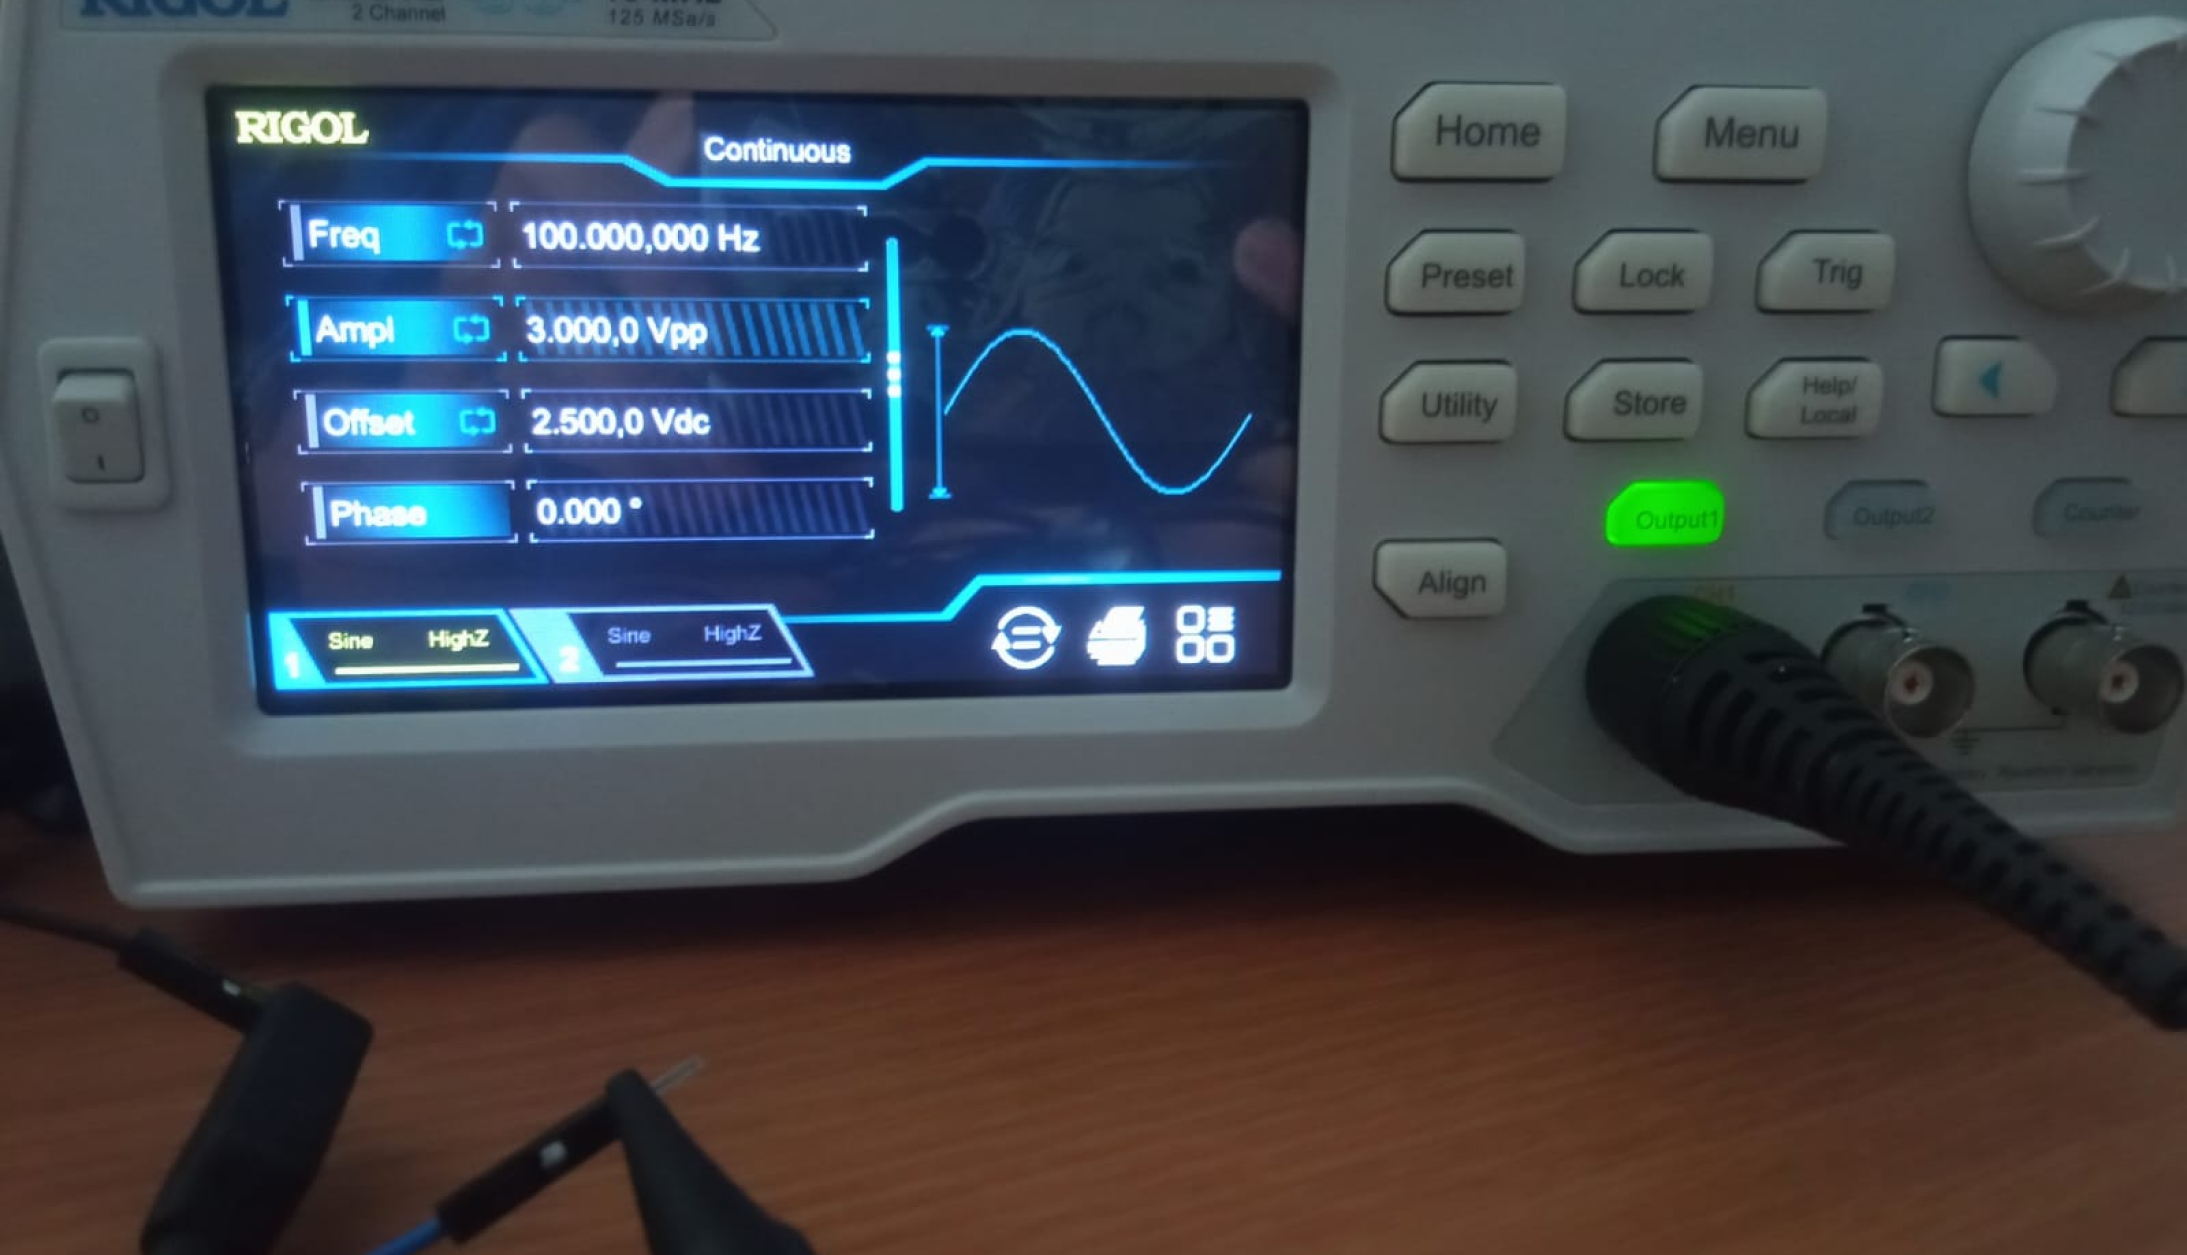
\includegraphics[width=0.8\linewidth]{P2/img/per1/step 9.png}
			\caption{Step 9}
			\label{fig:Step 9(Step 9)}
		\end{figure}
	\end{enumerate}

	\textbf{Konfigurasi Arduino}
	\begin{enumerate}
		\item Hubungkan kabel jumper ke salah satu pin Analog Arduino, kemudian hubungan ke probe.
		\\pengait (positif) Function generator.
		\begin{figure}[H]
			\centering
			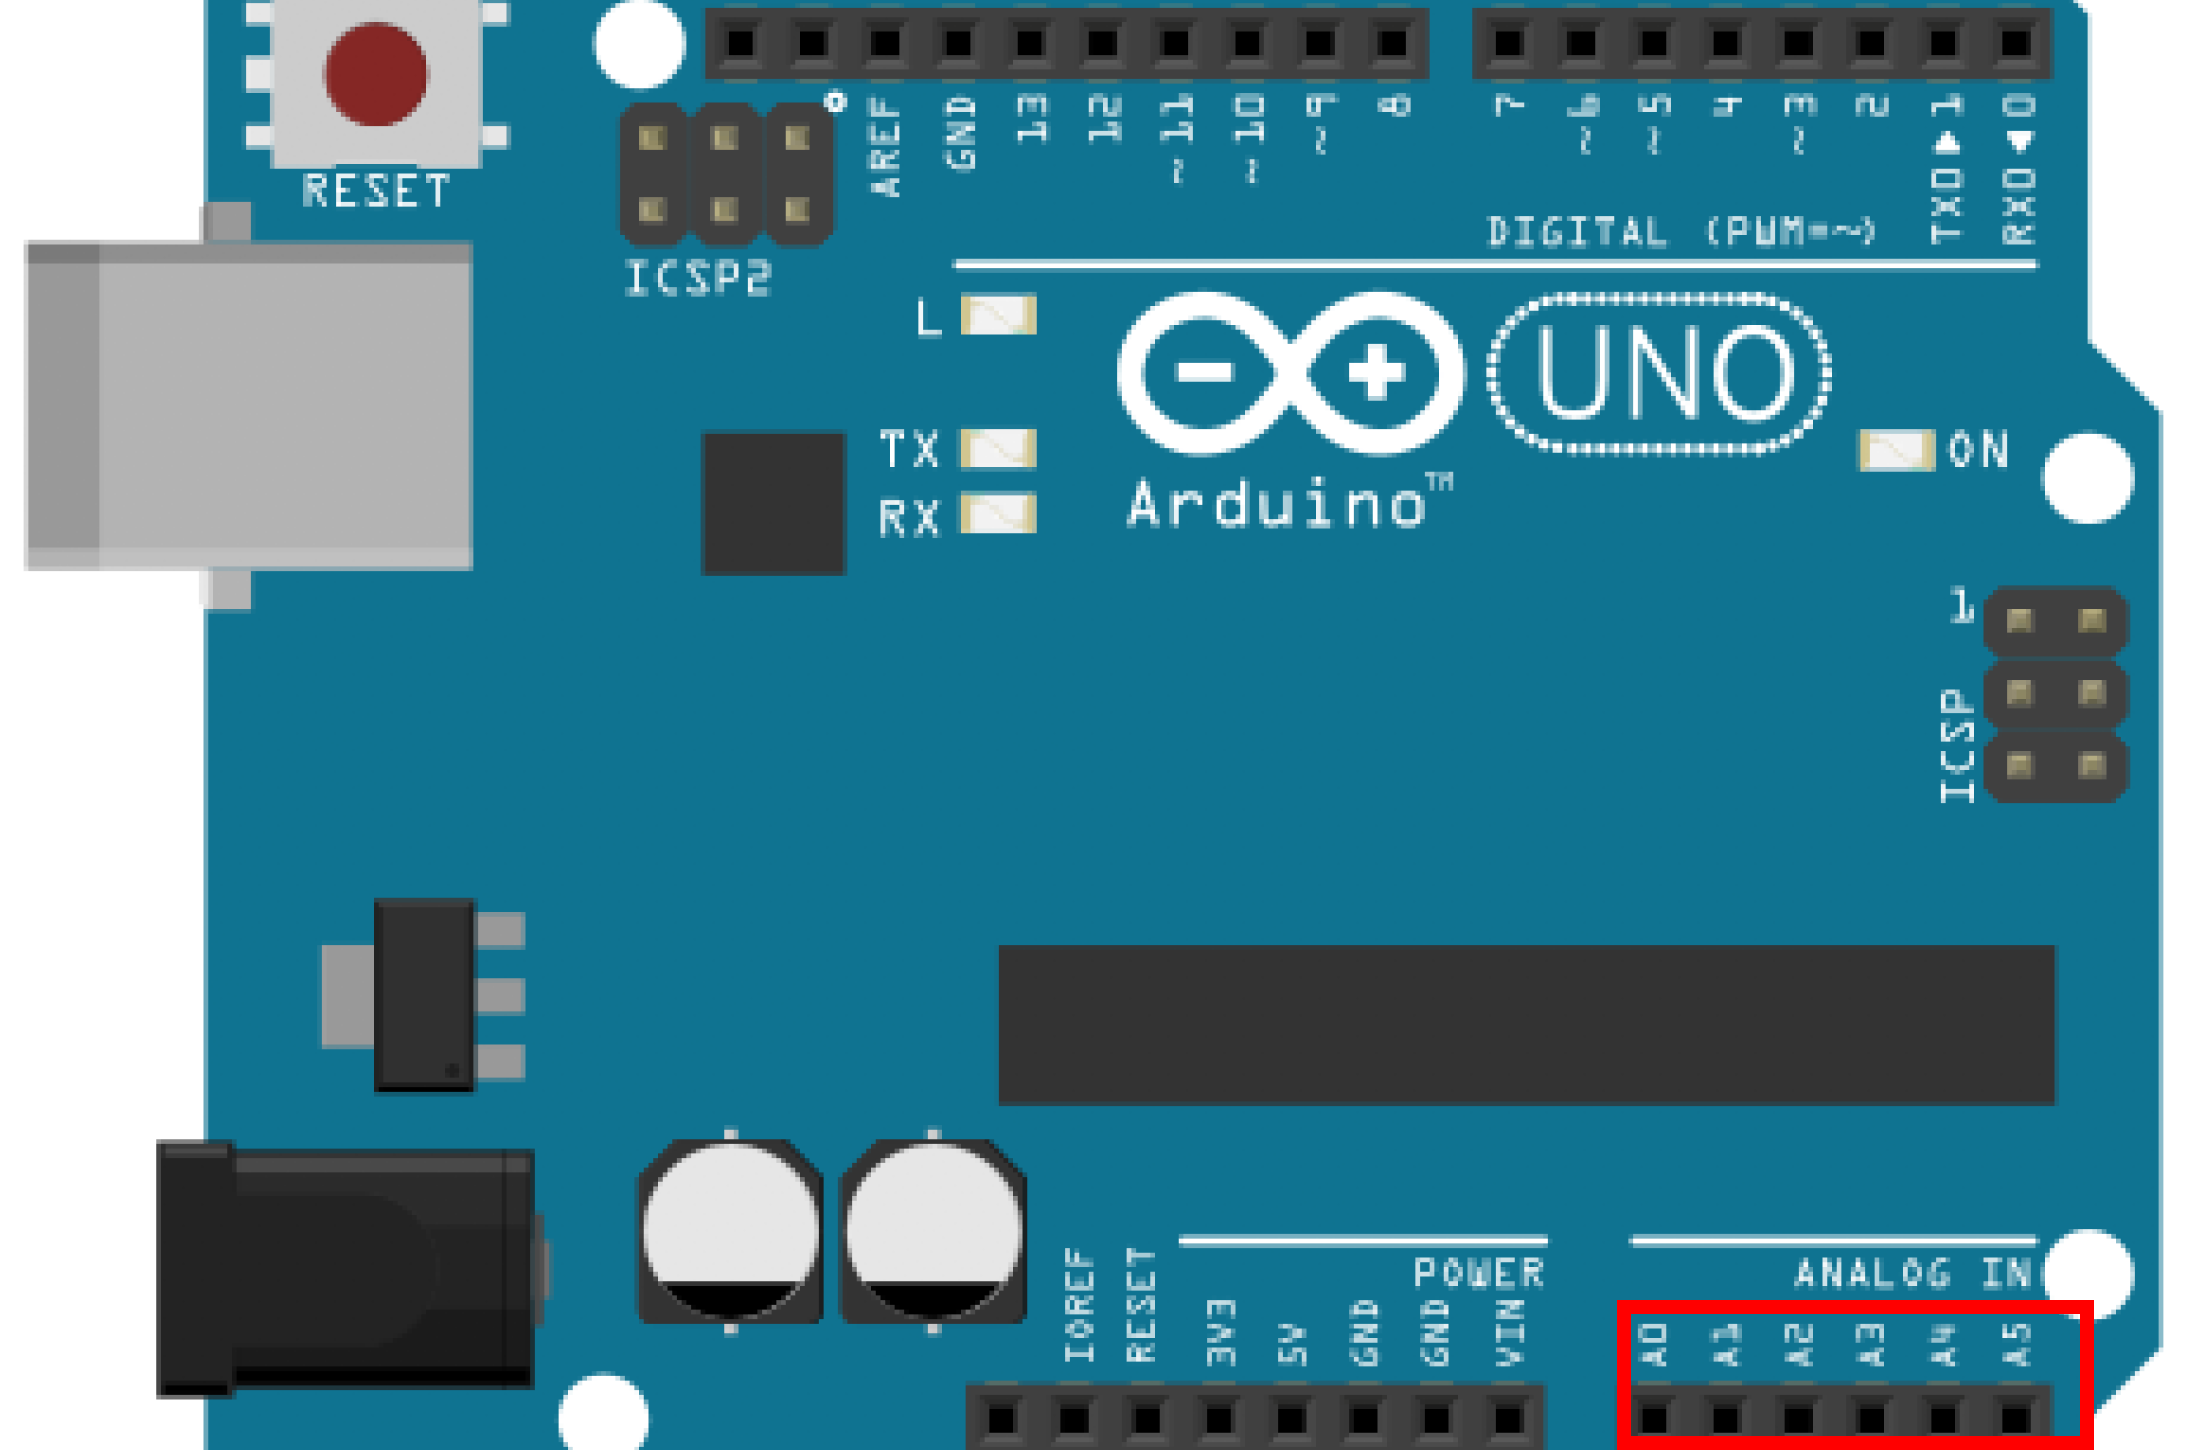
\includegraphics[width=0.8\linewidth]{P2/img/per1/step 10.png}
			\caption{Step 10}
			\label{fig:Step 8(Step 10)}
		\end{figure}

		\item Hubungkan kabel jumper ke salah satu pin GND Arduino, kemudian hubungkan probe.
		\\penjepit buaya (negatif) Function generator.
		\begin{figure}[H]
			\centering
			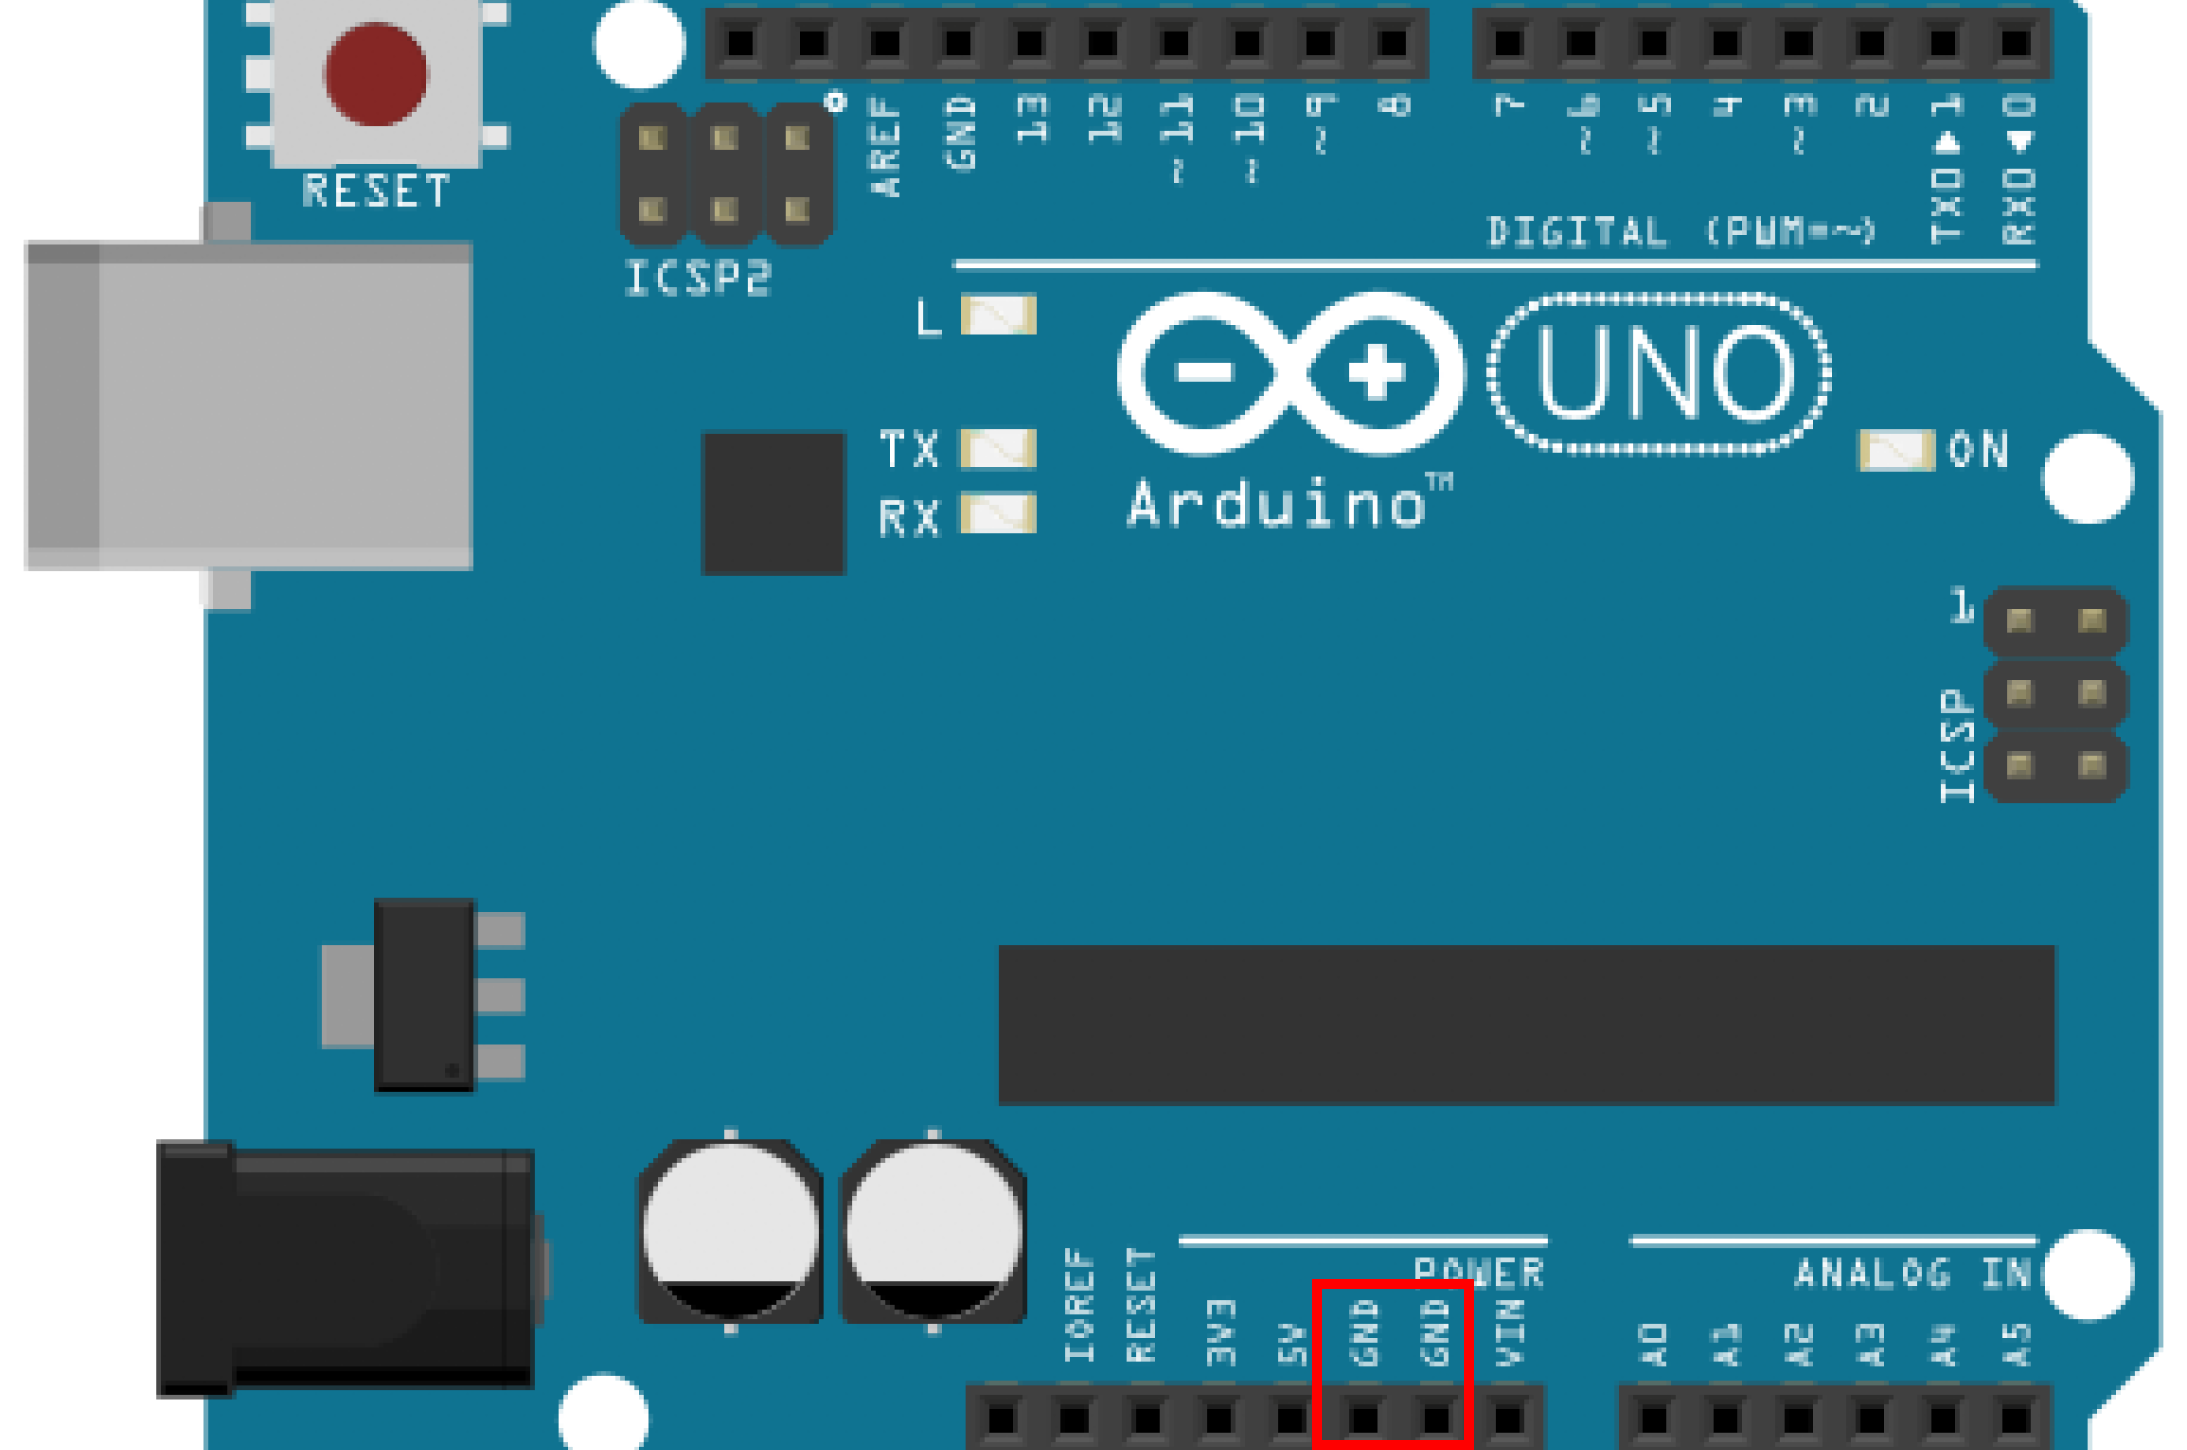
\includegraphics[width=0.8\linewidth]{P2/img/per1/step 11.png}
			\caption{Step 11}
			\label{fig:Step 11(Step 11)}
		\end{figure}

		\item Nyalakan Output 1 pada Function Generator.
		\item Buka Serial plotter di pojok kanan atas pada Arduino IDE.
		\item Buka Serial Monitor di pojok kanan atas pada Arduino IDE.
	\end{enumerate}

\end{center}

%======================PERCOBAAN 2==========================%
\subsection{Percobaan 2}
\begin{center}
	\textbf{Konfigurasi Osiloskop}
	\begin{enumerate}
		\item Hubungkan kabel power ke osiloskop, lalu tekan tombol power untuk menyalakan Osiloskop. 
		\begin{figure}[H]
			\centering
			\includegraphics[width=0.9\linewidth]{P2/img/per2/step 1.png}
			\caption{Step 1}
			\label{fig:Step 1(Step 1)}
		\end{figure}
		\item Hubungkan kabel probe pada channel 1. 
		\begin{figure}[H]
			\centering
			\includegraphics[width=0.8\linewidth]{P2/img/per2/step 2.png}
			\caption{Step 2}
			\label{fig:Step 2(Step 2)}
		\end{figure}
		\item Hubungkan kabel jumper dari salah satu pin Analog Arduino dengan probe pengait (positif) osiloskop dan function generator.
		\item Hubungkan kabel jumper pin GND Arduino dengan probe penjepit buaya (negatif) osiloskop.
		\item Klik AUTO pada Osiloskop.
		\item Bandingkan hasil sinyal yang ditampilkan oleh Serial plotter Arduino dengan Osiloskop.
	\end{enumerate}	
\end{center}

%===========================================================%
\section{Hasil yang didapat}
Memahami perbedaan hasil sinyal digital yang diperoleh oleh Arduino dan Osiloskop.

%===========================================================%
\section{Kesimpulan}
Mengetahui hasil sinyal manakah yang lebih baik dihasilkan dari kedua perangkat \\Arduino dan Osiloskop. 



% \section{Pendahuluan}
\subsection{Latar Belakang}
Digital to Analog Converter (DAC) adalah perangkat yang berfungsi untuk mengubah sinyal digital menjadi sinyal analog. 
Sinyal digital yang dihasilkan oleh komputer atau mikrokontroler Arduino harus dapat diubah menjadi sinyal analog untuk dapat digunakan dalam berbagai aplikasi, seperti penggunaan dalam sistem audio, pengukuran, dan lain-lain.
\\\\
Prinsip kerja DAC melibatkan proses penggunaan resistor yang berat sebelah (binary weighted resistors) atau jaringan resistor R-2R ladder untuk menghasilkan output analog yang sesuai dengan input digital. 
Metode ini memungkinkan DAC untuk menghasilkan sinyal analog yang akurat dengan menggunakan kombinasi bit-bit digital.
\\\\
Dalam sistem monitoring, DAC digunakan untuk mengubah sinyal digital dari sensor menjadi sinyal analog yang dapat diproses oleh sistem. 
Misalnya, dalam pengukuran suhu, sensor suhu menghasilkan sinyal digital yang kemudian dikonversi menjadi sinyal analog oleh DAC sebelum diproses oleh sistem. 
Hal ini menunjukkan bahwa DAC sangat penting dalam sistem monitoring untuk mengubah sinyal digital menjadi sinyal analog yang dapat diproses oleh komputer.
\\\\

\subsection{Maksud dan Tujuan}
Mengetahui dan membandingkan hasil dari digital to analog converter pada Arduino dan Osiloskop.

\subsection{Hasil yang diharapkan}
Mendapatkan kesimpulan perbandingan hasil digital to analog converter pada Arduino dan Osiloskop.
%===========================================================%
\section{Tugas Pendahuluan}
\begin{center}
	\colorbox{cyan!30}{\parbox{0.8\linewidth}{
    \begin{enumerate}
        \item Apa yang dimaksud dengan Simple Queue?
        \item Keuntungan apa yang bisa didapat jika diterapkan ke suatu network?
    \end{enumerate}}}
\end{center}

%===========================================================%
\section{Alat dan Bahan}
\begin{itemize}[label=$\bullet$, itemsep=-1pt, leftmargin=*]
	\item 1 Perangkat Osiloskop
	\item 1 Laptop
	\item 1 Arduino
	\item Software Arduino IDE
\end{itemize}

%===========================================================%
\section{Jangka Waktu Pelaksanaan}
Pemahaman dan konfigurasi 1 jam.

%===========================================================%
\section{Penjelasan dan Tahapan Konfigurasi}

%======================PERCOBAAN 1==========================%
\subsection{Percobaan 1}
\begin{center}
	\textbf{Memulai Arduino IDE}
    \begin{enumerate}
        \item Buka aplikasi Arduino IDE.
        \item Masukkan kode program untuk menjalankan DAC (Digital to Analog Converter) pada Arduino IDE.
        \begin{figure}[H]
			\centering
			\includegraphics[width=0.8\linewidth]{P3/img/step 1.png}
			\caption{Step 1}
			\label{fig:Step 1}
		\end{figure}
		\item Hubungkan Arduino Uno dengan Arduino IDE.
        \begin{figure}[H]
			\centering
			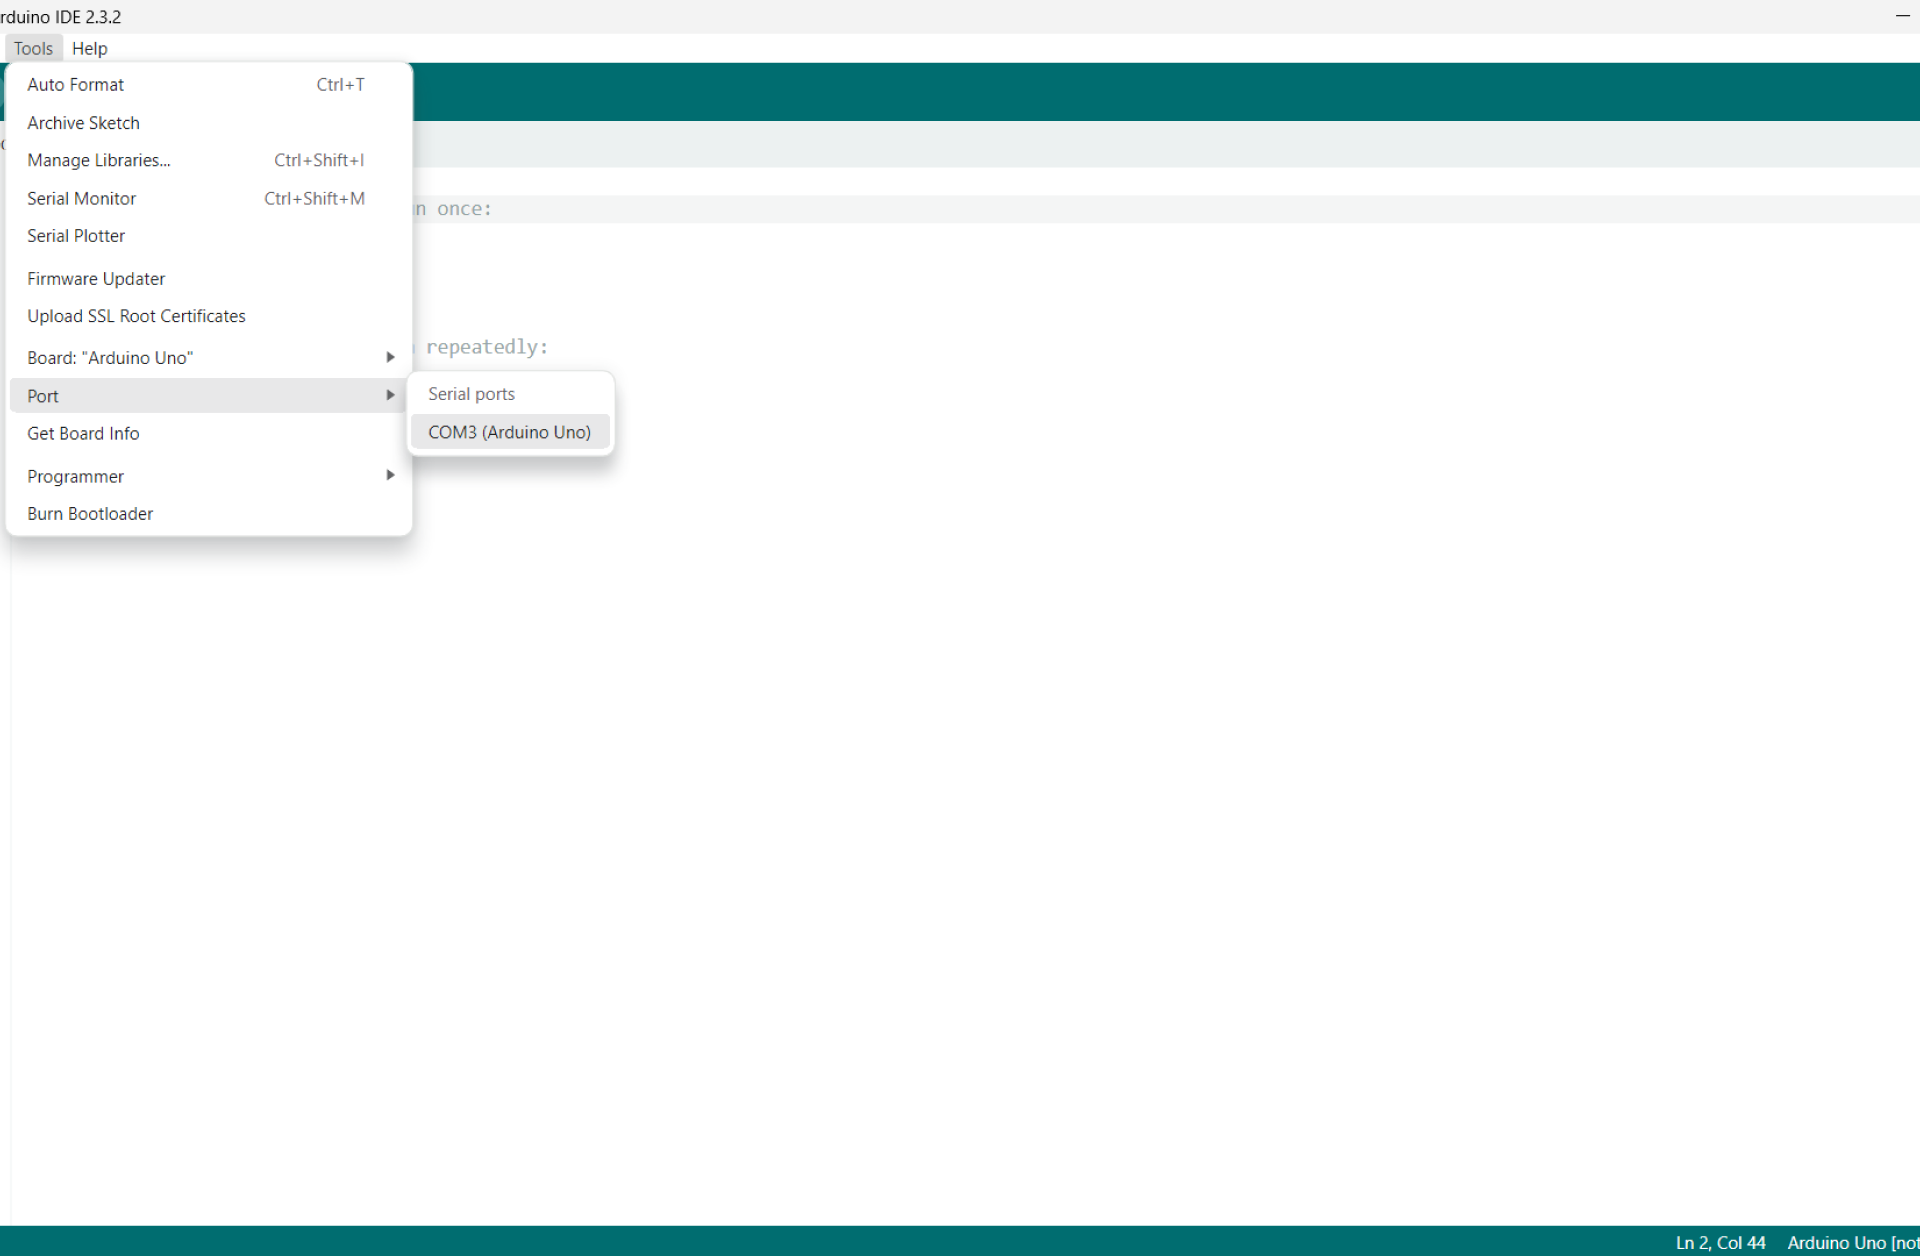
\includegraphics[width=0.8\linewidth]{P3/img/step 2.png}
			\caption{Step 2}
			\label{fig:Step 2}
		\end{figure}
        \item Buat rangkaian Arduino Uno dengan R2R Ladder seperti gambar dibawah ini.
        \begin{figure}[H]
			\centering
			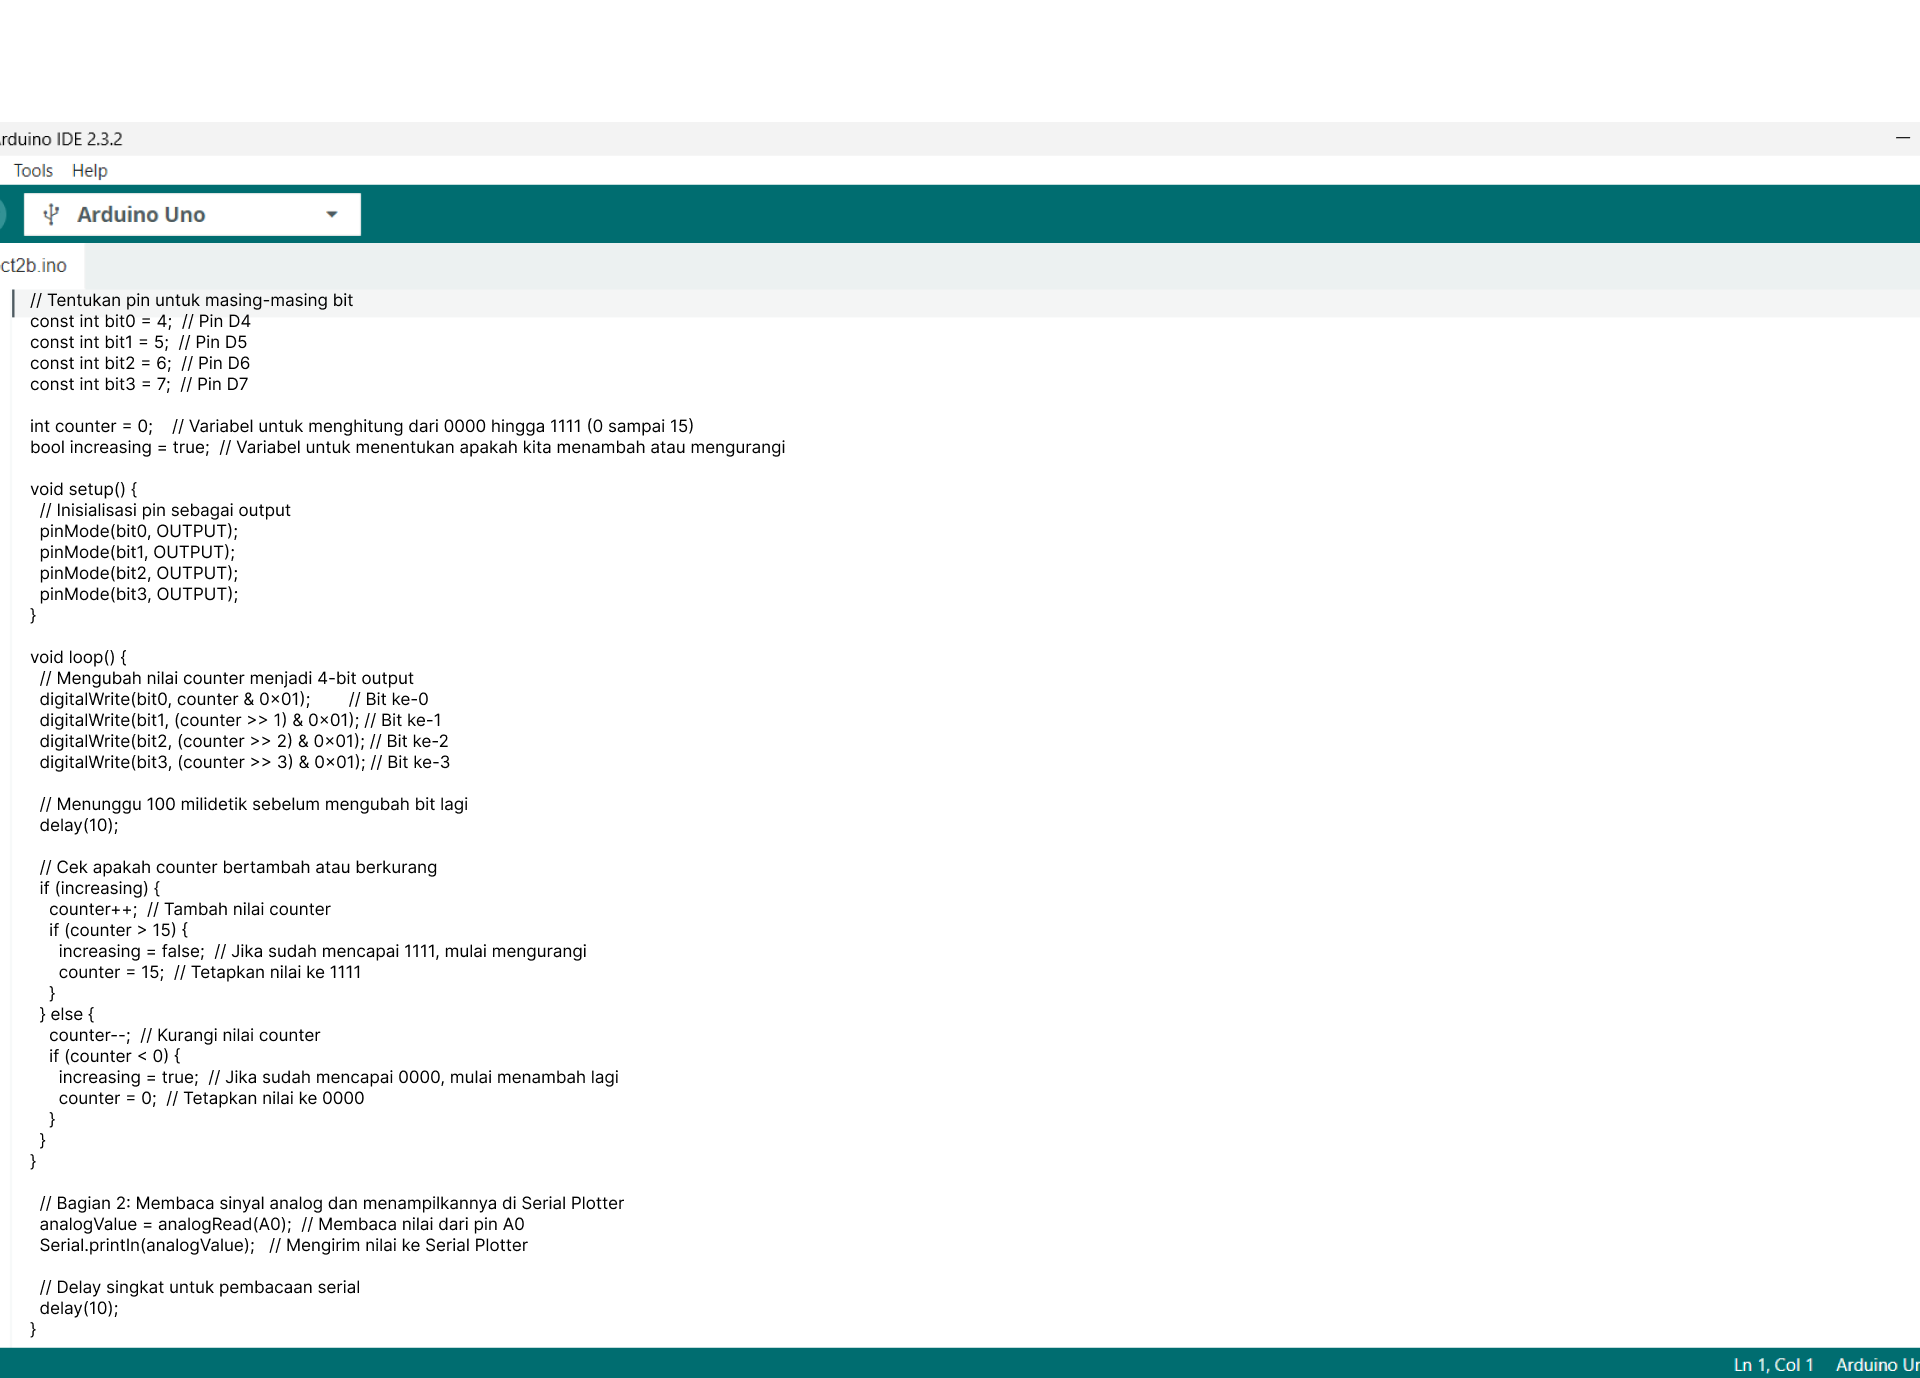
\includegraphics[width=0.8\linewidth]{P3/img/Step 3.png}
			\caption{Step 3}
			\label{fig:Step 3}
		\end{figure}
        \item Klik Verify, apabila berhasil maka klik upload.
        \begin{figure}[H]
			\centering
			\includegraphics[width=0.8\linewidth]{P3/img/step 4.png}
			\caption{Step 4}
			\label{fig:Step 4}
		\end{figure}

		\begin{figure}[H]
			\centering
			\includegraphics[width=0.8\linewidth]{P3/img/step 5.png}
			\caption{Step 5}
			\label{fig:Step 5}
		\end{figure}

		\begin{figure}[H]
			\centering
			\includegraphics[width=0.8\linewidth]{P3/img/step 6.png}
			\caption{Step 6}
			\label{fig:Step 5}
		\end{figure}

        \item Buka Serial Plotter di pojok kanan atas pada Arduino IDE.
        \item Buka Serial Monitor di pojok kanan atas pada Arduino IDE.

    \end{enumerate}
\end{center}

\subsection{Percobaan 2}
\begin{center}
	\textbf{Konfigurasi Osiloskop}
	\begin{enumerate}
		\item Hubungkan kabel power ke osiloskop, lalu tekan tombol power untuk menyalakan Osiloskop. 
		\begin{figure}[H]
			\centering
			\includegraphics[width=0.8\linewidth]{P3/img/step 7.png}
			\caption{Step 1}
			\label{fig:Step 1(Step 1)}
		\end{figure}
		\item Hubungkan kabel probe pada channel 1. 
		\begin{figure}[H]
			\centering
			\includegraphics[width=0.8\linewidth]{P3/img/step 8.png}
			\caption{Step 2}
			\label{fig:Step 2(Step 2)}
		\end{figure}
		\item Hubungkan kabel output R2R Ladder dengan probe pengait osiloskop.
		\item Hubungkan kabel probe penjepit buaya osiloskop pada GND R2R Ladder.
		\item Klik AUTO pada Osiloskop.
		\item Bandingkan hasil sinyal yang ditampilkan oleh Serial plotter Arduino dengan Osiloskop.
	\end{enumerate}	
\end{center}

%===========================================================%
\section{Hasil yang didapat}
Memahami perbedaan hasil sinyal anlog yang diperoleh oleh Arduino dan Osiloskop.

%===========================================================%
\section{Kesimpulan}
Mengetahui hasil sinyal manakah yang lebih baik dihasilkan dari kedua perangkat \\Arduino dan Osiloskop.

% \section{Pendahuluan}
\subsection{Latar Belakang}
Digital filter adalah suatu alat yang digunakan untuk memodifikasi sinyal digital dengan cara menghilangkan atau mengurangi noise, menghilangkan komponen frekuensi tertentu, dan memperbaiki kualitas sinyal. 
Digital filter sangat penting dalam berbagai aplikasi, seperti pengolahan sinyal audio, pengukuran, dan sistem monitoring.
\\\\
Ada dua jenis utama digital filter: Filter Infinite Impulse Response (IIR) dan Filter Finite Impulse Response (FIR).
Filter IIR: Menggunakan konsep feedback dan feed forward untuk menghasilkan output yang berdasarkan input sekarang, input sebelumnya, dan output sebelumnya. Filter IIR dapat memiliki respon frekuensi yang lebih kompleks dan dapat digunakan untuk aplikasi yang memerlukan pengurangan noise yang lebih efektif.
Filter FIR: Menggunakan koefisien yang ditetapkan secara eksplisit untuk menghasilkan output yang berdasarkan input sekarang saja. Filter FIR memiliki respon frekuensi yang lebih sederhana dan lebih mudah untuk dirancang, tetapi dapat lebih efektif dalam menghilangkan noise yang memiliki frekuensi tertentu.
\\\\
Dalam sistem monitoring, digital filter digunakan untuk menghilangkan noise dan memperbaiki kualitas data sensor. 
Misalnya, dalam pengukuran suhu, digital filter digunakan untuk menghilangkan noise yang dapat mempengaruhi akurasi pengukuran suhu. 

\subsection{Maksud dan Tujuan}
Memahami konsep dan aplikasi digital filter pada pengolahan sinyal digital.
\subsection{Hasil yang diharapkan}
Memahami hasil sinyal sebelum dan sesudah dilakukan digital filter.

%===========================================================%
\section{Tugas Pendahuluan}
\begin{center}
	\colorbox{cyan!30}{\parbox{0.8\linewidth}{
    \begin{enumerate}
        \item Apa itu PPTP dan bagaimana cara kerjanya?
        \item Apa kelebihan dan kekurangan dari penggunaan PPTP dibandingkan protokol VPN lainnya seperti L2TP atau OpenVPN?
    \end{enumerate}}}
\end{center}

%===========================================================%
\section{Alat dan Bahan}
\begin{itemize}[label=$\bullet$, itemsep=-1pt, leftmargin=*]
	\item 1 Perangkat Arduino
	\item 1 Laptop
	\item 1 Osiloskop
	\item 1 Function Generator
	\item Software Arduino IDE
\end{itemize}

%===========================================================%
\section{Jangka Waktu Pelaksanaan}
Pemahaman dan konfigurasi 1 jam.

%===========================================================%
\section{Penjelasan dan Tahapan Konfigurasi}

%======================PERCOBAAN 1==========================%
\subsection{Percobaan 1}
\begin{center}

	\textbf{Memulai Arduino IDE}
	\begin{enumerate}
		\item Hubungkan Arduino Uno dengan laptop.
		\begin{figure}[H]
			\centering
			\includegraphics[width=0.8\linewidth]{P4/img/per1/step 1.png}
			\caption{Step 1}
			\label{fig:Step 1(Step 1)}
		\end{figure}
		\item Buka software Arduino IDE, lalu pilih new sketch.
		\begin{figure}[H]
			\centering
			\includegraphics[width=0.8\linewidth]{P4/img/per1/step 2.png}
			\caption{Step 2}
			\label{fig:Step 2(Step 2)}
		\end{figure}
		\item Buka menu Tools, lalu cek Board dan Port yang terhubung apakah sudah benar
		\\(Port bergantung pada device, jadi bisa berbeda dengan port di Modul).
		\begin{figure}[H]
			\centering
			\includegraphics[width=0.8\linewidth]{P4/img/per1/step 3.png}
			\caption{Step 3}
			\label{fig:Step 3(Step 3)}
		\end{figure}
		\begin{figure}[H]
			\centering
			\includegraphics[width=0.8\linewidth]{P2/img/per1/step 4.png}
			\caption{Step 4}
			\label{fig:Step 4(Step 4)}
		\end{figure}
	
	\textbf{Kode Program Arduino}
		\item Masukkan kode program dibawah ini untuk menjalankan Digital Filter pada Arduino IDE.
		\begin{figure}[H]
			\centering
			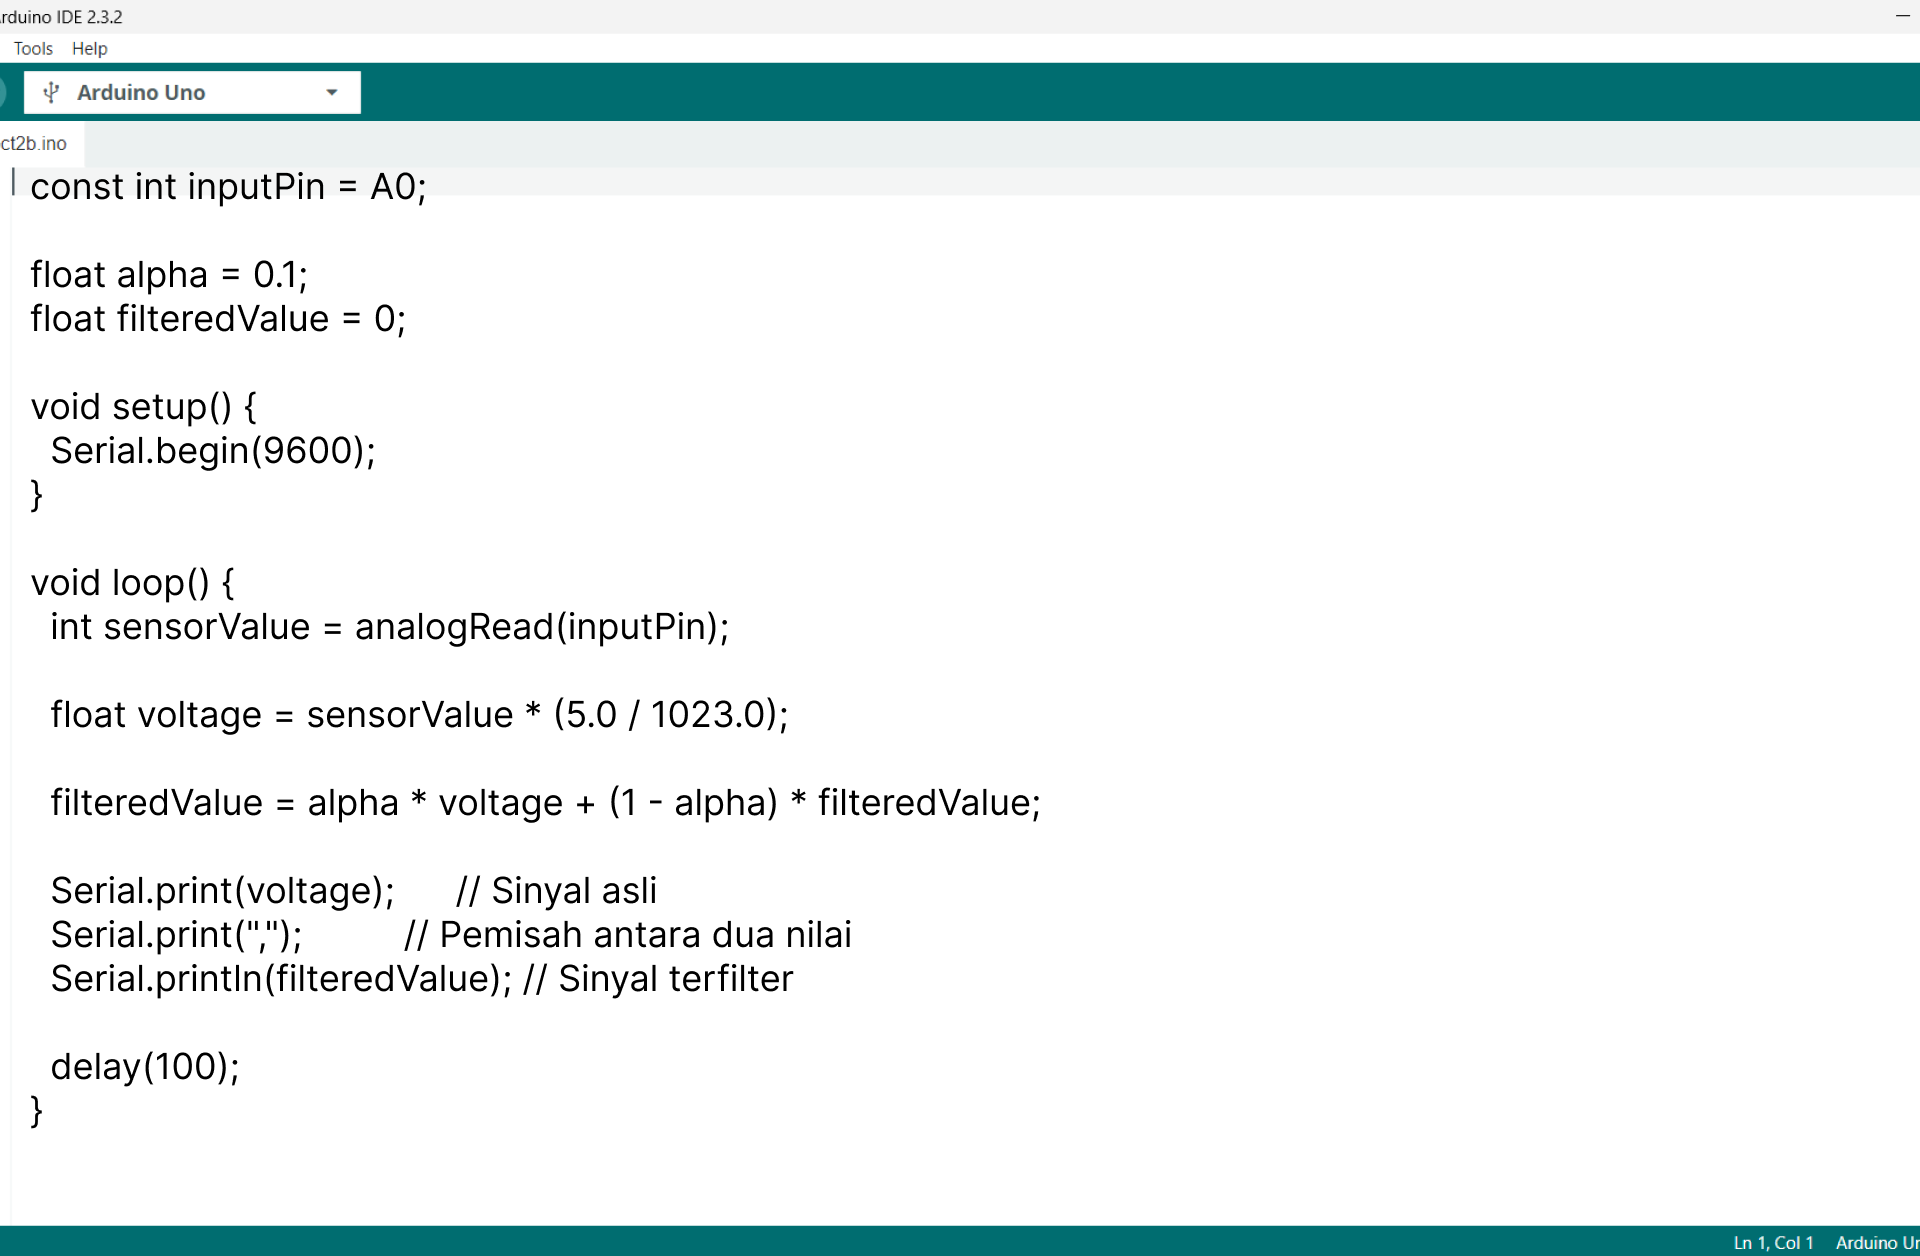
\includegraphics[width=0.8\linewidth]{P4/img/per1/step 5.png}
			\caption{Step 5}
			\label{fig:Step 5(Step 5)}
		\end{figure}
	
		\item Klik verify, apabila berhasil maka klik upload.
	\end{enumerate}
	
	\textbf{Memulai Function Generator}
	\begin{enumerate}
		\item Klik tombol power, untuk menyalakan function generator.
		\begin{figure}[H]
			\centering
			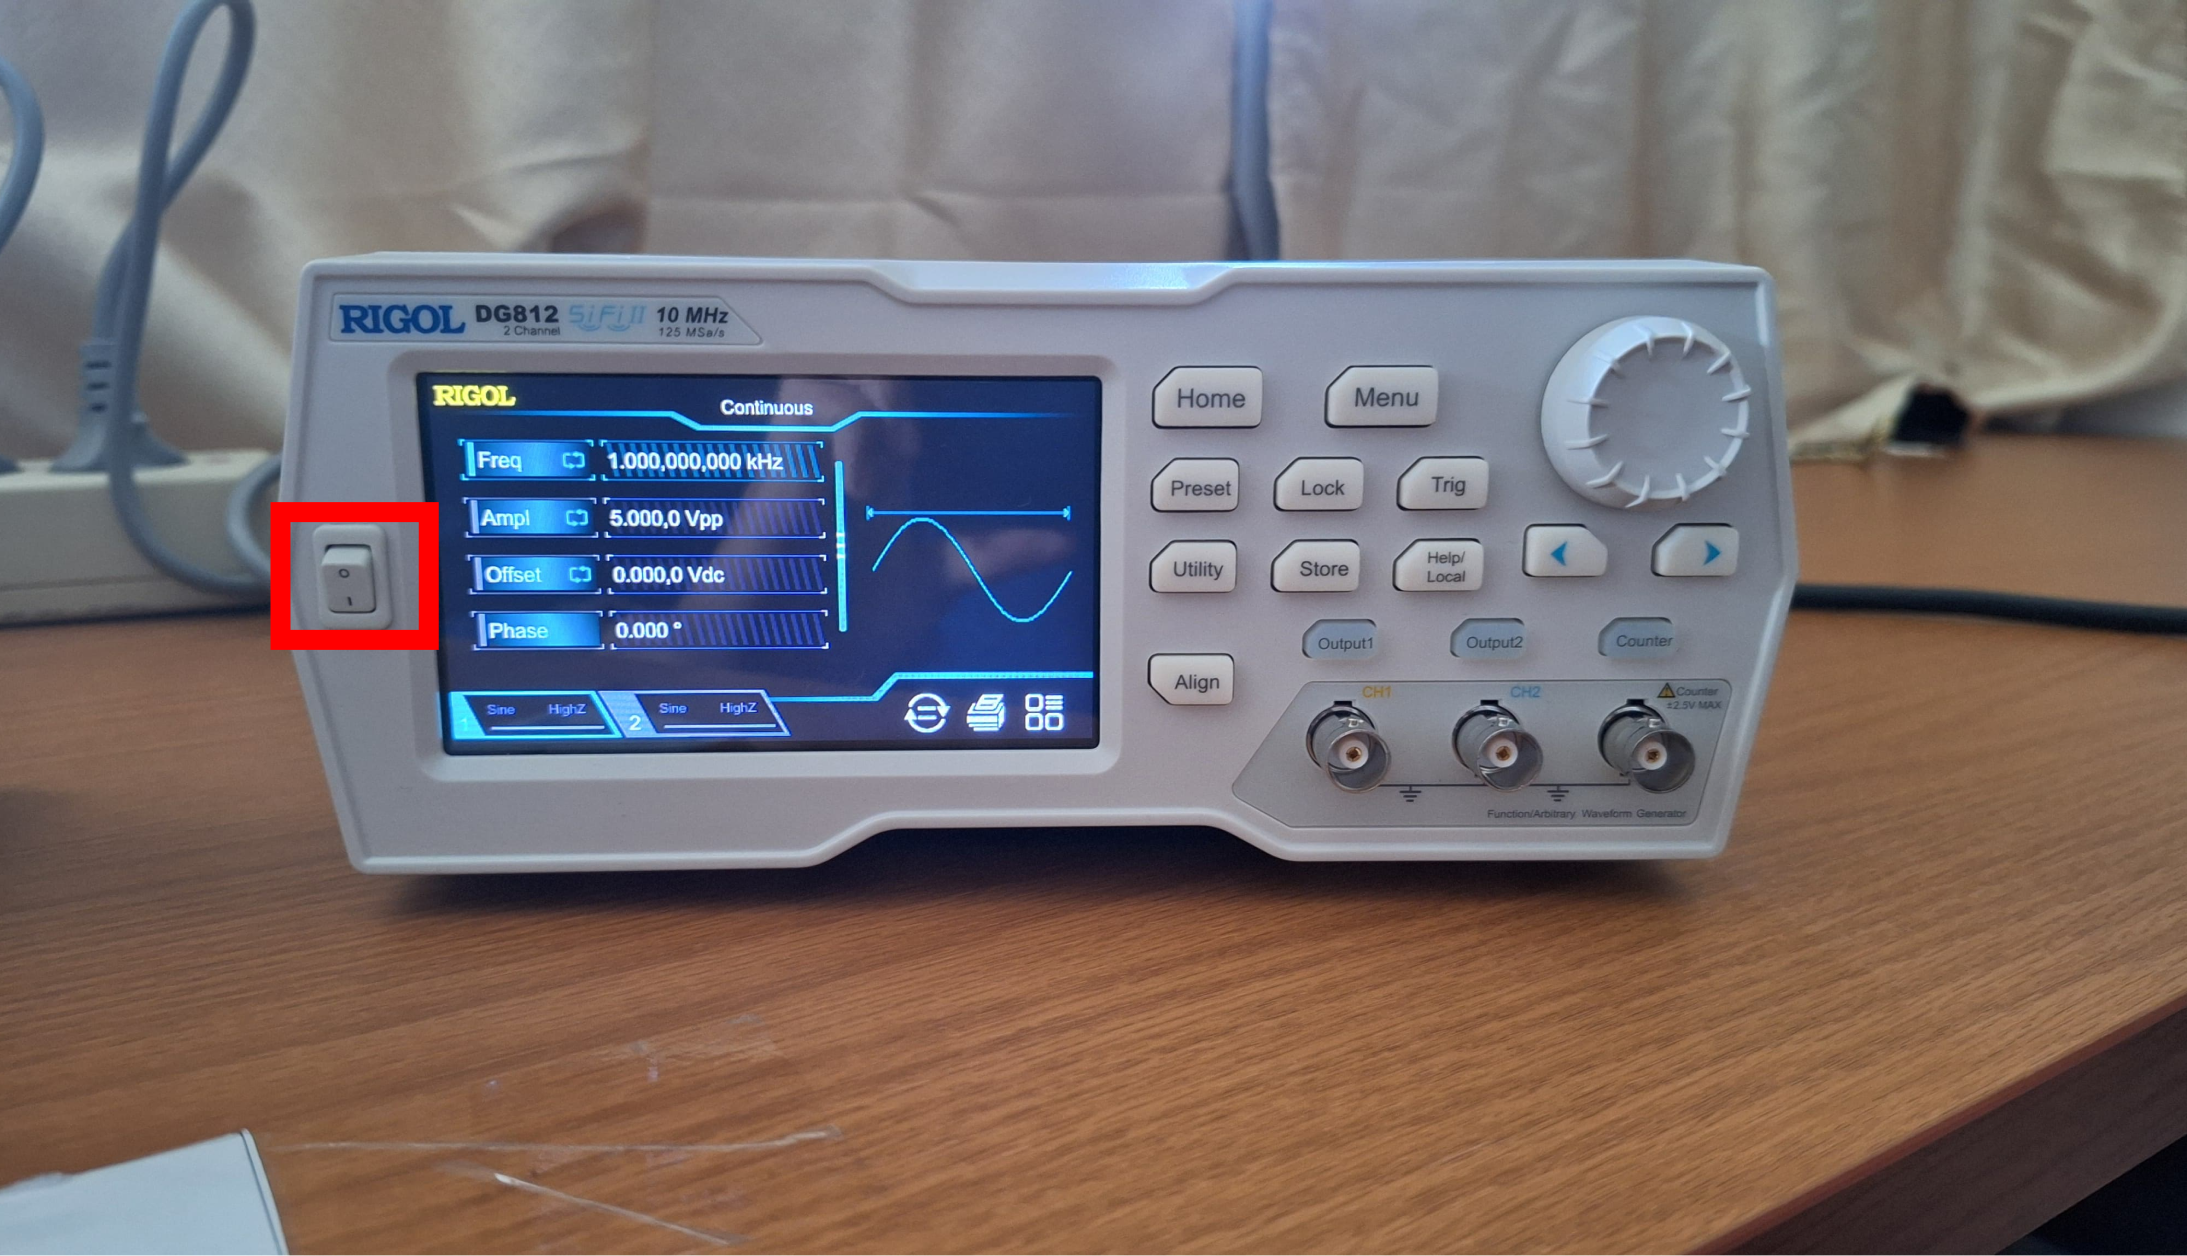
\includegraphics[width=0.8\linewidth]{P4/img/per1/step 6.png}
			\caption{Step 6}
			\label{fig:Step 6(Step 6)}
		\end{figure}

		\item Konfigurasi sinyal input pada Function generator.
		\begin{figure}[H]
			\centering
			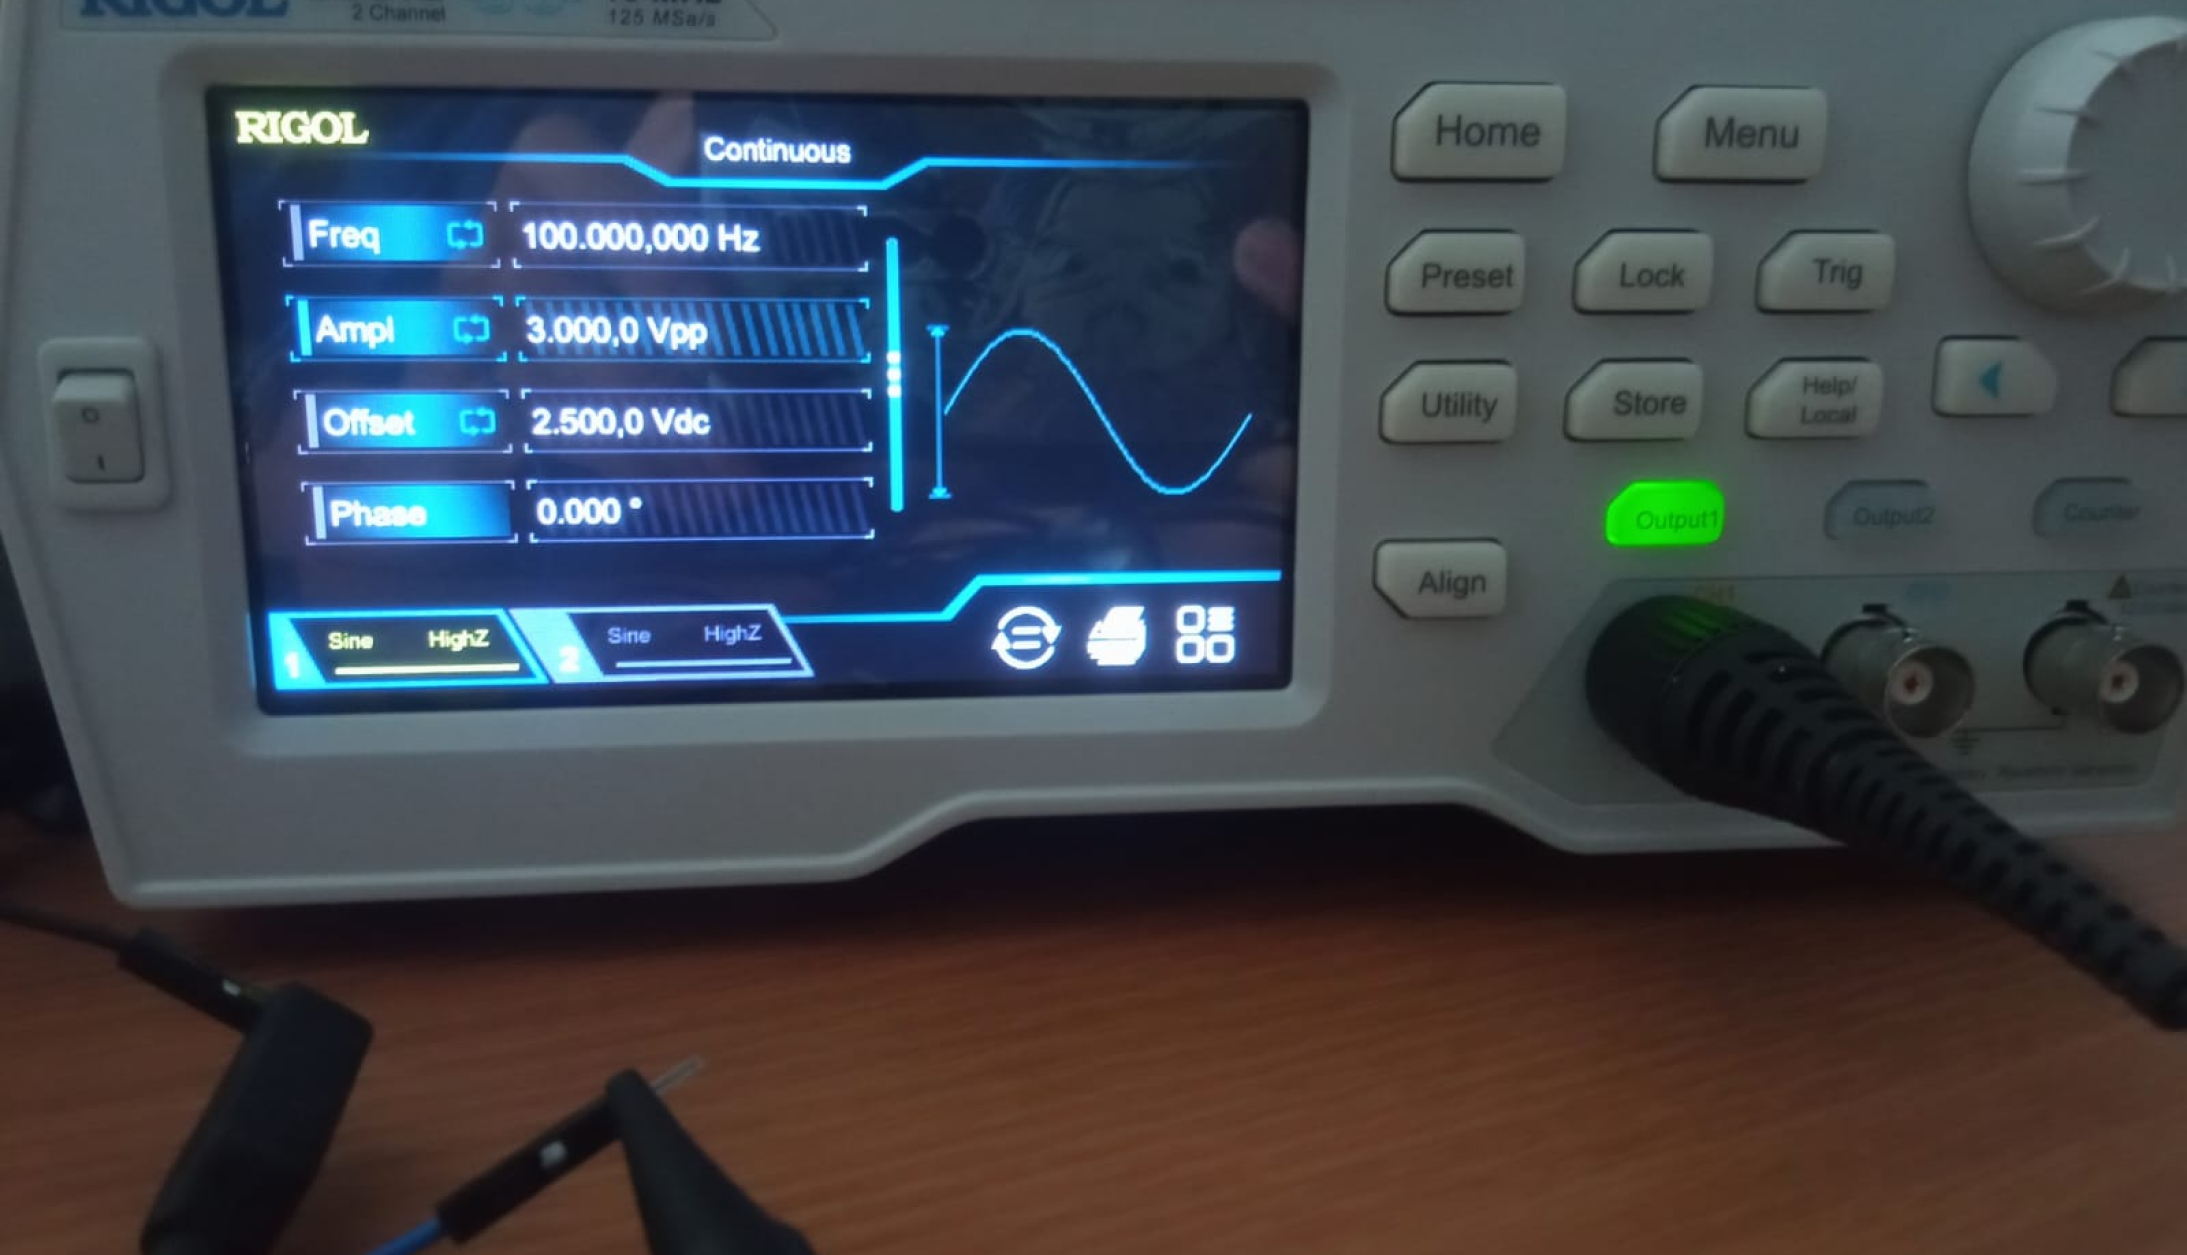
\includegraphics[width=0.8\linewidth]{P4/img/per1/step 7.png}
			\caption{Step 7}
			\label{fig:Step 7(Step 7)}
		\end{figure}
	\end{enumerate}

	\textbf{Konfigurasi Arduino}
	\begin{enumerate}
		\item Hubungkan kabel jumper ke salah satu pin Analog Arduino, kemudian hubungan ke probe.
		\\pengait (positif) Function generator.
		\begin{figure}[H]
			\centering
			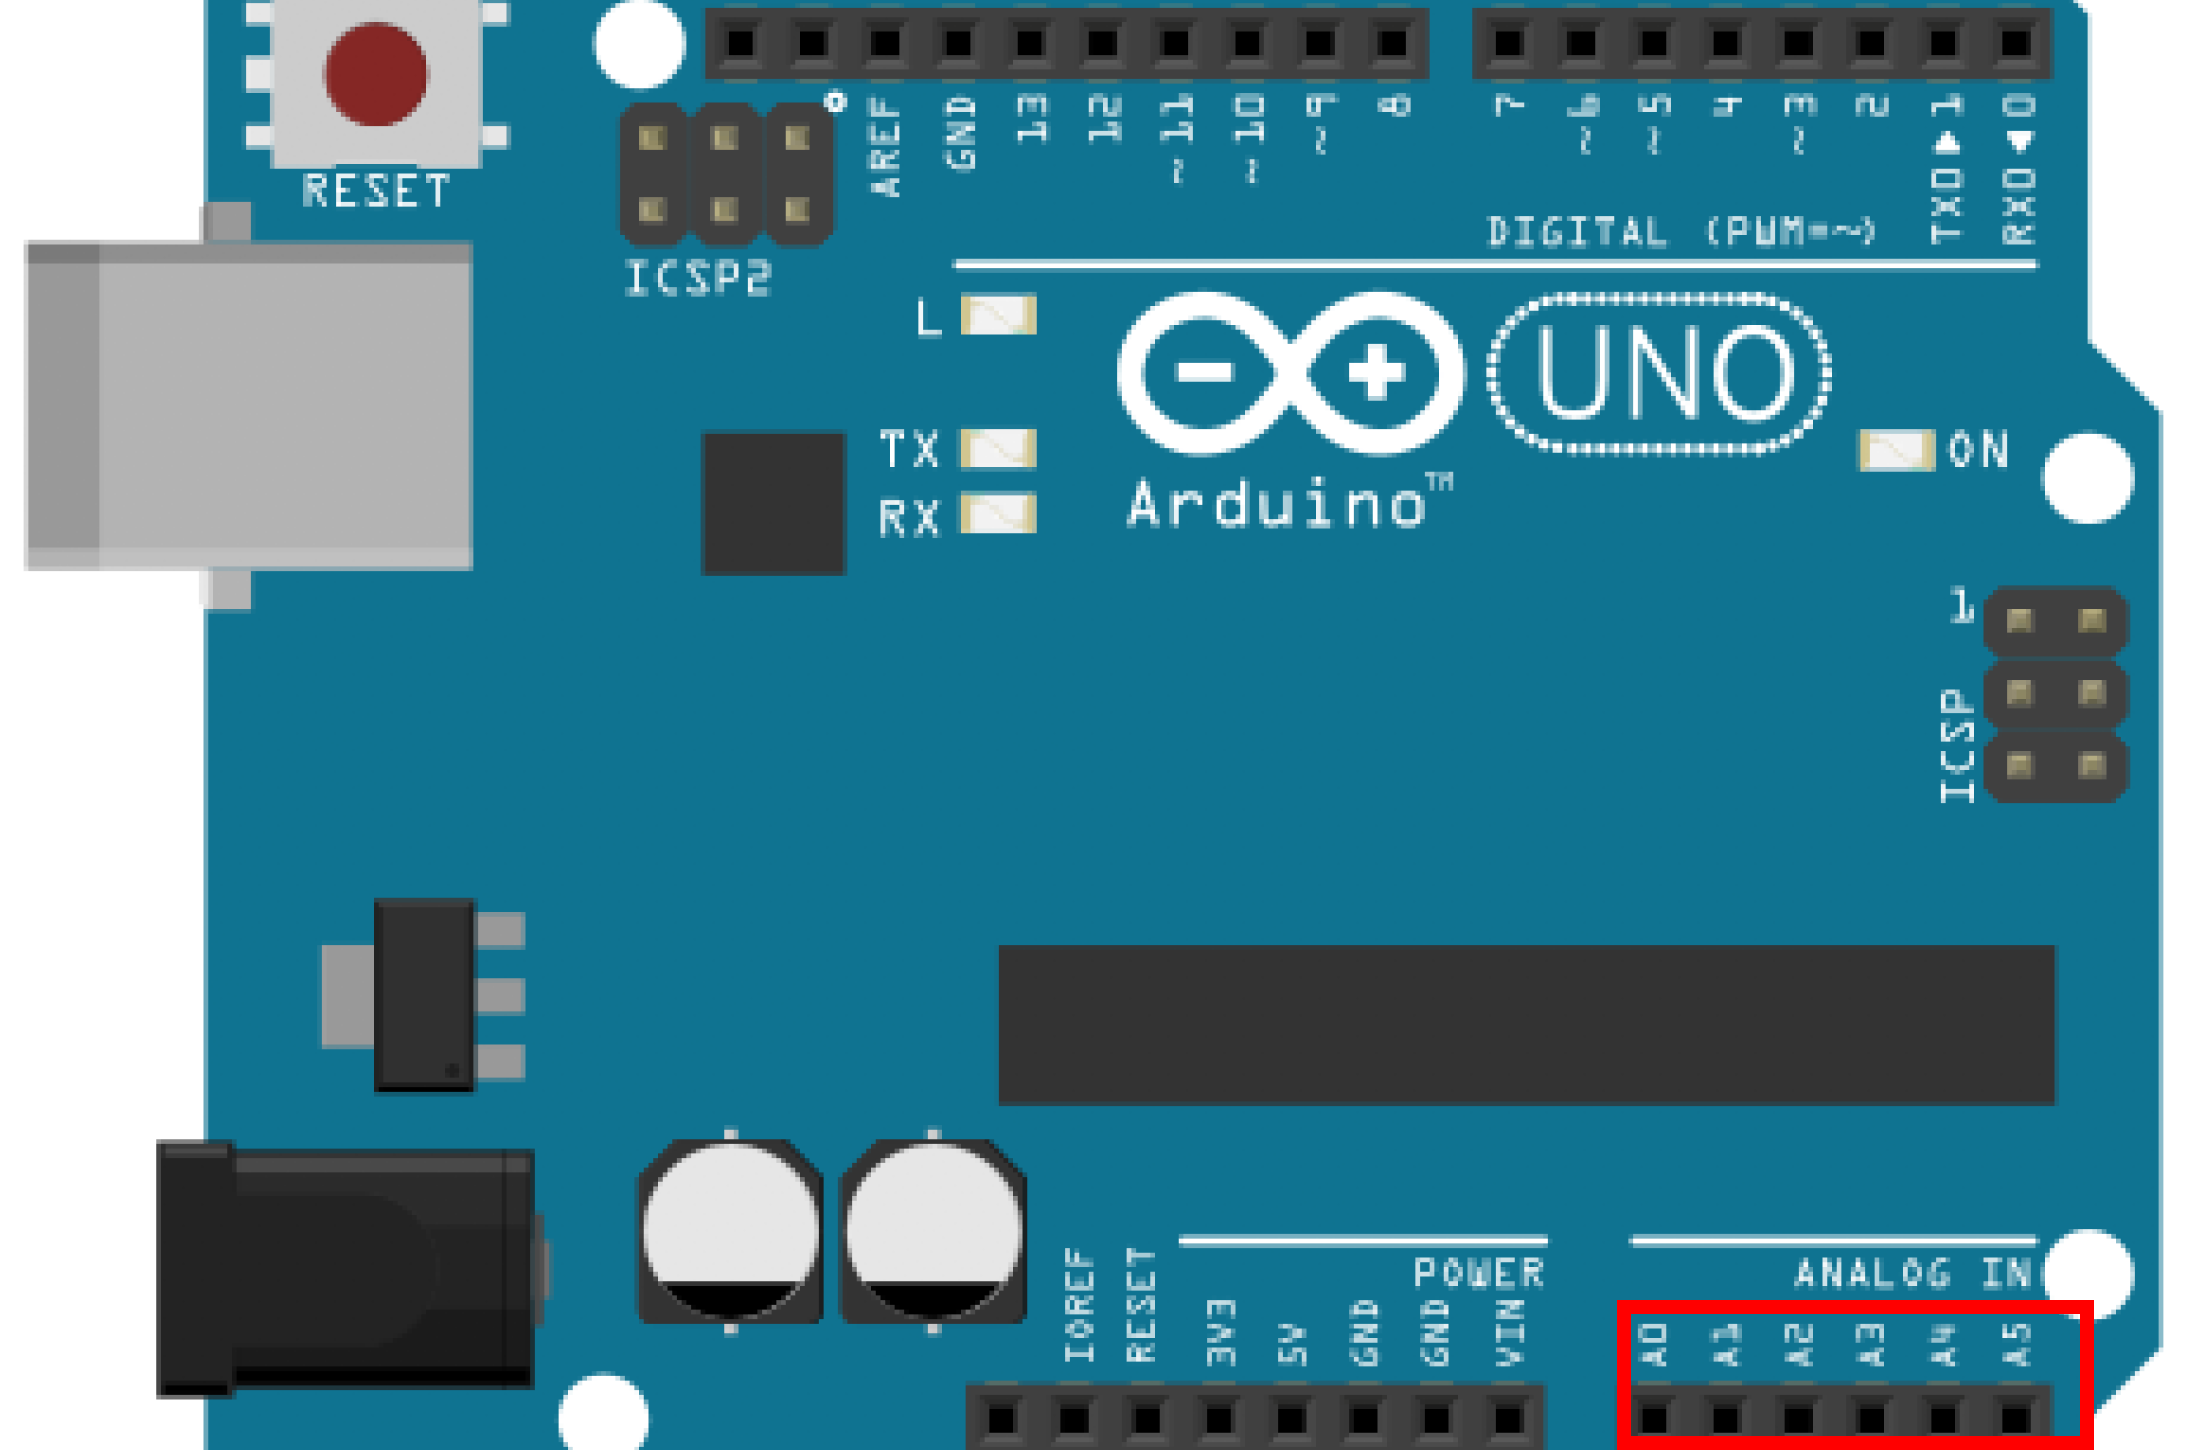
\includegraphics[width=0.8\linewidth]{P4/img/per1/step 8.png}
			\caption{Step 8}
			\label{fig:Step 8(Step 8)}
		\end{figure}

		\item Hubungkan kabel jumper ke salah satu pin GND Arduino, kemudian hubungkan probe.
		\\penjepit buaya (negatif) Function generator.
		\begin{figure}[H]
			\centering
			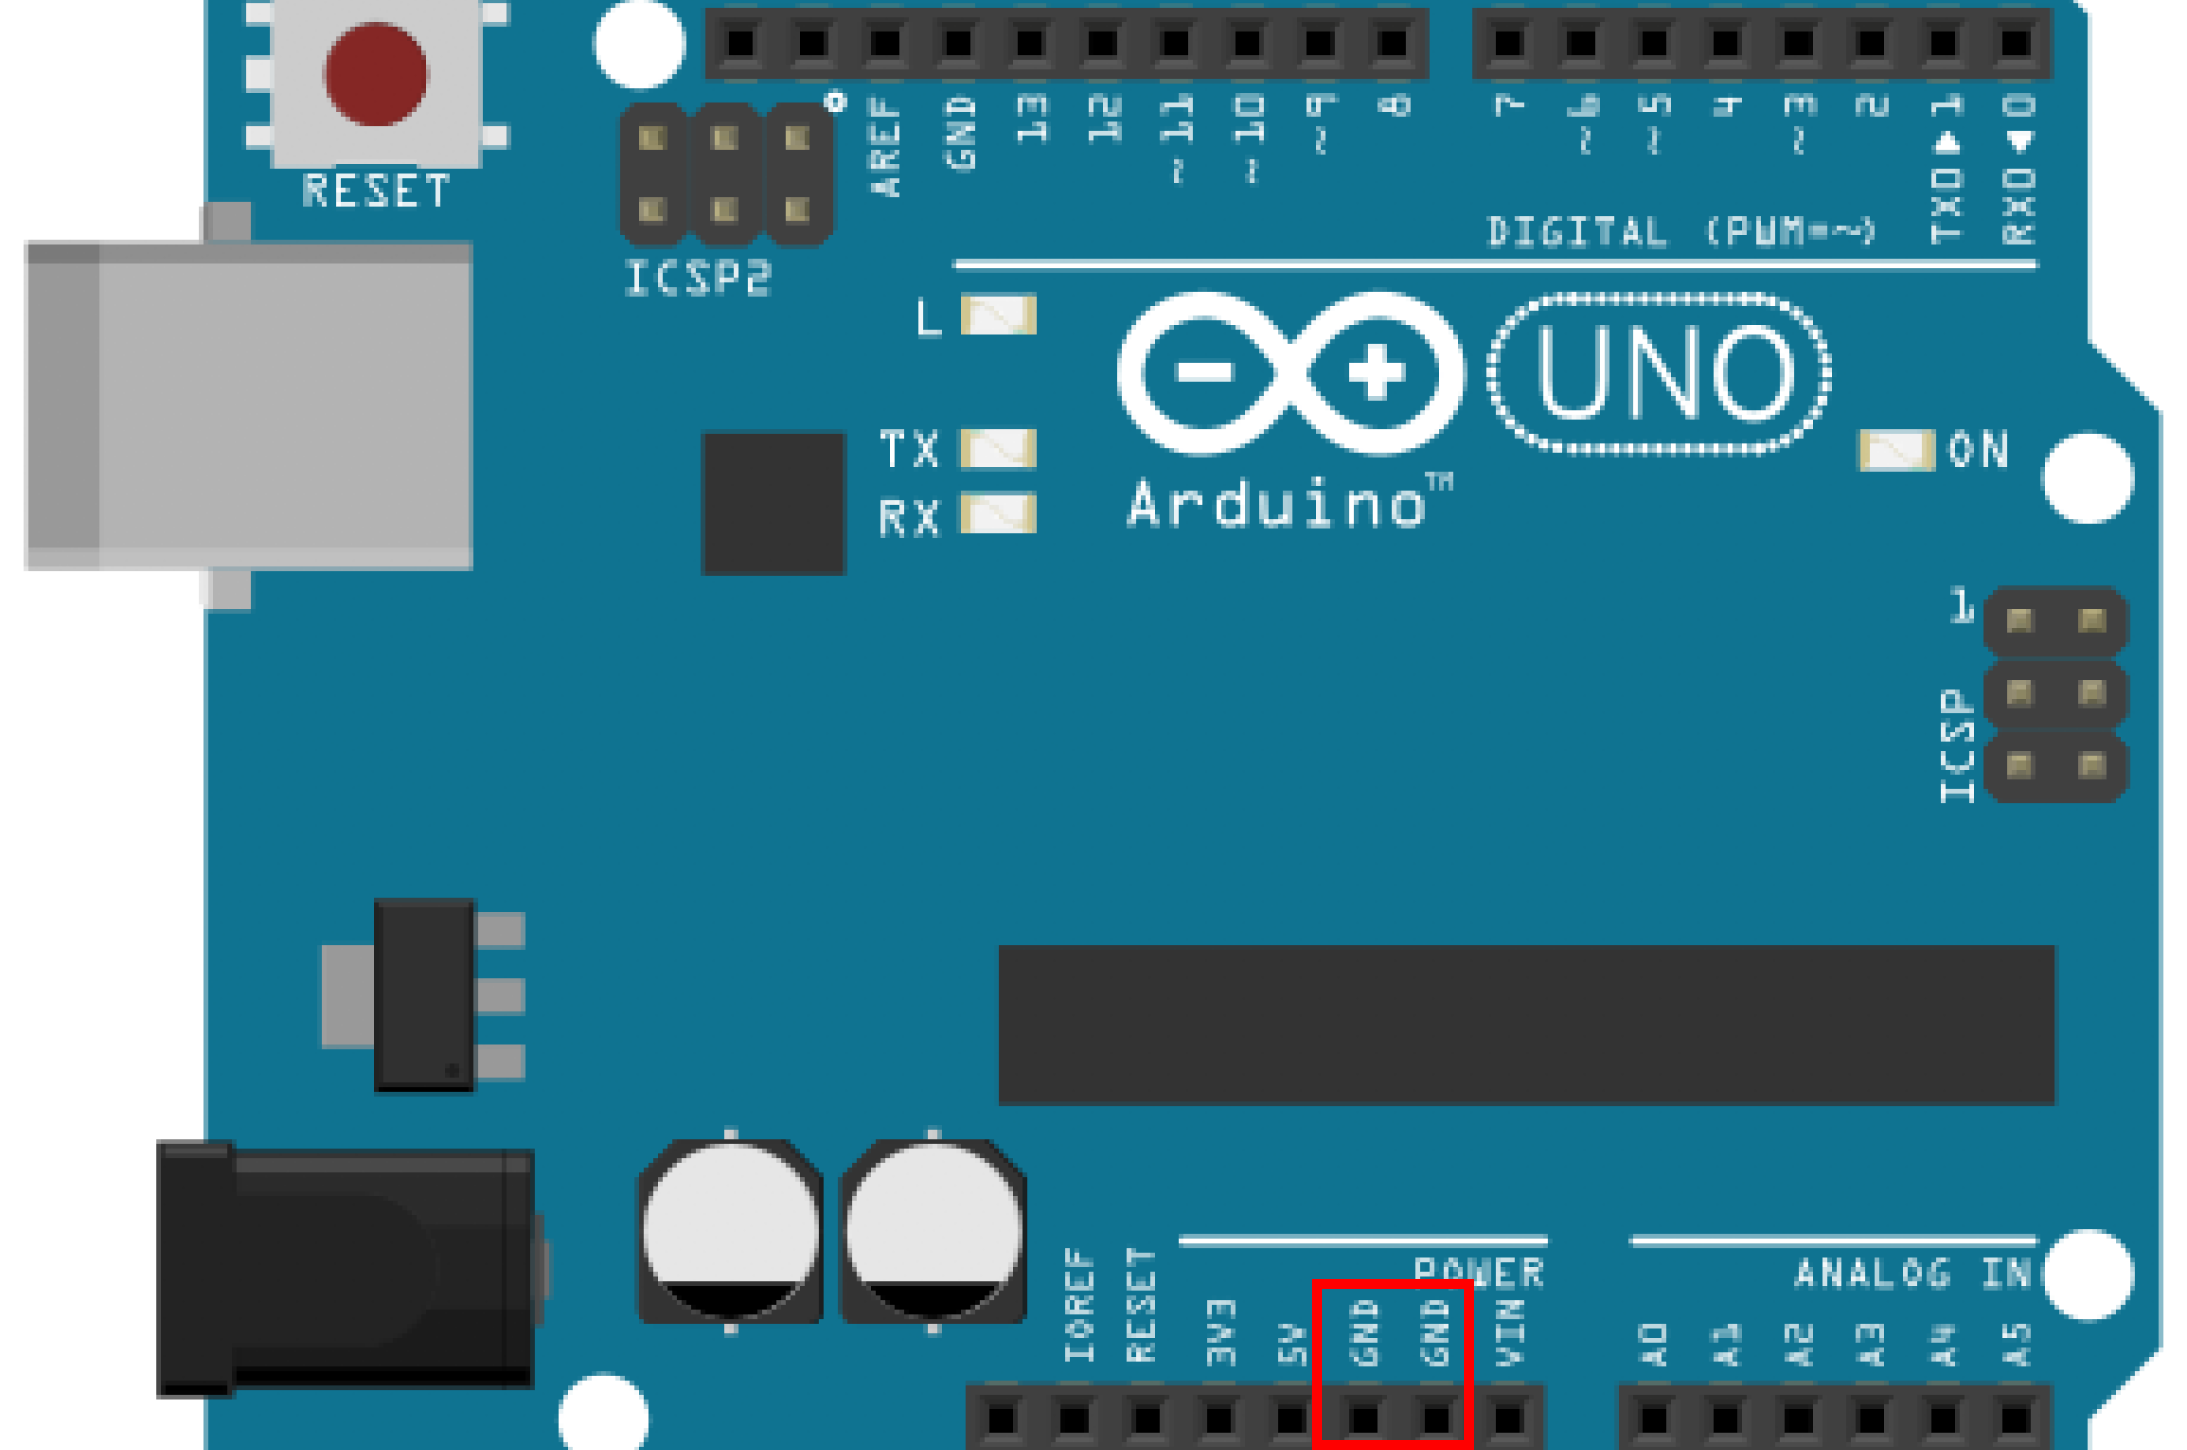
\includegraphics[width=0.8\linewidth]{P4/img/per1/step 9.png}
			\caption{Step 9}
			\label{fig:Step 9(Step 9)}
		\end{figure}

		\item Nyalakan Output 1 pada Function Generator.
		\item Buka Serial plotter di pojok kanan atas pada Arduino IDE.
		\item Buka Serial Monitor di pojok kanan atas pada Arduino IDE.
	\end{enumerate}

\end{center}

%======================PERCOBAAN 2==========================%
\subsection{Percobaan 2}
\begin{center}
	\textbf{Konfigurasi Osiloskop}
	\begin{enumerate}
		\item Hubungkan kabel power ke osiloskop, lalu tekan tombol power untuk menyalakan Osiloskop. 
		\begin{figure}[H]
			\centering
			\includegraphics[width=0.9\linewidth]{P4/img/per2/step 1.png}
			\caption{Step 1}
			\label{fig:Step 1(Step 1)}
		\end{figure}

		\item Hubungkan kabel probe pada channel 1. 
		\begin{figure}[H]
			\centering
			\includegraphics[width=0.8\linewidth]{P4/img/per2/step 2.png}
			\caption{Step 2}
			\label{fig:Step 2(Step 2)}
		\end{figure}

		\item Hubungkan kabel jumper dari salah satu pin Analog Arduino dengan probe pengait (positif) osiloskop dan function generator.
		\item Hubungkan kabel jumper pin GND Arduino dengan probe penjepit buaya (negatif) osiloskop.
		\item Klik AUTO pada Osiloskop.
		\item Bandingkan hasil sinyal yang ditampilkan oleh Serial plotter Arduino dengan Osiloskop.
	\end{enumerate}	
\end{center}

%===========================================================%
\section{Hasil yang didapat}
Memahami perbedaan hasil sinyal digital yang diperoleh oleh Arduino dan Osiloskop.

%===========================================================%
\section{Kesimpulan}
Mengetahui hasil sinyal manakah yang lebih baik dihasilkan dari kedua perangkat \\Arduino dan Osiloskop.

% \section{Pendahuluan}
\subsection{Latar Belakang}
Fourier Transform digunakan untuk mengubah sinyal dari domain waktu (time domain) ke domain frekuensi (frequency domain). 
Dengan menggunakan Fourier Transform, sinyal dapat dianalisis dan dipahami lebih baik dalam hal komponen frekuensinya, amplitudonya, dan fase-nya. 
Fourier Transform sangat penting dalam berbagai aplikasi, seperti pengolahan sinyal audio, pengukuran, dan sistem monitoring.
\\\\
Ada dua jenis utama Fourier Transform: Transformasi Fourier Kontinu (Continuous Fourier Transform) dan Transformasi Fourier Diskrit (Discrete Fourier Transform). 
Transformasi Fourier Kontinu digunakan untuk sinyal kontinu dan didefinisikan dengan integral Fourier. 
Sementara itu, Transformasi Fourier Diskrit digunakan untuk sinyal diskrit dan didefinisikan dengan rumus yang lebih sederhana. 
Dalam prakteknya, Transformasi Fourier Diskrit lebih umum digunakan karena sinyal digital yang digunakan dalam komputer dan sistem lainnya adalah sinyal diskrit.

\subsection{Maksud dan Tujuan}
Memahami dasar-dasar teori Fourier Transform, termasuk perbedaan antara Transformasi Fourier Kontinu dan Diskrit.

\subsection{Hasil yang diharapkan}
Mengetahui perbandingan hasil sinyal Fourier Transform sebelum dan sesudah.

%===========================================================%
\section{Tugas Pendahuluan}
\begin{center}
	\colorbox{cyan!30}{\parbox{0.8\linewidth}{
    \begin{enumerate}
        \item Apa solusi lain ketika IPv4 habis, selain menggunakan IPv6?
        \item Sebutkan tiga keunggulan IPv6 dibandingkan IPv4!
        \item Mengapa panjang awal alamat IPv6 biasanya adalah 128 bit?
    \end{enumerate}}}
\end{center}

%===========================================================%
\section{Alat dan Bahan}
\begin{itemize}[label=$\bullet$, itemsep=-1pt, leftmargin=*]
	\item 1 Perangkat Arduino
	\item 1 Laptop
	\item 1 Osiloskop
	\item 1 Function Generator
	\item Software Arduino IDE
\end{itemize}

%===========================================================%
\section{Jangka Waktu Pelaksanaan}
Pemahaman dan konfigurasi 1 jam.

%===========================================================%
\section{Penjelasan dan Tahapan Konfigurasi}

%======================PERCOBAAN 1==========================%
\subsection{Percobaan 1}
\begin{center}

	\textbf{Memulai Arduino IDE}
	\begin{enumerate}
		\item Hubungkan Arduino Uno dengan laptop.
		\begin{figure}[H]
			\centering
			\includegraphics[width=0.8\linewidth]{P5/img/per1/step 1.png}
			\caption{Step 1}
			\label{fig:Step 1(Step 1)}
		\end{figure}
		\item Buka software Arduino IDE, lalu pilih new sketch.
		\begin{figure}[H]
			\centering
			\includegraphics[width=0.8\linewidth]{P5/img/per1/step 2.png}
			\caption{Step 2}
			\label{fig:Step 2(Step 2)}
		\end{figure}
		\item Buka menu Tools, lalu cek Board dan Port yang terhubung apakah sudah benar
		\\(Port bergantung pada device, jadi bisa berbeda dengan port di Modul).
		\begin{figure}[H]
			\centering
			\includegraphics[width=0.8\linewidth]{P5/img/per1/step 3.png}
			\caption{Step 3}
			\label{fig:Step 3(Step 3)}
		\end{figure}
		\begin{figure}[H]
			\centering
			\includegraphics[width=0.8\linewidth]{P2/img/per1/step 4.png}
			\caption{Step 4}
			\label{fig:Step 4(Step 4)}
		\end{figure}

	
	\textbf{Kode Program Arduino}
		\item Masukkan kode program dibawah ini untuk menjalankan Fourier Transform pada Arduino IDE.
		\begin{figure}[H]
			\centering
			\includegraphics[width=0.8\linewidth]{P5/img/per1/step 5.png}
			\caption{Step 5}
			\label{fig:Step 5(Step 5)}
		\end{figure}
	
		\item Klik verify, apabila berhasil maka klik upload.
	\end{enumerate}
	
	\textbf{Memulai Function Generator}
	\begin{enumerate}
		\item Klik tombol power, untuk menyalakan function generator.
		\begin{figure}[H]
			\centering
			\includegraphics[width=0.8\linewidth]{P5/img/per1/step 6.png}
			\caption{Step 6}
			\label{fig:Step 6(Step 6)}
		\end{figure}

		\item Konfigurasi sinyal input pada Function generator.
		\begin{figure}[H]
			\centering
			\includegraphics[width=0.8\linewidth]{P5/img/per1/step 7.png}
			\caption{Step 7}
			\label{fig:Step 7(Step 7)}
		\end{figure}
	\end{enumerate}

	\textbf{Konfigurasi Arduino}
	\begin{enumerate}
		\item Hubungkan kabel jumper ke salah satu pin Analog Arduino, kemudian hubungan ke probe.
		\\pengait (positif) Function generator.
		\begin{figure}[H]
			\centering
			\includegraphics[width=0.8\linewidth]{P5/img/per1/step 8.png}
			\caption{Step 8}
			\label{fig:Step 8(Step 8)}
		\end{figure}

		\item Hubungkan kabel jumper ke salah satu pin GND Arduino, kemudian hubungkan probe.
		\\penjepit buaya (negatif) Function generator.
		\begin{figure}[H]
			\centering
			\includegraphics[width=0.8\linewidth]{P5/img/per1/step 9.png}
			\caption{Step 9}
			\label{fig:Step 9(Step 9)}
		\end{figure}

		\item Nyalakan Output 1 pada Function Generator.
		\item Buka Serial plotter di pojok kanan atas pada Arduino IDE.
		\item Buka Serial Monitor di pojok kanan atas pada Arduino IDE.
	\end{enumerate}

\end{center}

%======================PERCOBAAN 2==========================%
\subsection{Percobaan 2}
\begin{center}
	\textbf{Konfigurasi Osiloskop}
	\begin{enumerate}
		\item Hubungkan kabel power ke osiloskop, lalu tekan tombol power untuk menyalakan Osiloskop. 
		\begin{figure}[H]
			\centering
			\includegraphics[width=0.9\linewidth]{P5/img/per2/step 1.png}
			\caption{Step 1}
			\label{fig:Step 1(Step 1)}
		\end{figure}

		\item Hubungkan kabel probe pada channel 1. 
		\begin{figure}[H]
			\centering
			\includegraphics[width=0.8\linewidth]{P5/img/per2/step 2.png}
			\caption{Step 2}
			\label{fig:Step 2(Step 2)}
		\end{figure}

		\item Hubungkan kabel jumper dari salah satu pin Analog Arduino dengan probe pengait (positif) osiloskop dan function generator.
		\item Hubungkan kabel jumper pin GND Arduino dengan probe penjepit buaya (negatif) osiloskop.
		\item Klik AUTO pada Osiloskop.
		\item Bandingkan hasil sinyal yang ditampilkan oleh Serial plotter Arduino dengan Osiloskop.
	\end{enumerate}	
\end{center}

%===========================================================%
\section{Hasil yang didapat}
Memahami perbedaan hasil sinyal digital yang diperoleh oleh Arduino dan Osiloskop.

%===========================================================%
\section{Kesimpulan}
Mengetahui hasil sinyal manakah yang lebih baik dihasilkan dari kedua perangkat \\Arduino dan Osiloskop.


\renewcommand\refname{Daftar Pustaka} % Menghilangkan kata "Daftar Pustaka"
\renewcommand{\bibname}{} % Menghilangkan kata "Bibliography"

\printbibliography
\end{document}
